% STANDALONE_COB_BRINGUP_PLAN.tex
% Bring-up plan for a standalone chip-on-board test board, nanoSoC Ethernet
% chiplet rc4-20260829. Build: xelatex (twice). Needs figures/padmap.pdf,
% figures/appC_rows.tex and figures/cob_feasibility.tex, which
% figures/gen_figs.py regenerates from the repository's as-built pad CSV
% (ASIC/submissions/padring_as_built_rzG_20260823/...pads_only.csv).
% Fonts: Lato and DejaVu Sans Mono if installed, else TeX Gyre Heros / Latin
% Modern Mono (both ship with TeX Live).
\documentclass[10pt,a4paper]{article}

\usepackage[a4paper,left=2cm,right=2cm,top=2.3cm,bottom=2.2cm,headheight=14pt,headsep=0.5cm]{geometry}
\usepackage{fontspec}
\IfFontExistsTF{Lato}{\setmainfont{Lato}[Ligatures=NoCommon]}{\setmainfont{TeX Gyre Heros}}
\IfFontExistsTF{DejaVu Sans Mono}{\setmonofont[Scale=0.84]{DejaVu Sans Mono}}{\setmonofont{Latin Modern Mono}}
\usepackage[table]{xcolor}
\usepackage{graphicx}
\usepackage{booktabs}
\usepackage{array}
\usepackage{tabularx}
\usepackage{longtable}
\usepackage{multirow}
\usepackage{enumitem}
\usepackage{titlesec}
\usepackage{fancyhdr}
\usepackage{lastpage}
\usepackage[font=small,labelfont=bf,labelsep=period,skip=4pt]{caption}
\usepackage{float}
\usepackage{needspace}
\usepackage{tikz}
\usetikzlibrary{positioning,arrows.meta,calc,shapes.geometric,fit,backgrounds}
\usepackage[most]{tcolorbox}
\usepackage{url}
\usepackage[hidelinks]{hyperref}
\def\UrlBreaks{\do\/\do\-\do\.\do\_\do\=\do\?\do\&}
\def\UrlFont{\small\ttfamily}

% ---------------------------------------------------------------- colours
\definecolor{accent}{HTML}{1F3A5F}
\definecolor{accent2}{HTML}{2E6DA4}
\definecolor{srcgray}{HTML}{5A6570}
\definecolor{headgray}{HTML}{E3E8EF}
\definecolor{rowgray}{HTML}{F5F7FA}
\definecolor{warn}{HTML}{B03A2E}
\definecolor{ok}{HTML}{2E7D32}
\definecolor{amber}{HTML}{A66300}
\definecolor{gPower}{HTML}{8C8C8C}
\definecolor{gClk}{HTML}{D55E00}
\definecolor{gDbg}{HTML}{0072B2}
\definecolor{gQspi}{HTML}{009E73}
\definecolor{gRmii}{HTML}{E69F00}
\definecolor{gD2d}{HTML}{CC79A7}

% ---------------------------------------------------------------- macros
\DeclareUrlCommand\srcraw{\def\UrlFont{\scriptsize\ttfamily}%
  \def\UrlBreaks{\do\/\do\_\do\-\do\.\do\:\do\,}}
\newcommand\src{\leavevmode\begingroup\color{srcgray}\srcaux}
\newcommand\srcaux[1]{\srcraw{#1}\endgroup}
\DeclareUrlCommand\sig{\def\UrlFont{\ttfamily}\def\UrlBreaks{\do\_\do\/\do\-\do\.\do\,}}
\newcommand\nohyph{\hyphenpenalty=10000 \exhyphenpenalty=10000 }
\newcommand\cmd[1]{\texttt{\detokenize{#1}}}
\newcommand\EX{\textcolor{ok}{\textbf{exists}}}
\newcommand\PA{\textcolor{amber}{\textbf{partial}}}
\newcommand\NW{\textcolor{warn}{\textbf{new}}}
\newcommand\PR{\textcolor{srcgray}{\textbf{proc.}}}
\newcommand\NF{\textcolor{warn}{\textbf{NOT FOUND}}}
\newcommand\hd[1]{\textbf{#1}}
\newcolumntype{L}{>{\raggedright\arraybackslash}X}
\newcolumntype{P}[1]{>{\raggedright\arraybackslash}p{#1}}
\newcolumntype{C}[1]{>{\centering\arraybackslash}p{#1}}

\newtcolorbox{gatebox}{enhanced,colback=accent!5,colframe=accent,boxrule=0pt,
  leftrule=2.5pt,arc=0pt,outer arc=0pt,left=6pt,right=6pt,top=3pt,bottom=3pt,
  before skip=6pt,after skip=8pt,fontupper=\small}
\newtcolorbox{warnbox}{enhanced,colback=warn!5,colframe=warn,boxrule=0pt,
  leftrule=2.5pt,arc=0pt,outer arc=0pt,left=6pt,right=6pt,top=3pt,bottom=3pt,
  before skip=6pt,after skip=8pt,fontupper=\small}
\newtcolorbox{notebox}{enhanced,colback=rowgray,colframe=srcgray,boxrule=0pt,
  leftrule=2.5pt,arc=0pt,outer arc=0pt,left=6pt,right=6pt,top=3pt,bottom=3pt,
  before skip=6pt,after skip=8pt,fontupper=\small}

% phase tables
\newcommand\phasehead{\toprule
  \rowcolor{headgray}[0pt][0pt]\hd{\#} & \hd{Test} & \hd{Pass criterion} & \hd{Path} & \hd{Tool / reference} & \hd{Status}\\
  \midrule}
\newcommand\phasebegin{\par\noindent\begingroup\footnotesize\setlength{\tabcolsep}{4pt}\renewcommand{\arraystretch}{1.22}}
\newcommand\phaseend{\endgroup\par\medskip}

\setlength{\parindent}{0pt}
\setlength{\parskip}{4pt}
\setlist{nosep,leftmargin=1.4em,topsep=2pt}
\renewcommand{\arraystretch}{1.18}
\setlength{\LTpre}{4pt}\setlength{\LTpost}{6pt}

% ---------------------------------------------------------------- headings
\titleformat{\section}{\Large\bfseries\color{accent}}{\thesection}{0.7em}{}
\titleformat{\subsection}{\large\bfseries\color{accent}}{\thesubsection}{0.6em}{}
\titleformat{\subsubsection}{\normalsize\bfseries\color{accent2}}{\thesubsubsection}{0.5em}{}
\titlespacing*{\section}{0pt}{14pt}{6pt}
\titlespacing*{\subsection}{0pt}{10pt}{4pt}
\titlespacing*{\subsubsection}{0pt}{8pt}{3pt}

\pagestyle{fancy}
\fancyhf{}
\fancyhead[L]{\small\color{srcgray}Standalone COB test board: bring-up plan}
\fancyhead[R]{\small\color{srcgray}rc4-20260829 \textperiodcentered{} Draft for review \textperiodcentered{} 2026-09-30}
\fancyfoot[C]{\small\color{srcgray}Page \thepage{} of \pageref{LastPage}}
\renewcommand{\headrulewidth}{0.4pt}
\renewcommand{\headrule}{\hbox to\headwidth{\color{headgray}\leaders\hrule height \headrulewidth\hfill}}

\hypersetup{pdftitle={Standalone COB test board: bring-up plan (rc4-20260829)},
  pdfauthor={SoC Labs nanoSoC Ethernet chiplet team},
  pdfsubject={Bring-up plan, draft for review, 2026-09-30}}

\begin{document}

% =====================================================================
% TITLE PAGE
% =====================================================================
\begin{titlepage}
\thispagestyle{empty}
\vspace*{1.6cm}
{\color{accent}\rule{\linewidth}{1.6pt}}\par
\vspace{0.7cm}
{\fontsize{26}{31}\selectfont\bfseries\color{accent} Standalone Chip-on-Board Test Board\par}
\vspace{0.25cm}
{\fontsize{19}{23}\selectfont Bring-up Plan\par}
\vspace{0.3cm}
{\large\color{accent2} Motherboard + interchangeable card: bonded-die card or K26 FPGA card\par}
\vspace{0.5cm}
{\large nanoSoC Ethernet chiplet \textperiodcentered{} TSMC 65 nm LP \textperiodcentered{} submitted candidate \textbf{rc4-20260829}\par}
\vspace{0.6cm}
{\color{accent}\rule{\linewidth}{0.6pt}}\par
\vspace{0.9cm}
{\renewcommand{\arraystretch}{1.45}
\begin{tabularx}{\linewidth}{@{}P{3.6cm}L@{}}
\hd{Design} & nanoSoC Ethernet chiplet, candidate \textbf{rc4-20260829} (submitted to Europractice / imec on 1 September 2026) \\
\hd{Date} & 2026-09-30 \\
\hd{Status} & \textbf{Draft for review} \\
\hd{Audience} & The lab's bring-up engineers and the PCB designer. Hardware- and firmware-literate; familiar with the project, not assumed to know every erratum. \\
\hd{Scope} & A bring-up \textbf{motherboard} with one card slot, and \textbf{interchangeable cards} for that slot: the \textbf{die card} (one bare die wire-bonded, chip-on-board, to a small card) and the \textbf{K26 FPGA card} (a Kria K26I SOM running the chiplet emulator), used to bring the motherboard up first; optionally a packaged-die card. The die is brought up without the compute chiplet. The TideLink die-to-die interconnect is \textbf{out of scope}: the die card only parks its pins safely. \\
\hd{Repository state read} & \sig{SoC-Labs/NanoSoC-Ethernet-Chiplet} at \sig{914c9e4} (branch \sig{feat/padring-boundary-scan}); \sig{nanosoc-multicore-system} at \sig{2adcd34}, whose boot code, include files and RTL are identical to the rc4 pin \sig{f60449b}. \\
\end{tabularx}}
\vfill
\begin{notebox}
\textbf{How to read this document.} Section~\ref{sec:summary} is the one-page summary. Section~\ref{sec:board} is the PCB designer's section; Section~\ref{sec:slot} defines the slot between motherboard and card. Sections~\ref{sec:prep} and~\ref{sec:phases} are the bench procedure: Phase M (motherboard with the K26 FPGA card), then phases P0--P15 on the die card, each ending in a gate that must pass before the next phase starts.\\[3pt]
Source references are printed small and grey, e.g.\ \src{REG:170-196}. They are \emph{path:line} references into the repository; the short aliases (REG, PROC, BSC, \dots) are expanded in Appendix~\ref{app:refs}.\\[3pt]
\textbf{NOT FOUND} means the fact was searched for in the repository and is not recorded there. Every NOT FOUND item is carried as an open question in Section~\ref{sec:risks}.\\[3pt]
\textbf{Vendor data.} This file lives in a public repository. TSMC IO-library parameters (pull resistances, input thresholds, drive currents, EM limits) are therefore not reproduced; read them from the site-licensed IO databook (\src{ASIC/tech_wrappers/tsmc65/README.md:21-24}).
\end{notebox}
\end{titlepage}

\setcounter{page}{2}
\tableofcontents
\newpage

% =====================================================================
\section{Summary}\label{sec:summary}
% =====================================================================
\textbf{What the board proves.} The board is a \textbf{motherboard with one card slot} that takes \textbf{interchangeable cards}: the \textbf{die card} carrying one wire-bonded rc4 die, or the \textbf{K26 FPGA card} running the chiplet emulator. The die goes from first power to Ethernet traffic with no compute chiplet attached. The phases in Section~\ref{sec:phases} establish, in order:

{\small
\renewcommand{\arraystretch}{1.2}
\begin{tabularx}{\textwidth}{@{}P{1.9cm}L@{}}
\toprule
\rowcolor{headgray}[0pt][0pt]\hd{Phases} & \hd{What passing proves} \\
\midrule
M & The motherboard works before any die is at risk: rails, clocks, flash programming path, PHY link, HOSTIO header and host-MCU scripting, proven with the K26 FPGA card. \\
P0--P1 & The die card is bonded without shorts or opens. Supplies, clock and reset behave. Current draw is plausible. \\
P2 & The pad ring and the boundary-scan TAP work, independently of the core. \\
P2b & \textbf{New (B-1).} With the DNP loopback footprints fitted: TL pad continuity, then one die trains the shipped D2D configuration against itself. \\
P3--P7 & The HOSTIO4 host link works. Both boot ROMs ran. Clock, PHC, registers and all five RAMs respond. \\
P8 & Whether SWD attaches on a die. SWD has answered on FPGA but never on a die: DPIDR \texttt{0x6BA02477} on the HAPS-SX eth-chiplet build (2026-09-09) and on the KR260 eth image (2026-10-02), and the silicon eth ROM read through AP0 on the HAPS-SX BLD-4b mirror (2026-09-30). \\
P9--P11 & The QSPI flash path boots both CPUs. \textbf{This is the critical path.} \\
P12--P14 & On-chip peripherals; Ethernet MAC + RMII PHY to a host PC (ping, UDP echo, throughput); PHC and PTP. \\
P15 & Voltage and frequency shmoo: 50 to 100\,MHz, VDD 1.00 to 1.20\,V. \\
\bottomrule
\end{tabularx}}

Not testable on a standalone board: a two-die TideLink link, and UART, PPS and GPIO (none of them has a pad). With the B-1 loopback footprints fitted, one die can train the shipped D2D configuration against itself (P2b).

\textbf{The critical path is flash provisioning.}
\begin{itemize}
\item CPU0 (the network core) is the only core that reaches the Ethernet MAC. CPU1 and the HOSTIO master do not decode \texttt{0x40000000} \src{REG:210-217,259}.
\item CPU0 always starts in its mask ROM. The ROM copies CPU0's image from QSPI flash into IMEM and halts if the CRC fails \src{ROM0:209-250}.
\item HOSTIO and CPU1 cannot redirect CPU0. The eth REMAP register at \texttt{0x50002000} is decoded only by the debug access port (DAP) \src{REG:259}.
\item The DAP's only port is SWD. The register says SWD never returned a DPIDR \src{REG:215-216}; that is out of date. SWD has answered on FPGA but never on a die: DPIDR \texttt{0x6BA02477} on the HAPS-SX eth-chiplet build (2026-09-09) and on the KR260 eth image (2026-10-02), and the silicon eth ROM read through AP0 on the HAPS-SX BLD-4b mirror (2026-09-30). On a die it is still unproven, so flash stays the plan of record.
\end{itemize}
So the board must let the flash be programmed off-board, through a mux and a programmer header, or be replaced by an SPI-NOR emulator. Every phase from P11 onwards depends on this.

\textbf{Five things that must exist before first power-on.}
\begin{enumerate}
\item \textbf{A motherboard that passed Phase M with the K26 FPGA card,} carrying: a CLK oscillator with an output-enable (OE) pin, run at 50\,MHz; a reset supervisor on NRST; an adjustable, current-monitored core rail; the IOACK pull-up; the QSPI\_IO1 pull-down; CARD\_ID and CARD\_READY gating; scope points. \textbf{A die card} with TEST and SE held low and TL\_RX/TL\_CLK\_RX tied down.
\item \textbf{A route to CPU0 code that does not need SWD.} A QSPI flash behind a mux with an off-board programmer header, plus an emulator header. The part must accept the ROM's commands \texttt{0x0B}, \texttt{0x06}, \texttt{0x02}, \texttt{0x05} and \texttt{0x98}.
\item \textbf{Pre-built, checked flash images.} Start with a TABLE0-only image, packed with \sig{flash_pack.py} and passed by \sig{check_flash.py}.
\item \textbf{The HOSTIO host stack, verified on the bench before the die is powered.} This means the status-nibble fix, the resync watchdog, capture to file, and \cmd{--target asic_tsmc65}.
\item \textbf{A first-power script and record sheet.} They cover the diode checks, current limits, NRST release with CLK stopped, and an address blocklist enforced in the tools.
\end{enumerate}

\begin{gatebox}
\textbf{First action:} email Zepler Cleanrooms (\sig{zepler.cleanrooms@soton.ac.uk}) and settle the bonder, wire type (Au ball or Al wedge), stage size and card-thickness limit, finger size and pitch, and fiducials. That choice fixes the \emph{die card's} finish (ENIG + gold edge fingers for Al; ENEPIG for Au) and its chip-on-board footprint, so it gates the card layout. The motherboard can be laid out in parallel.\\
\textbf{At the same time,} ask imec for the sawn die size, die thickness and backside connection, a PadShorts/ERC run on the rc4 GDS, and the POC and power-sequencing note (Section~\ref{sec:risks}).
\end{gatebox}

\newpage
% =====================================================================
\section{Die and interface}\label{sec:die}
% =====================================================================
\subsection{Die facts}
{\small
\begin{longtable}{@{}P{3.4cm}P{9.1cm}P{3.6cm}@{}}
\toprule
\rowcolor{headgray}[0pt][0pt]\hd{Item} & \hd{Value} & \hd{Source}\\
\midrule
\endfirsthead
\toprule
\rowcolor{headgray}[0pt][0pt]\hd{Item} & \hd{Value} & \hd{Source}\\
\midrule
\endhead
Candidate & rc4-20260829. Submitted 1 Sep 2026. GDS md5 \texttt{6b0833c4\dots} & \src{REG:6-9} \\
Process, IO library & TSMC 65\,nm LP. IO library \sig{tphn65lpgv2od3_sl}: staggered, 2.5\,V devices, 3.3\,V-capable & \src{ASIC/genus-innovus/scripts/nanosoc_eth_chiplet_pads.mmmc:26} \\
Die size & Design frame \textbf{1600 $\times$ 2000\,\textmu m}. With the imec seal ring \textbf{1640 $\times$ 2040\,\textmu m}; add 20\,\textmu m to every design-frame coordinate. IO box 135--1465 $\times$ 135--1865; core 205--1395 $\times$ 205--1795 & FP:12-14; \src{docs/plans/TAPEOUT_PUNCHLIST_2026-08-24.md:24-28} \\
Sawn size, scribe, thickness, backside & \NF. Seal-ring width was asked of the broker and never answered & \src{docs/tapeout/55-imec-preliminary-gds-submission-checklist.md:488} \\
Pads & \textbf{82 IO cells, 82 bond pads} (48 signal + 34 supply) and 4 corner cells. Every IO cell has a bond pad; bond all 82 & \src{PNR:1316477-1316558}; CSV \\
Bond-pad rows & Staggered, two rows. Outer row \sig{PAD70GU_SL} (42 pads), inner row \sig{PAD70NU_SL} (40 pads) & CSV \\
Pitch & Alternating 80\,\textmu m (160\,\textmu m same-row) on the top, right and bottom edges. Alternating 67\,\textmu m (134\,\textmu m same-row) on the left (D2D) edge & CSV; \src{docs/tapeout/60-waiver-document-rc1v3r4.md:158-165} \\
Bond opening & 58\,\textmu m along the edge $\times$ 66\,\textmu m deep. Opening centre 36.8\,\textmu m (outer) or 138.8\,\textmu m (inner) from the design-frame edge; the rows are 102\,\textmu m apart. Measured from imec's rc4 BND marker GDS & \src{REG:500-502}; research report 01 \\
Supplies & One power domain; no analogue or PLL rail. VDD $\times$6 and VSS $\times$4 on the top and bottom edges only. VDDIO $\times$12 (one of them \sig{PVDD2POC_G}) and VSSIO $\times$12, three of each per side & \src{PADS:240-270}; \src{PNR:1321714-1321743} \\
VDDIO level & \textbf{3.3\,V, decided (B-2).} rc4 STA and the UPF used 3.3\,V IO; two docs say 2.5\,V, but those views were never timed & \src{UPF:110-112}; \src{docs/tapeout/10-tapeout-submission.md:163} \\
Clocks & \sig{CLK}: no PLL, no divider, \cmd{SYS_HCLK = SYS_FCLK}; also aliased to \sig{rtc_clk} and \sig{user_ref_clk}. \sig{RMII_REF_CLK}: 50\,MHz input. \sig{SWDCK} constrained to 25\,MHz & \src{PRMU:87-93}; \src{SDC:12-14} \\
Reset & NRST is the only reset pad. There is no on-die POR cell & \src{PRMU:133-157} \\
Cores & Two Cortex-M0+. CPU1 (chip core) runs from power-on and owns the fabric clock and reset. CPU0 (network core) is held until CPU1 sets \texttt{0x29000000} bit 2 & \src{PLAN:332-346} \\
Host ports & SWD (2 pins) and HOSTIO4/ADP (7 pins) only. No UART, GPIO, PPS or CPU-visible I\textsuperscript{2}C pad & \src{PROC:131-134}; \src{CB:137-140} \\
Boundary scan & IDCODE \texttt{0x10001001}, IR length 4, 76-cell boundary register. TAP shares SWD and HOSTIO[0:1] pins; SE is TRST\_n & \src{PTAB}; \src{BSC:77-95} \\
Boot ROMs & \sig{stage0_bootrom_chip_core} (CPU1) and \sig{stage0_bootrom} (CPU0). Both verified bit-exact against the rc4 GDS & \src{REG:535-536} \\
Timing sign-off & 100\,MHz target. Setup +15\,ps at SS/1.08\,V/125\,\textdegree C. Hold checked at FF corners only. Trust about 95\,MHz on slow parts; keep VDD $\le$ 1.2\,V & \src{REG:350-353,445-456} \\
\bottomrule
\end{longtable}\addtocounter{table}{-1}}

\subsection{Pad-ring map}
Figure~\ref{fig:padmap} is drawn from the as-built pad CSV. Each coloured square is a bond opening at its measured position and size. The script that draws it corrects one CSV defect: row 9 (\sig{BuPAD_HOST_IO_6}) says \sig{edge=top}, but the pad is on the \textbf{right} edge; its IO cell and its x coordinate both put it there.

\begin{figure}[p]
\centering
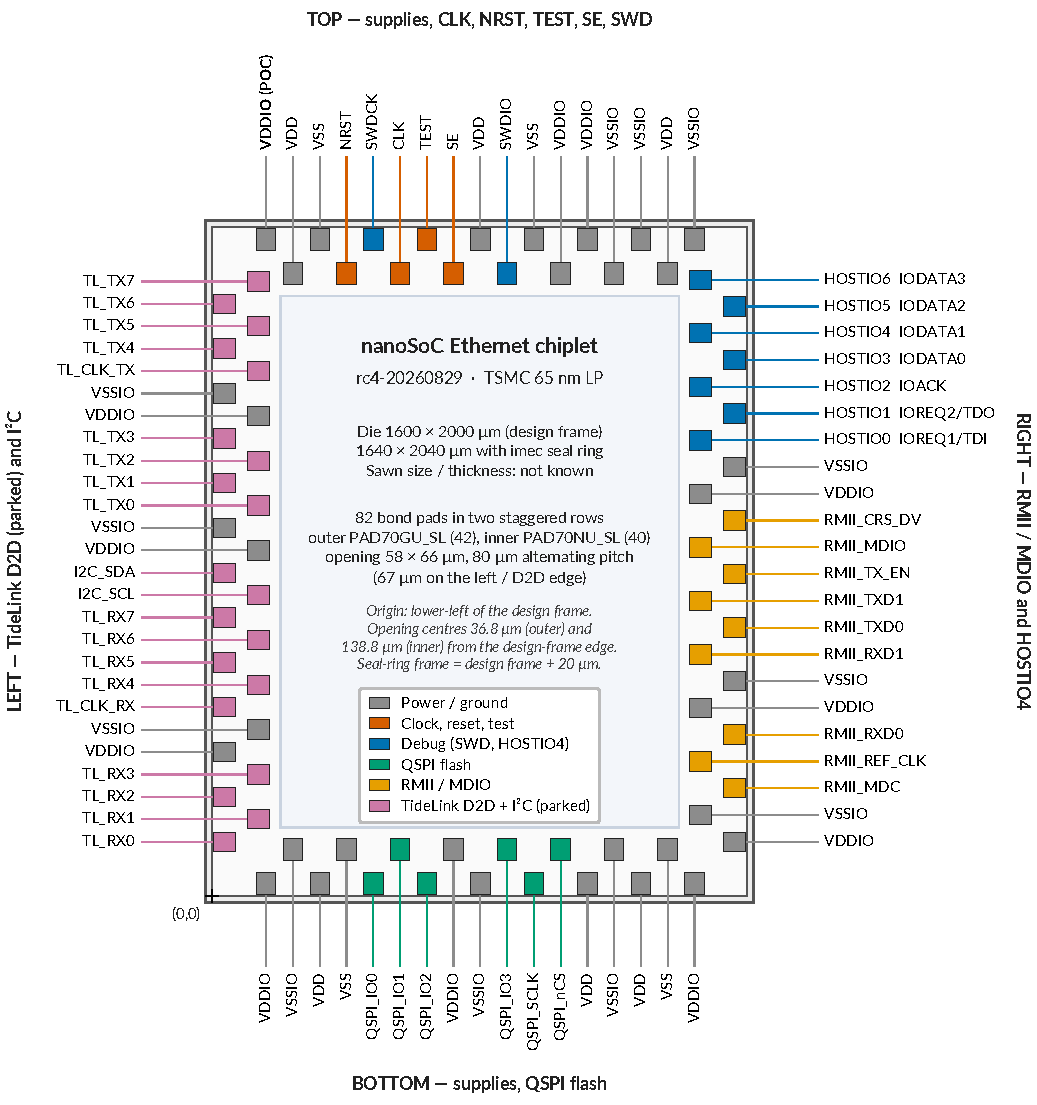
\includegraphics[width=\textwidth]{figures/padmap.pdf}
\caption[Pad-ring map]{Pad-ring map of the rc4 die, design frame, viewed from the top (pad side), origin lower-left. The squares are bond openings drawn to scale (58 $\times$ 66\,\textmu m) in their staggered outer and inner rows. The bold label is the single POC supply pad, \sig{VDDIO_T_0}. Source: \src{CSV}, drawn by \sig{figures/gen_figs.py}.}
\label{fig:padmap}
\end{figure}

\subsection{Pads by function}\label{sec:padtable}
``On-die pull'' is the rc4 netlist state of each pad's pull enable (\sig{REN}, active-low), traced through the buffer chains. It is not just the source default \src{PTAB}; \src{PNR:1321639-1322799}. Where it says \textbf{none}, the board must bias the pin. Section~\ref{sec:partition} says which of these parts sit on the die card and which on the motherboard.

{\footnotesize
\setlength{\tabcolsep}{4pt}
\begin{longtable}{@{}P{2.35cm}P{1.6cm}P{1.9cm}P{1.2cm}P{6.4cm}P{2.1cm}@{}}
\toprule
\rowcolor{headgray}[0pt][0pt]\hd{Pad(s)} & \hd{Direction} & \hd{Cell} & \hd{On-die pull} & \hd{Required board handling} & \hd{Source}\\
\midrule
\endfirsthead
\toprule
\rowcolor{headgray}[0pt][0pt]\hd{Pad(s)} & \hd{Direction} & \hd{Cell} & \hd{On-die pull} & \hd{Required board handling} & \hd{Source}\\
\midrule
\endhead
\multicolumn{6}{@{}l}{\cellcolor{gClk!18}\textbf{Clock, reset, test}}\\
\sig{CLK} & in & \sig{PDDW04DGZ} (non-Schmitt) & \textbf{none} & CMOS oscillator with OE, \textbf{50\,MHz for boot} (B2). Series 22--33\,\textohm{} at the source. A weak pull-down holds the net low while OE disables the oscillator. Max input transition 1.2\,ns. Test point & \src{PADS:551}; \src{SDC:66-67} \\
\sig{NRST} & in, active-low & \sig{PDDW04DGZ} & \textbf{none} & Push-pull supervisor output. Button and host MCU drive the supervisor's manual-reset (MR) input. Must never float. Edge $\le$ 5\,ns. Test point & \src{PADS:567}; \src{SDC:71-72} \\
\sig{TEST} & in & \sig{PDDW04DGZ} & pull-down & Tie low: 0\,\textohm{} or 10\,k\textohm{} to VSS, plus a test point. High bypasses the reset and HOSTIO synchronisers & \src{PADS:559}; \src{PROC:204-220} \\
\sig{SE} & in & \sig{PDDW04DGZ} & pull-down & 10\,k\textohm{} pull-down plus a jumper to VDDIO; also the JTAG header's TRST\_n. \sig{SE}=1 enables the boundary-scan TAP and turns HOSTIO[0:1] into TDI/TDO & \src{PADS:542}; \src{BSC:87-95} \\
\multicolumn{6}{@{}l}{\cellcolor{gDbg!15}\textbf{Debug: SWD (TCK/TMS in boundary scan) and HOSTIO4}}\\
\sig{SWDCK} & in & \sig{PDDW04DGZ} & pull-down & SWD header SWCLK, 22--33\,\textohm{} series. Isolation link to the JTAG header (TCK) & \src{PADS:584} \\
\sig{SWDIO} & bidir & \sig{PDUW08DGZ} & pull-up & SWD header SWDIO, 22--33\,\textohm{} series. Isolation link to the JTAG header (TMS) & \src{PADS:576} \\
\sig{HOSTIO[0]} & bidir: IOREQ1 out; TDI when SE=1 & \sig{PDDW16DGZ} & \textbf{none} & 330\,\textohm{} series; 10\,k\textohm{} idle pull-up; scope test point. Isolation link to the JTAG header & \src{PADS:643-697}; \src{PROC:163-188} \\
\sig{HOSTIO[1]} & bidir: IOREQ2 out; TDO when SE=1 & \sig{PDDW16DGZ} & \textbf{none} & 330\,\textohm{} series; 10\,k\textohm{} idle pull-up. Isolation link to the JTAG header & same \\
\sig{HOSTIO[2]} & bidir: \textbf{IOACK} in, async & \sig{PDDW16DGZ} & \textbf{none} & \textbf{Pull-up mandatory}, about 5\,k\textohm{}, on the die side. Low or floating wedges the HOSTIO FSM in TXC1. 330\,\textohm{} series; scope test point & \src{PROC:221-246} \\
\sig{HOSTIO[3:6]} & bidir: IODATA[0:3] & \sig{PDDW16DGZ} & \textbf{none} & 330\,\textohm{} series; 10\,k\textohm{} idle pull-ups & \src{PROC:221-246} \\
\multicolumn{6}{@{}l}{\cellcolor{gQspi!15}\textbf{QSPI flash}}\\
\sig{QSPI_SCLK} & out, always driven & \sig{PDDW16DGZ} & n/a & 22--33\,\textohm{} series at the die; through the mux to the flash; test point & \src{PADS:593-640} \\
\sig{QSPI_nCS} & out, always driven & \sig{PDDW16DGZ} & n/a & 10\,k\textohm{} pull-up on the flash side, which keeps the flash deselected during ramps and mux switching & same \\
\sig{QSPI_IO0} & bidir & \sig{PDDW16DGZ} & \textbf{none} & Weak pull-up on the die side (the die drives it high at idle in single-SPI mode) & \src{qspi_controller.sv:673-676} \\
\sig{QSPI_IO1} & bidir & \sig{PDDW16DGZ} & \textbf{none} & \textbf{Pull-down, 10\,k\textohm{}, on the die side.} With blank or absent flash the boot then parks in 1.0\,ms, not after a 27.5\,s busy-bit poll at 50\,MHz (rc4-RTL sim, B-6). Test point & \src{REG:242-252}; \src{docs/chip-reference-manual/review/closure/item08-bringup-dryrun.md} \\
\sig{QSPI_IO2/IO3} & bidir & \sig{PDDW16DGZ} & \textbf{none} & Pull-ups on both sides of the mux: they are the flash's WP\# and HOLD\# & \src{PADS:593-640} \\
\multicolumn{6}{@{}l}{\cellcolor{gRmii!18}\textbf{RMII and MDIO}}\\
\sig{RMII_REF_CLK} & \textbf{in} & \sig{PDDW04DGZ} & \textbf{none} & 50\,MHz from an oscillator through a fan-out buffer, length-matched to the PHY. DNP 0\,\textohm{} option to take the PHY's REF\_CLK output instead. Weak pull-down; test point & \src{PADS:700-770}; \src{SDC:13} \\
\sig{RMII_RXD0/1}, \sig{CRS_DV} & in & \sig{PDDW04DGZ} & pull-down & Direct to the PHY, short traces & same \\
\sig{RMII_TXD0/1}, \sig{TX_EN} & out, always driven & \sig{PDDW16DGZ} & n/a & 22--33\,\textohm{} series & same \\
\sig{RMII_MDC} & out, always driven & \sig{PDDW16DGZ} & n/a & 22--33\,\textohm{} series; test point & same \\
\sig{RMII_MDIO} & bidir & \sig{PDDW16DGZ} & \textbf{none} & \textbf{External pull-up, about 1.5\,k\textohm{}.} An inadequate pull-up caused the KR260 MDIO fault. Test point & \src{PROC:881} \\
\multicolumn{6}{@{}l}{\cellcolor{gD2d!18}\textbf{TideLink D2D and I\textsuperscript{2}C sideband (parked; out of test scope)}}\\
\sig{TL_RX[7:0]}, \sig{TL_CLK_RX} & in & \sig{PDDW16DGZ} & \textbf{none} & Bond them, then pull each to VSSIO through 10\,k\textohm{}. Left unbonded they float on the die & \src{PADS:846-917} \\
\sig{TL_TX[7:0]}, \sig{TL_CLK_TX} & out, always driven & \sig{PDDW16DGZ} & n/a & \textbf{Cannot be tri-stated, even in EXTEST. Never tie to a rail.} Bond them (B-1); route to test points and to DNP 0\,\textohm{} TX[n]$\to$RX[n] loopback footprints, used for boundary-scan continuity and P2b & \src{PADS:774-845}; \src{BSC:406-412,469-476} \\
\sig{I2C_SCL/SDA} & open-drain (input tied 0) & \sig{PDUW16DGZ} & pull-up (weak) & 2.2--4.7\,k\textohm{} pull-ups to VDDIO, plus test points. \textbf{Do not} connect them to the board-management I\textsuperscript{2}C bus & \src{PADS:918-948} \\
\multicolumn{6}{@{}l}{\cellcolor{gPower!20}\textbf{Supplies (bond all 34)}}\\
\sig{VDD} $\times$6 & core supply & \sig{PVDD1DGZ_G} & -- & 1.20\,V nominal; top and bottom edges only. Decouple at the fingers, outside the glob-top keep-out & \src{UPF:107-109} \\
\sig{VSS} $\times$4 & core ground & \sig{PVSS1DGZ_G} & -- & Board ground plane; top and bottom edges only & \src{PADS:256-270} \\
\sig{VDDIO} $\times$12 & IO supply & 11 $\times$ \sig{PVDD2DGZ_G} + 1 $\times$ \sig{PVDD2POC_G} & -- & 3.3\,V (open question 1). The POC pad is \sig{VDDIO_T_0}, first pad on the top-left. Three pads per side; decouple on every side & \src{PNR:1321714-1321725} \\
\sig{VSSIO} $\times$12 & IO ground & \sig{PVSS2DGZ_G} & -- & Board ground plane; three per side & \src{PNR:1321732-1321743} \\
\bottomrule
\end{longtable}\addtocounter{table}{-1}}

\subsection{Pad behaviour the board must respect}
\begin{itemize}
\item \textbf{15 outputs are always driven} (OEN tied low): \sig{QSPI_SCLK}, \sig{QSPI_nCS}, \sig{RMII_TXD0/1}, \sig{RMII_TX_EN}, \sig{RMII_MDC}, \sig{TL_TX[7:0]}, \sig{TL_CLK_TX}. No instruction can release them, boundary-scan EXTEST included \src{BSC:400-412}.
\item \textbf{No on-die pull} on \sig{CLK}, \sig{NRST}, \sig{RMII_REF_CLK}, \sig{RMII_MDIO}, \sig{QSPI_IO[3:0]}, \sig{HOSTIO[6:0]}, \sig{TL_RX[7:0]} or \sig{TL_CLK_RX}. The board biases every one of them \src{REG:200-203}.
\item \textbf{No straps.} \sig{role_strap}, \sig{mask_hs_bypass} and \sig{apb_debug_unlock} are tied 0 on the die; \sig{nego_priority} is tied \texttt{0x0001} \src{build/chip/rtl/nanosoc_eth_chiplet_chip.v:113-116}.
\item \textbf{Not pads} (despite older docs): UARTs, PL022 SPI, JTAG-DP TDI/TDO/nTRST, scan pins, 1PPS. \src{docs/design/PIN_MAP.md} \S2 and \S5 are stale on this point.
\item \textbf{Electrical limits} (input thresholds, maximum input voltage, drive current, pull resistance) are in the TSMC IO library databook (site PDK, staggered 2.5 V IO library); they are not reproduced here.
\end{itemize}

\needspace{12\baselineskip}
% =====================================================================
\section{Slot interface (contract v1)}\label{sec:slot}
% =====================================================================
The board is split in two: a \textbf{motherboard} with one card slot, and \textbf{interchangeable cards} that plug into it. The user decided (2026-09-30) that the bonded-die card and an FPGA SOM card must be interchangeable in the \emph{same} slot, so the FPGA sits on a plug-in card, not on the motherboard. This section is \textbf{contract v1} (research report 06), which supersedes v0. It fixes what crosses the slot so the motherboard and the cards can be designed in parallel. The full pin-by-pin assignment is the next deliverable (Section~\ref{sec:slotnext}).

\subsection{Card types}
{\small
\begin{longtable}{@{}P{1.4cm}P{3.2cm}P{3.9cm}P{6.6cm}@{}}
\toprule
\rowcolor{headgray}[0pt][0pt]\hd{CARD\_ID} & \hd{Card} & \hd{Rails the host MCU enables} & \hd{Role}\\
\midrule
\endhead
\texttt{000} & Die card & VDDIO, then VDD\_CORE (sequence S1) & The rc4 die wire-bonded (chip-on-board) onto a small card. Phases P0--P15 \\
\texttt{001} & K26 FPGA card & VDDIO and VIN\_AUX; \textbf{never VDD\_CORE} & AMD Kria \textbf{K26I} SOM (\sig{SM-K26-XCL2GI}) on a slot-format carrier. Runs the eth-chiplet FPGA build (the emulator). Brings the motherboard up in Phase M and stays as the golden reference. Carrier details: \sig{FPGA_DAUGHTER_CARD_OPTIONS.pdf} (same directory) \\
\texttt{010} & Packaged-die card (optional) & VDDIO, then VDD\_CORE & A Europractice-packaged die (QFN or ceramic) on a card: the packaging hedge on the same motherboard \\
\texttt{111} & Slot empty & none & Pull-ups read all ones \\
other & reserved & none & Treat as a fault \\
\bottomrule
\end{longtable}\addtocounter{table}{-1}}

\textbf{Why the K26I.} It is the same XCK26 family as the proven KR260 build (full chiplet about 58k LUT, 51\,\%), its 69 HDIO banks at 3.3\,V cover all 48 slot signals including TideLink, and the nanoSoC FPGA Toolkit already supports \sig{zynqmp}. On 2026-09-30 Mouser UK had 112 K26I in stock (£439.21) against none for the K26C (£353.26, 969 on order); the two differ only in temperature grade and shock/vibration qualification (DS987 v1.2), but the Vivado part becomes \sig{xck26-sfvc784-2LV-i}. The K24 was rejected: 23 HDIO at 3.3\,V (DS985), level shifters for 1.8\,V HPIO, and about 82\,\% of its LUTs. Fallback: Trenz TE0712 (Artix-7 200T), which had zero stock and needs a toolkit \sig{bin_style} extension.

\subsection{Why a die card, and why not flip-chip}\label{sec:whycard}
The first draft bonded the die straight onto the motherboard. A flip-chip die on a card was also studied (research report 05) and rejected:
\begin{itemize}
\item \textbf{rc4 is a wire-bond die.} imec ran the Wirebond BEOL option; \sig{IM.POLYIMIDE.1} fires on all 82 pads (``if bumping is required \dots{} polyimide may be a must have''), and the stream has no UBM geometry \src{docs/tapeout/60-waiver-document-rc1v3r4.md:108-115,149-151}.
\item \textbf{The substrate cannot escape the ring.} With 60\,\textmu m landing pads, one trace between outer-row pads needs about 33/33\,\textmu m line/space, and 25/25\,\textmu m on the 134\,\textmu m-pitch left edge. Standard PCB is 100\,\textmu m and HDI 50--100\,\textmu m; only UHDI, fine-line flex or thin film fit, all quote-only.
\item \textbf{Joints cannot be inspected or reworked.} rc4 never ran ERC or PadShorts, so on a flip-chip card a dead die cannot be told from a bad bump. Au studs from 25\,\textmu m wire also overhang the 58 $\times$ 66\,\textmu m openings.
\end{itemize}

{\footnotesize
\setlength{\tabcolsep}{4pt}
\begin{longtable}{@{}P{2.3cm}P{3.4cm}P{3.4cm}P{3.4cm}P{3.1cm}@{}}
\toprule
\rowcolor{headgray}[0pt][0pt] & \hd{(a) Flip-chip on a card} & \hd{(b) COB on a card \textbf{(chosen)}} & \hd{(c) Europractice package} & \hd{(d) COB on the motherboard (first draft)}\\
\midrule
\endhead
Feasible here & In principle only: $\sim$25\,\textmu m L/S substrate, a bump process on a wire-bond pad stack, tuning on real dies & Yes: standard 100\,\textmu m-rule PCB, same bond rules as (d) & Yes, if the die is $\le$ 300\,\textmu m (QFN) or $\le$ 600\,\textmu m (ceramic); thickness unknown & Yes \\
Risk & High: substrate, pad damage, hidden opens, no rework & Low--medium: staggered-row loop plan & Low. Minimum order 10; long wires in a 12 $\times$ 12 QFN & Low--medium: a large board may not fit the bonder \\
Cost, 3--10 units & Substrate quote-only, plus bump development & Standard 4-layer cards (not quoted) + one motherboard & €485 + 10 $\times$ €83--229 (QFN) $\approx$ €1.3--2.8k; sockets extra & N motherboards, each with a bondable finish \\
Die swap / reuse & Swap the card; die not recoverable & Swap the card; motherboard reused & Yes, with a socket (card \texttt{010}) & No: one die per motherboard \\
Debug & X-ray and board test points only & Probe fingers before glob top; lift a wire to isolate a pad & Package pins only & Same as (b) \\
Motherboard impact & Add a connector & Add a connector; any fab and finish & Socket or connector & None \\
\bottomrule
\end{longtable}\addtocounter{table}{-1}}
{\raggedright\scriptsize\color{srcgray} Sources (research report 05): arXiv 1112.1037 (Au stud bumps on single dies); Würth HDI microvia poster; Eurocircuits HDI pool; PCBWay capabilities; Europractice packaging rules and service page; Technion TPT HB16 page [search snippet]; \src{docs/tapeout/60-waiver-document-rc1v3r4.md:108-115,149-172}; \src{REG:500-502}.\par}

\textbf{Why the card is kept even without flip-chip:} a small card fits the bonder's stage (an HB16-class bonder takes samples up to 100 $\times$ 150\,mm [search snippet]); only the die card needs a bondable finish, so the motherboard can come from any fab; a bad die or bond scraps a small card, not a populated motherboard; the same slot takes the K26 FPGA card, so the motherboard is brought up before dies arrive; and a later two-slot motherboard could host a TideLink die pair.

\subsection{Connector and mechanics}
\begin{itemize}
\item \textbf{Samtec HSEC8} card edge: 0.8\,mm pitch, 1.60\,mm card (the \sig{-01} option), \textbf{120 positions}. The pin budget below uses about 107--109, leaving about 11--13 spare.
\item Alternative: Samtec Q Strip mezzanine (0.5\,mm pitch, ground plane, no hard-gold fingers).
\item \textbf{Die-card finish:} ENIG + gold edge fingers for Al wedge bonding (Eurocircuits offers ENIG with a gold-edge-connector option). ENEPIG (needed for Au ball) plus hard gold on one board is \textbf{unconfirmed}.
\item Ground fingers are longer, so ground mates first. Same keying for every card type.
\item \textbf{Mechanical envelope:} the die card is small. The K26 FPGA card is up to about 100 $\times$ 90\,mm: the SOM (77 $\times$ 60\,mm) plus heatsink and fan. The motherboard keeps a keep-out volume over the slot and provides a \textbf{mechanical support} for the heavier FPGA card (card guide, or standoff and bracket).
\item At $\le$ 100\,MHz the connector's bandwidth is not the constraint. What matters is enough ground returns next to the 15 always-driven 16\,mA outputs, and series resistors and decoupling on every card.
\end{itemize}

\subsection{Pin groups}
All 48 signals cross the slot one-to-one, named as the die pads, as 3.3\,V LVCMOS. \textbf{[v1]} marks what changed from v0.
{\footnotesize
\setlength{\tabcolsep}{4pt}
\begin{longtable}{@{}P{2.9cm}P{6.3cm}P{1.3cm}P{5.4cm}@{}}
\toprule
\rowcolor{headgray}[0pt][0pt]\hd{Group} & \hd{Pins} & \hd{Count} & \hd{Notes}\\
\midrule
\endhead
Control and clock & \sig{CLK}, \sig{NRST}, \sig{TEST}, \sig{SE} & 4 & TEST tied low on every card; SE pulled down on every card, motherboard jumper can pull it to VDDIO \\
SWD & \sig{SWDCK}, \sig{SWDIO} & 2 & Also boundary-scan TCK/TMS \\
HOSTIO4 & \sig{HOSTIO[6:0]} & 7 & \sig{HOSTIO[0]}/\sig{[1]} are TDI/TDO when SE=1 \\
RMII & \sig{RMII_REF_CLK}, \sig{RMII_TXD[1:0]}, \sig{RMII_TX_EN}, \sig{RMII_RXD[1:0]}, \sig{RMII_CRS_DV}, \sig{RMII_MDC}, \sig{RMII_MDIO} & 9 & \\
QSPI & \sig{QSPI_SCLK}, \sig{QSPI_nCS}, \sig{QSPI_IO[3:0]} & 6 & \\
TideLink & \sig{TL_TX[7:0]}, \sig{TL_CLK_TX}, \sig{TL_RX[7:0]}, \sig{TL_CLK_RX} & 18 & Routed so a two-slot D2D motherboard stays possible. Parked on the card; no load on the single-slot motherboard \\
I\textsuperscript{2}C sideband & \sig{I2C_SCL}, \sig{I2C_SDA} & 2 & TideLink-owned; pulled up on every card \\
\rowcolor{rowgray}[0pt][0pt]\textbf{Signals} & & \textbf{48} & \\
\sig{VDD_CORE} & motherboard-adjustable 1.00--1.25\,V & $\sim$6 & Only for card types \texttt{000} and \texttt{010}. \textbf{[v1]} Optional DNP dummy load on the motherboard, to test the core supply with the FPGA card fitted \\
\sig{VDD_CORE_SENSE_P/N} & Kelvin sense from the card & 2 & Regulation or measurement at the die, not at the motherboard \\
\sig{VDDIO} & 3.3\,V (2.5\,V option) & $\sim$6 & \textbf{[v1] On for every card type.} The FPGA card powers its slot-side bus switches from it, so the slot nets always sit at the same logic levels \\
\sig{VDDIO_SENSE_P/N} & Kelvin sense from the card & 2 & \\
\sig{VIN_AUX} & 5\,V, \textbf{[v1] $\ge$ 4\,A continuous} & \textbf{$\ge$ 6} & For the K26 card (up to about 4\,A at 5\,V). HSEC8 about 2.8\,A/pin is a search-snippet figure: derate. Through an eFuse with an INA228. The die card leaves it unconnected \\
\sig{GND} & at least one per 2 signals, longer fingers & $\ge$ 26 & Place returns next to the 15 always-driven outputs \\
\sig{CARD_ID[2:0]} & strapped on the card (GND or open), pulled up on the motherboard & 3 & \texttt{000} die, \texttt{001} FPGA, \texttt{010} packaged die, \texttt{111} empty \\
\sig{CARD_PRESENT_n} & one at each end of the connector & 2 & Both low = fully mated \\
\sig{CARD_READY} & \textbf{[v1]} card $\to$ motherboard, open-drain, pulled up on the motherboard & 1 & The FPGA card releases it only when configured \emph{and} its slot IO is enabled; the die card straps it ready \\
Card JTAG & \textbf{[v1]} \sig{TCK}, \sig{TMS}, \sig{TDI}, \sig{TDO}, \sig{VREF} on spare pins & 5 & Lets the motherboard reach the FPGA card's JTAG chain; the FPGA card also keeps its own USB-JTAG/UART \\
\sig{CARD_I2C} SCL/SDA (optional) & ID EEPROM or temperature sensor on the card & 2 & Separate from the die's I\textsuperscript{2}C \\
\rowcolor{rowgray}[0pt][0pt]\textbf{Total} & & \textbf{$\sim$107--109} & 120-position HSEC8 leaves $\sim$11--13 spare \\
\bottomrule
\end{longtable}\addtocounter{table}{-1}}

\subsection{Power-enable rule}\label{sec:cardid}
\begin{enumerate}
\item With every slot rail off, the host MCU checks that both \sig{CARD_PRESENT_n} are low. If not, no rail is enabled.
\item It reads \sig{CARD_ID[2:0]}. The pull-ups must run from the MCU's own always-on supply, not from a slot rail, so the read works before any rail is on.
\item \texttt{000} or \texttt{010}: enable VDDIO, then VDD\_CORE, by sequence S1 (Section~\ref{sec:power}). \texttt{001}: enable VDDIO and VIN\_AUX (through its eFuse); \textbf{never VDD\_CORE}. \texttt{111} or anything else: nothing.
\item The host waits for \sig{CARD_READY} before it releases NRST or starts any test. On the die card it is strapped ready; on the FPGA card it follows configuration.
\item No hot-plug: insert or remove a card only with all slot rails off. If either \sig{CARD_PRESENT_n} goes high while powered, the host drops every rail at once.
\end{enumerate}

\subsection{Rules every card must meet}\label{sec:everycard}
\begin{itemize}
\item \textbf{Same net behaviour as the die.} Every card carries the die-card terminations: TEST low, SE 10\,k\textohm{} pull-down, TL\_RX[7:0]/TL\_CLK\_RX 10\,k\textohm{} pull-downs, I\textsuperscript{2}C 4.7\,k\textohm{} pull-ups, and series resistors on its outputs.
\item \textbf{The FPGA card isolates its slot IO} with bus switches (for example SN74CB3Q3245, Ioff-rated) until it is configured, so FPGA configuration pull-ups never reach the slot nets.
\item \textbf{No hot-plug.} The host MCU turns every rail off before a card is inserted or removed.
\end{itemize}

\subsection{What sits where}\label{sec:partition}
{\footnotesize
\setlength{\tabcolsep}{4pt}
\begin{longtable}{@{}P{4.9cm}P{5.3cm}P{5.8cm}@{}}
\toprule
\rowcolor{headgray}[0pt][0pt]\hd{Die card (\texttt{000})} & \hd{K26 FPGA card (\texttt{001})} & \hd{Motherboard (everything else)}\\
\midrule
\endhead
Die, bond fingers, VSS die-attach pad, glob-top keep-out & K26I SOM on its 2 $\times$ 240-pin connectors; power and sequencing from VIN\_AUX (UG1091); heatsink and fan & VDD\_CORE (TPS62869, 1.00--1.25\,V), VDDIO, VIN\_AUX with eFuse; INA228 on every rail; current limits; optional VDD\_CORE dummy load \\
VDD and VDDIO decoupling at the die & Bus switches on all 48 slot signals & CLK oscillator 25/50/100\,MHz with OE gating; NRST supervisor + button \\
Terminations: TEST low; SE 10\,k\textohm{} down; TL\_RX, TL\_CLK\_RX 10\,k\textohm{} down; I\textsuperscript{2}C 4.7\,k\textohm{} up; TL\_TX test points & The same terminations & QSPI flash (SST26VF064B-class), TS3A27518E mux, programmer and emulator headers, QSPI pulls (IO1 down; IO2, IO3, nCS up) \\
Series resistors on die-driven outputs: 22--33\,\textohm{} on RMII TXD/TX\_EN/MDC and QSPI SCLK/nCS & Series resistors on its outputs & LAN8720A + MagJack; 50\,MHz oscillator and buffer to the PHY and the slot REF\_CLK; 1.5\,k\textohm{} MDIO pull-up \\
CARD\_ID straps \texttt{000}; CARD\_READY strapped ready; optional ID EEPROM & CARD\_ID straps \texttt{001}; CARD\_READY driver & HOSTIO4 header (330\,\textohm{} series, IOACK pull-up about 5\,k\textohm{}, idle pull-ups); SWD 10-pin header; JTAG header with isolation links; SE jumper \\
VIN\_AUX not connected & USB-JTAG/UART; boot from SOM QSPI (optional microSD); status LED & RP2350 host MCU reading CARD\_ID, CARD\_PRESENT\_n and CARD\_READY; mechanical support and keep-out for the FPGA card \\
\bottomrule
\end{longtable}\addtocounter{table}{-1}}

\subsection{Next step: the pin-by-pin assignment}\label{sec:slotnext}
Contract v1 fixes groups and counts, not positions. Before either layout starts, produce the full HSEC8 assignment. It must spread VIN\_AUX over at least 6 contacts, place a ground next to each of the 15 always-driven 16\,mA outputs, route each sense pair as a pair, put \sig{CARD_PRESENT_n} at the two ends, keep the TideLink group contiguous for a later two-slot board, and record the spares. It is open question 19 in Section~\ref{sec:risks}.

\needspace{12\baselineskip}
% =====================================================================
\section{Board requirements}\label{sec:board}
% =====================================================================
\subsection{Decisions at a glance}
{\small
\begin{longtable}{@{}P{2.6cm}P{10.0cm}P{3.4cm}@{}}
\toprule
\rowcolor{headgray}[0pt][0pt]\hd{Topic} & \hd{Decision} & \hd{Status}\\
\midrule
\endfirsthead
\toprule
\rowcolor{headgray}[0pt][0pt]\hd{Topic} & \hd{Decision} & \hd{Status}\\
\midrule
\endhead
Architecture & Motherboard with one HSEC8 card slot and \textbf{interchangeable cards}: the \textbf{die card} (COB die) or the \textbf{K26 FPGA card} (Kria K26I SOM on a slot carrier, Phase M and golden reference); optionally a packaged-die card. The host MCU reads CARD\_ID before any rail and waits for CARD\_READY before NRST (Section~\ref{sec:slot}) & User decision 2026-09-30; slot contract v1 \\
VDDIO & \textbf{3.3\,V} (B-2): rc4 STA and UPF used only the 3.3\,V IO views; 2.5\,V was never timed & Decided 2026-10 \\
Core VDD & On the motherboard: adjustable 1.00--1.25\,V in 5\,mV steps (TPS62869-class, I\textsuperscript{2}C), nominal 1.20\,V, with Kelvin sense from the card through the slot. Never 1.32\,V. INA228 on every rail. Current-limited bench supplies for first power & Decided \\
CLK & Programmable or selectable oscillator: \textbf{50\,MHz default and boot clock} (B2: with CLK\_DIV = 1 the QSPI read fails at 100\,MHz), 100\,MHz only after firmware has set CLK\_DIV $\ge$ 2, plus a \textbf{25\,MHz} option (every FPGA build runs at 25\,MHz). The frequency must be $10^9/N$ Hz for an integer $N$. OE-gateable so NRST can be released with CLK stopped; OE also driven by the host MCU & Decided; part TBD \\
Reset & Push-pull supervisor plus button on NRST; host MCU also controls NRST. \textbf{NRST released with CLK stopped} (B-4, advised; a CLK-running release is benign) & Decided; part TBD \\
Ethernet & LAN8720A (FPGA-proven; firmware expects PHY ID \texttt{0x0007/0xC0F1}) with a MagJack. 50\,MHz REF\_CLK oscillator through a fan-out buffer to both PHY and die; DNP option for PHY REF\_CLK-out mode & Decided \\
Flash & \textbf{Exactly SST26VF064B} (B-3; the part every simulation and GLS boot models) behind a TS3A27518E mux to an off-board programmer header, plus an SPI-NOR emulator header. No alternate. Series-R footprints and scope points on SCLK/IO0/IO1 at the die (B-5) & Decided 2026-10 \\
Debug & HOSTIO4 7-pin header (primary; RP2350 host). SWD 10-pin 1.27\,mm Cortex header. JTAG boundary-scan header isolated from both by links. J-Link BASE (1.2--5\,V) as the SWD/JTAG probe & Decided \\
TideLink & Parked on the die card by default: RX pulled down, TX bonded to test points, \textbf{DNP 0\,\textohm{} TX$\to$RX loopback footprints} (B-1), I\textsuperscript{2}C pull-ups. All 18 TL signals still reach the slot for a later two-slot board. Tools never write ROLE\_CFG, except in P2b with the loopback fitted & Decided 2026-10 \\
Assembly & Chip-on-board on the \textbf{die card} at Zepler Cleanrooms (manual Au/Al bonder), 2--3 cards. Card finish ENIG + gold edge fingers (Al wedge). The motherboard needs no bondable finish. Hedge: about 10 Europractice-packaged dies on packaged-die cards & Bonder rules open (Q4) \\
\bottomrule
\end{longtable}\addtocounter{table}{-1}}

\subsection{Changes from the pre-silicon closure (October 2026)}\label{sec:closure}
The pre-silicon closure runs on the exact rc4 RTL and netlist (\src{docs/chip-reference-manual/review/PRE_SILICON_CLOSURE_PLAN.md} \S1; item files in \src{docs/chip-reference-manual/review/closure/}) changed six board decisions. The 8--9 October runs (items 6, 6b, 6g, 13, 17) relaxed B-4 to \emph{advised}, fixed the boot clock at 50\,MHz and closed EM (P2). All evidence is simulation or STA; none is silicon.

{\small
\begin{longtable}{@{}P{0.8cm}P{8.6cm}P{6.6cm}@{}}
\toprule
\rowcolor{headgray}[0pt][0pt]\hd{\#} & \hd{Change} & \hd{Evidence}\\
\midrule
\endhead
B-1 & \textbf{Bond \sig{TL_TX[7:0]}/\sig{TL_CLK_TX}} (closes open question 10) and add \textbf{DNP 0\,\textohm{} footprints \sig{TL_TX[n]}$\to$\sig{TL_RX[n]} and \sig{TL_CLK_TX}$\to$\sig{TL_CLK_RX}} next to the die, length-matched; keep the 10\,k\textohm{} pull-downs. New phase \textbf{P2b}. & One rc4 die trains against itself as die\_a and as die\_b (cal\_done 23.7\,ms at 50\,MHz, 7 FC nodes, 8 lanes, CRC on) and moves 16 peer words byte-exact; without the loopback it never trains \src{docs/chip-reference-manual/review/closure/item03-d2d-loopback.md}\\
B-2 & \textbf{VDDIO = 3.3\,V, decided} (closes open question 1). & STA used only the 3.3\,V IO views; the 2.5\,V views were never timed. Also suits SST26VF064B, RP2350, LAN8720 \\
B-3 & \textbf{Fit exactly SST26VF064B}, not ``SST26-class''; put the same part on the K26 card's slot side. Drop the MX25R6435F alternate (closes open question 6). & Every sim and GLS boot uses the vendor SST26VF064B model; the ROM's \texttt{0x98} unlock and boot-counter write are proven only against it \\
B-4 & \textbf{NRST release with CLK stopped is advised, not mandatory} (changed 2026-10-08): keep the OE-gated glitch-free oscillator and MCU-controlled NRST as the clean method; a CLK-running release is not a bring-up blocker. Firmware clears the perf counters and ETC and programs the PHC after boot. & rc4 SS-SDF GLS: removal violations only within about $\pm$1\,ns of a CLK edge \src{docs/chip-reference-manual/review/closure/item10-gls.md}. STA: 65--69\,\% of release phases at SS hit removal on some raw-NRST flop, but every such flop is benign (perf counters, ETC, PHC, SysTick phase); no boot-path FSM is on the raw tree \src{docs/chip-reference-manual/review/closure/item06-sta.md} \S6a \\
CLK & \textbf{Oscillator default 50\,MHz for boot; P9 and P11 run at 50\,MHz}; raise CLK only after firmware has set CLK\_DIV $\ge$ 2. & STA, corrected QSPI constraint: data is captured on the \emph{rising} SCLK edge, so the read budget is one CLK period. At CLK\_DIV = 1 the read fails at 100\,MHz ($-5.0$\,ns at SS) and 90.9\,MHz on every corner, typical included; passes at 50\,MHz ($+5.0$\,ns at SS); zero slack at $\approx$66.7\,MHz (SS) \src{docs/chip-reference-manual/review/closure/item06-sta.md} \S6c. Basis: recovered SDC (the shipped SDC was deleted) \\
P2 & \textbf{EM closed; no board change.} Keep steady core current below $\approx$35\,mA at 125\,\textdegree C. & rc4 Voltus with the GLS SAIF at 100\,MHz: IR 4.1\,mV, EM J/Jmax 0.38, 0 over, 13.4\,mA \src{docs/chip-reference-manual/review/closure/item13-ir-em.md} \\
B-5 & \textbf{QSPI series-R footprints and scope points on SCLK, IO0 and IO1 at the die}; keep the $10^9/N$ oscillator (25/50/100\,MHz). & QSPI is the critical path and B2 has no valid timing number (STA checked the wrong edge); P9/P15 measure the capture margin. Since 10-08 STA gives the numbers (row CLK) \\
B-6 & \textbf{Keep the \sig{QSPI_IO1} pull-down} (confirmed). & rc4-RTL dry run: CPU1 parks in 1.0\,ms with the pull-down (flash blank or absent); with IO1 high the busy-poll takes 27.5\,s at 50\,MHz \src{docs/chip-reference-manual/review/closure/item08-bringup-dryrun.md} \\
\bottomrule
\end{longtable}\addtocounter{table}{-1}}

Four firmware rules from the closure apply to every image used on this board and any later pair board: \textbf{the DMA-250 never targets \texttt{0x2E000000--0x2FFFFFFF}} (erratum D2D-DMA, Section~\ref{sec:errata}); \textbf{never clear TideLink's \sig{out_prepend_swi_polarity}} (RX-POL: it resets to 1, falling-edge RX capture, which accepts compute's TX with $\ge$ 2.70\,ns; rising-edge capture fails hold by 0.85\,ns) \src{docs/chip-reference-manual/review/closure/item06g-d2d-rx-window.md}; \textbf{no image may use flash \texttt{0x00000--0x5FFFF}} except TABLE0/TABLE1, the erased counter and the CPU1 slot/golden images at their address-map offsets (FLASH-LAYOUT; XiP/overlay cold code goes at \texttt{0x80000}, Appendix~\ref{app:boot}) \src{docs/chip-reference-manual/review/closure/item17-silicon-rom-envs.md}; and \textbf{on any peer bus error or peer timeout, POR both dies and re-train} (a dropped link-clock edge wedges the link with every FCSM still reading 4; detect a wedge with a canary read of a known peer word, not FCSM state) \src{docs/chip-reference-manual/review/closure/item07-d2d-traffic.md}. Expected values for P3--P11 come from \sig{golden_asic_reference.json}, generated from the rc4-RTL dry run \src{docs/chip-reference-manual/review/closure/item08-bringup-dryrun.md}.


\subsection{Block diagram}
\begin{figure}[H]
\centering
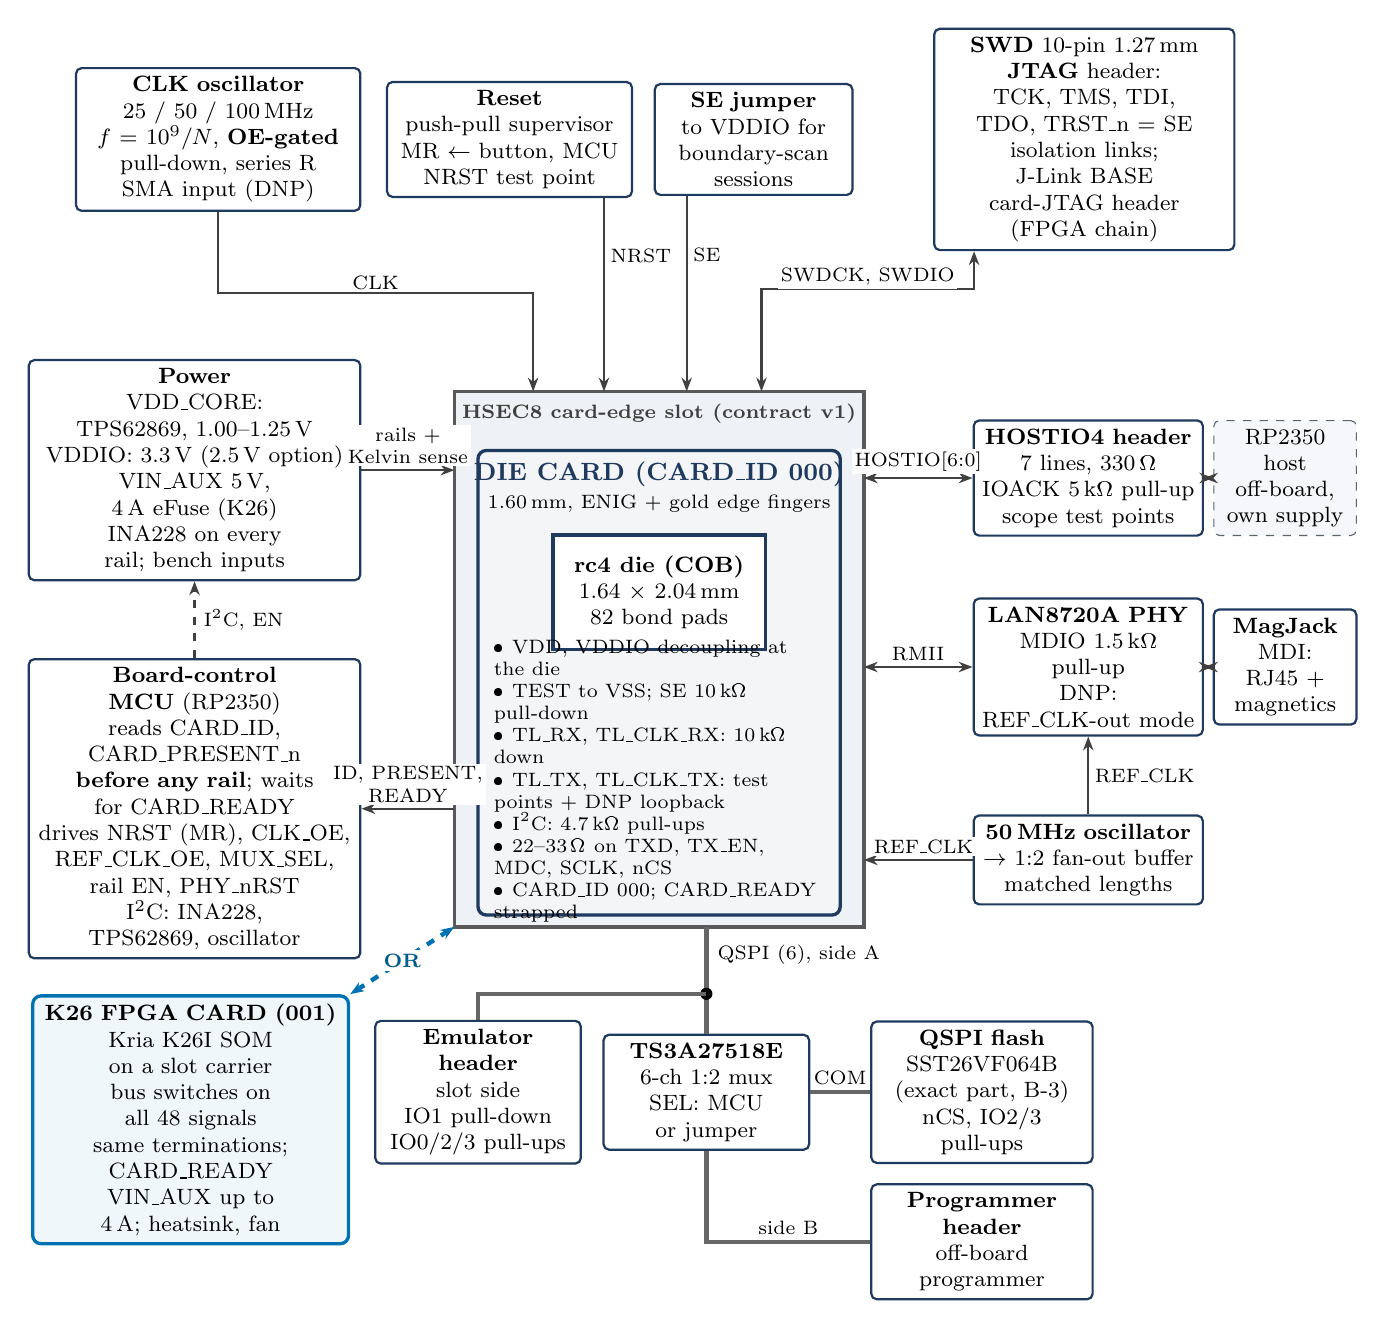
\begin{tikzpicture}[
  font=\footnotesize,
  every node/.append style={execute at begin node=\nohyph},
  blk/.style={draw=accent,thick,rounded corners=2pt,fill=white,align=center,inner sep=3pt,text width=#1},
  blk/.default=3.0cm,
  off/.style={draw=srcgray,dashed,rounded corners=2pt,fill=rowgray,align=center,inner sep=3pt,text width=#1},
  off/.default=1.6cm,
  wire/.style={thick,draw=black!75},
  bus/.style={line width=1.6pt,draw=black!60},
  lab/.style={font=\scriptsize,fill=white,inner sep=1pt},
  >={Stealth[length=5pt]}]
% ---- slot and die card
\node[draw=black!65,line width=1.3pt,fill=headgray!60,minimum width=5.2cm,minimum height=6.8cm] (slot) at (0,-0.2) {};
\node[font=\scriptsize\bfseries,text=black!75] at (0,2.92) {HSEC8 card-edge slot (contract v1)};
\node[draw=accent,line width=1.2pt,fill=accent!5,rounded corners=3pt,minimum width=4.6cm,minimum height=5.9cm] (card) at (0,-0.5) {};
\node[font=\small\bfseries,text=accent] at (0,2.15) {DIE CARD (CARD\_ID 000)};
\node[font=\scriptsize] at (0,1.78) {1.60\,mm, ENIG + gold edge fingers};
\node[draw=accent,line width=1.3pt,fill=white,minimum width=2.7cm,minimum height=1.45cm,align=center] (die) at (0,0.65) {\textbf{rc4 die (COB)}\\ 1.64 $\times$ 2.04\,mm\\ 82 bond pads};
\node[font=\scriptsize,align=left,text width=4.2cm] at (0,-1.75) {%
\textbullet{} VDD, VDDIO decoupling at the die\\
\textbullet{} TEST to VSS; SE 10\,k\textohm{} pull-down\\
\textbullet{} TL\_RX, TL\_CLK\_RX: 10\,k\textohm{} down\\
\textbullet{} TL\_TX, TL\_CLK\_TX: test points + DNP loopback\\
\textbullet{} I\textsuperscript{2}C: 4.7\,k\textohm{} pull-ups\\
\textbullet{} 22--33\,\textohm{} on TXD, TX\_EN, MDC, SCLK, nCS\\
\textbullet{} CARD\_ID 000; CARD\_READY strapped};
% ---- top row (motherboard)
\coordinate (xrst) at (-0.7,0); \coordinate (xse) at (0.35,0); \coordinate (xdbg) at (4.0,0);
\node[blk=3.4cm] (clk) at (-5.6,6.4) {\textbf{CLK oscillator}\\ 25 / 50 / 100\,MHz\\ $f=10^9/N$, \textbf{OE-gated}\\ pull-down, series R\\ SMA input (DNP)};
\node[blk=2.9cm] (rst) at (-1.9,6.4) {\textbf{Reset}\\ push-pull supervisor\\ MR $\leftarrow$ button, MCU\\ NRST test point};
\node[blk=2.3cm] (sej) at (1.2,6.4) {\textbf{SE jumper}\\ to VDDIO for boundary-scan sessions};
\node[blk=3.6cm] (dbg) at (5.4,6.4) {\textbf{SWD} 10-pin 1.27\,mm\\ \textbf{JTAG} header: TCK, TMS, TDI, TDO, TRST\_n = SE\\ isolation links; J-Link BASE\\ card-JTAG header (FPGA chain)};
\draw[wire,->] (clk.south) -- (-5.6,4.45) -- (-1.6,4.45) -- (-1.6,3.2);
\node[lab,above] at (-3.6,4.45) {CLK};
\draw[wire,->] (rst.south -| xrst) -- (-0.7,3.2) node[pos=0.3,lab,right=1pt] {NRST};
\draw[wire,->] (sej.south -| xse) -- (0.35,3.2) node[pos=0.3,lab,right=1pt] {SE};
\draw[wire,<->] (dbg.south -| xdbg) -- (4.0,4.5) -- (1.3,4.5) -- (1.3,3.2);
\node[lab,above] at (2.65,4.5) {SWDCK, SWDIO};
% ---- right column
\node[blk=2.7cm] (hio) at (5.45,2.1) {\textbf{HOSTIO4 header}\\ 7 lines, 330\,\textohm{}\\ IOACK 5\,k\textohm{} pull-up\\ scope test points};
\node[off=1.6cm] (rp) at (7.95,2.1) {RP2350 host\\ off-board,\\ own supply};
\node[blk=2.7cm] (phy) at (5.45,-0.3) {\textbf{LAN8720A PHY}\\ MDIO 1.5\,k\textohm{} pull-up\\ DNP: REF\_CLK-out mode};
\node[blk=1.6cm] (mag) at (7.95,-0.3) {\textbf{MagJack}\\ MDI: RJ45 +\\ magnetics};
\node[blk=2.7cm] (ref) at (5.45,-2.75) {\textbf{50\,MHz oscillator}\\ $\to$ 1:2 fan-out buffer\\ matched lengths};
\draw[wire,<->] (hio.west) -- (2.6,2.1) node[pos=0.5,lab,above=1pt] {HOSTIO[6:0]};
\draw[wire,<->] (hio.east) -- (rp.west);
\draw[wire,<->] (phy.west) -- (2.6,-0.3) node[pos=0.5,lab,above=1pt] {RMII};
\draw[wire,<->] (phy.east) -- (mag.west);
\draw[wire,->] (ref.north) -- (phy.south) node[pos=0.5,lab,right=1pt] {REF\_CLK};
\draw[wire,->] (ref.west) -- (2.6,-2.75) node[pos=0.45,lab,above=1pt] {REF\_CLK};
% ---- left column
\node[blk=4.0cm] (pwr) at (-5.9,2.2) {\textbf{Power}\\ VDD\_CORE: TPS62869, 1.00--1.25\,V\\ VDDIO: 3.3\,V (2.5\,V option)\\ VIN\_AUX 5\,V, 4\,A eFuse (K26)\\ INA228 on every rail; bench inputs};
\draw[wire,->] (pwr.east) -- (-2.6,2.2) node[pos=0.5,lab,above=1pt,align=center] {rails +\\ Kelvin sense};
\node[blk=4.0cm] (mcu) at (-5.9,-2.1) {\textbf{Board-control MCU} (RP2350)\\ reads CARD\_ID, CARD\_PRESENT\_n \textbf{before any rail}; waits for CARD\_READY\\ drives NRST (MR), CLK\_OE, REF\_CLK\_OE, MUX\_SEL, rail EN, PHY\_nRST\\ I\textsuperscript{2}C: INA228, TPS62869, oscillator};
\draw[wire,<-] (mcu.east) -- (-2.6,-2.1) node[pos=0.5,lab,above=1pt,align=center] {ID, PRESENT,\\ READY};
\draw[wire,dashed,->] (mcu.north) -- (pwr.south) node[pos=0.5,lab,right=2pt] {I\textsuperscript{2}C, EN};
\node[draw=gDbg,line width=1.2pt,rounded corners=3pt,fill=gDbg!6,align=center,inner sep=3pt,text width=3.8cm] (fpga) at (-5.95,-6.05) {\textbf{K26 FPGA CARD (001)}\\ Kria K26I SOM on a slot carrier\\ bus switches on all 48 signals\\ same terminations; CARD\_READY\\ VIN\_AUX up to 4\,A; heatsink, fan};
\draw[line width=1.6pt,dashed,draw=gDbg,<->] (fpga.north east) -- (-2.6,-3.6) node[pos=0.5,fill=white,inner sep=1.5pt,font=\scriptsize\bfseries,text=gDbg!80!black] {OR};
% ---- bottom: QSPI (motherboard)
\node[blk=2.4cm] (mux) at (0.6,-5.7) {\textbf{TS3A27518E}\\ 6-ch 1:2 mux\\ SEL: MCU or jumper};
\node[blk=2.6cm] (fl) at (4.1,-5.7) {\textbf{QSPI flash}\\ SST26VF064B\\ (exact part, B-3)\\ nCS, IO2/3 pull-ups};
\node[blk=2.6cm] (prog) at (4.1,-7.6) {\textbf{Programmer header}\\ off-board programmer};
\node[blk=2.4cm] (emu) at (-2.3,-5.7) {\textbf{Emulator header}\\ slot side\\ IO1 pull-down\\ IO0/2/3 pull-ups};
\draw[bus] (0.6,-3.6) -- (mux.north);
\node[lab,right] at (0.7,-3.95) {QSPI (6), side A};
\draw[bus] (mux.east) -- (fl.west) node[pos=0.5,lab,above=1pt] {COM};
\draw[bus] (mux.south) |- (prog.west) node[pos=0.75,lab,above=1pt] {side B};
\fill (0.6,-4.45) circle (2.2pt);
\draw[bus] (0.6,-4.45) -- (-2.3,-4.45) -- (emu.north);
\end{tikzpicture}
\caption[Board block diagram]{Board block diagram. The slot (grey frame) takes \textbf{one of two interchangeable cards}: the die card (shown fitted, centre) or the K26 FPGA card (bottom left); an optional packaged-die card (\texttt{010}) is a third. All carry the same terminations and use the same pins. Every other solid box is on the motherboard, which also provides a mechanical support for the heavier FPGA card. Dashed boxes are off-board. Arrows end at the slot because every signal crosses it one-to-one by pad name (Section~\ref{sec:slot}). Thick lines are multi-signal buses; ``DNP'' means placed but not fitted.}
\label{fig:block}
\end{figure}

\subsection{Per-block requirements}
Parts named in the ``Suggested part'' column come from the parts survey; anything marked TBD still needs a part choice. Resistor values the research did not fix are engineering starting points, marked ``(start)''. \textbf{Where}: MB = motherboard, Card = die card. The K26 FPGA card's contents are in the partition table (Section~\ref{sec:partition}).

{\footnotesize
\setlength{\tabcolsep}{4pt}
\begin{longtable}{@{}P{2.1cm}P{0.9cm}P{8.0cm}P{2.5cm}P{2.1cm}@{}}
\toprule
\rowcolor{headgray}[0pt][0pt]\hd{Block} & \hd{Where} & \hd{Requirement} & \hd{Suggested part} & \hd{Source}\\
\midrule
\endfirsthead
\toprule
\rowcolor{headgray}[0pt][0pt]\hd{Block} & \hd{Where} & \hd{Requirement} & \hd{Suggested part} & \hd{Source}\\
\midrule
\endhead
Die site (COB) & Card & Bond all 82 pads. VSS die-attach pad (substrate connection to confirm). One solder-mask opening over the bond area. Glob-top keep-out ring with no parts inside it. Fingers per Section~\ref{sec:cob}. Decoupling for VDD and VDDIO on every die side, just outside the keep-out & Die, epoxy and glob top chosen by the bonder & Section~\ref{sec:cob} \\
Card edge & Card & HSEC8 card edge, 1.60\,mm card, ENIG + gold edge fingers, longer ground fingers. CARD\_ID straps \texttt{000}; CARD\_READY strapped ready; VIN\_AUX and card-JTAG pins not connected. Optional ID EEPROM on CARD\_I2C & Samtec HSEC8 mating edge & Section~\ref{sec:slot} \\
Slot, card detect, mechanics & MB & HSEC8 socket, 120 positions. CARD\_ID[2:0], both CARD\_PRESENT\_n and CARD\_READY pulled up from the MCU's always-on supply (Section~\ref{sec:cardid}). Keep-out volume over the slot and a card guide or standoff/bracket for the K26 card (up to about 100 $\times$ 90\,mm with heatsink and fan). Card-JTAG pins to a header & Samtec HSEC8, 0.8\,mm & research report 06 \\
Core supply VDD\_CORE & MB & 1.00--1.25\,V adjustable in 5\,mV steps over I\textsuperscript{2}C; nominal 1.20\,V. The host tool clamps the setpoint at $\le$ 1.25\,V, because the regulator's own range reaches 1.675\,V. Choose a variant that powers up at $\le$ 1.20\,V. Enabled only for CARD\_ID \texttt{000}/\texttt{010}; optional DNP dummy load to test it with the K26 card fitted. Kelvin sense from the card (\sig{VDD_CORE_SENSE_P/N}). A jumper selects the on-board regulator or a bench-supply input. INA228 on \sig{VDD_DIE} & TPS62869; INA228 & \src{UPF:107-109}; \src{REG:403-405,484-485} \\
IO supply VDDIO & MB & 3.3\,V, on for every card type (the K26 card powers its slot bus switches from it). A 2.5\,V fallback must need only a resistor or regulator change. One regulator with two measured branches: \sig{VDDIO_DIE} (to the slot) and \sig{VDDIO_BOARD} (flash, PHY IO, oscillators, pull-ups). This keeps them at one voltage and one sequence. Kelvin sense from the card (\sig{VDDIO_SENSE_P/N}). INA228 on each branch; jumper to a bench-supply input & TPS7A94 (resistor-set); INA228 & research report 03 \S C3 \\
VIN\_AUX & MB & 5\,V to the slot for the K26 card only (CARD\_ID \texttt{001}): $\ge$ 4\,A continuous on $\ge$ 6 contacts, through an eFuse, with an INA228 & eFuse TBD; INA228 & research report 06 \\
PHY analogue supply & MB & From a fixed 3.3\,V rail, so that only the PHY's VDDIO follows the die VDDIO. Check the PHY datasheet & LAN8720A datasheet & -- \\
CLK & MB & CMOS, full swing at VDDIO, max transition 1.2\,ns at the die, through the connector. 25\,MHz (FPGA builds), \textbf{50\,MHz for the die's boot} (default; B2), 100\,MHz only after firmware sets CLK\_DIV $\ge$ 2; every setting must be $10^9/N$ Hz. OE driven by the host MCU, with a jumper override. Output start after OE must be glitch-free. Pull-down 100\,k\textohm{} (start) on the slot side so CLK rests low while the oscillator output is disabled. Series 22--33\,\textohm{} at the source. DNP SMA for an external generator (shmoo). Test point next to the slot & TBD: programmable oscillator, or 25, 50 and 100\,MHz parts with OE & \src{SDC:12,66-67}; \src{PROC:190-203} \\
Reset & MB & Push-pull, active-low supervisor output on NRST, monitoring VDDIO (and VDD if dual-input). Button and host-MCU open-drain line into MR. Edge $\le$ 5\,ns. Test point & TBD (push-pull output, MR input) & \src{SDC:71-72}; \src{REG:359-377} \\
Straps & Card + MB & Every card: TEST 0\,\textohm{} (or 10\,k\textohm{}) to VSS plus a test point; SE 10\,k\textohm{} pull-down. MB: SE jumper to VDDIO and the JTAG header's TRST\_n pin & -- & \src{PROC:204-220} \\
QSPI flash & MB & Accepts \texttt{0x0B} (fast read, 8 dummy clocks), \texttt{0x06}, \texttt{0x02}, \texttt{0x05} and ULBPR \texttt{0x98}. 3-byte addressing; keep the image under 4\,MB. The mux common side goes to the flash, side A to the slot, side B to a programmer header; SEL from the host MCU plus a jumper, default A. Emulator header on the slot side. Slot side: IO1 pull-down 10\,k\textohm{}, IO0/IO2/IO3 pull-ups 47\,k\textohm{} (start). Flash side: nCS, IO2, IO3 pull-ups 10\,k\textohm{}. SCLK/nCS series resistors sit on the card; series-R footprints and scope points on SCLK, IO0 and IO1 at the die (B-5) & SST26VF064B (3.3\,V), exact part (B-3); TS3A27518E & \src{ROM1:18,119,259-267}; \src{REG:242-266} \\
Ethernet & MB & LAN8720A in REF\_CLK-in mode, fed by the fan-out buffer. DNP 0\,\textohm{} and a DNP 25\,MHz crystal for REF\_CLK-out mode (strap \sig{nINTSEL}=0, which shares the LED2 pin and flips its polarity). MDIO 1.5\,k\textohm{} pull-up. TXD0/1, TX\_EN, MDC series resistors sit on the card. PHY reset from the host MCU. Record the PHY address straps. Human-routed 100\,\textohm{} MDI pairs to the MagJack & LAN8720A; MagJack; 1:2 fan-out buffer TBD & \src{docs/bringup/KR260_LAN8720_FPGAHUB_PLAN.md:4}; \src{HFW:74-94} \\
REF\_CLK & MB & 50\,MHz oscillator with OE (host MCU) into the fan-out buffer. Length-matched branches to the PHY and, through the slot, to \sig{RMII_REF_CLK}; count the card trace in the match. Weak pull-down on the slot side & TBD & \src{SDC:13,35-36} \\
HOSTIO4 header & MB & 7 signals plus ground; \textbf{no power pin}, because back-feeding the host's 3V3 is forbidden. Pin order \sig{HOSTIO[n]} = RP2350 GP$n$, $n$ = 0..6; this is the reference PIO driver's order, so confirm it against the bench build. 330\,\textohm{} series on the host side of the isolation links. IOACK pull-up about 5\,k\textohm{} and 10\,k\textohm{} idle pull-ups on the other six, on the slot side of the 330\,\textohm. Scope test points on IOACK and IOREQ1 & Waveshare RP2350 (off-board) & \src{PROC:163-246}; \src{hostio-pio.py:7-11} \\
SWD header & MB & Arm 10-pin 1.27\,mm Cortex debug layout. VTref = VDDIO; SWDIO and SWCLK with 22--33\,\textohm{} series. nRESET to the supervisor MR through a DNP link. Isolation links to the JTAG header & J-Link BASE (1.2--5\,V) & \src{XDBG:54-62} \\
JTAG (boundary scan) & MB & TCK=\sig{SWDCK}, TMS=\sig{SWDIO}, TDI=\sig{HOSTIO[0]}, TDO=\sig{HOSTIO[1]}, TRST\_n=\sig{SE}, VTref, GND. Links make \{HOSTIO header, JTAG\} exclusive on \sig{HOSTIO[0:1]} and \{SWD, JTAG\} exclusive on \sig{SWDCK}/\sig{SWDIO} (Table~\ref{tab:links}). Any J-Link-compatible connector that carries TRST & J-Link BASE; OpenOCD SVF & \src{BSC:77-95}; \src{PTAB} \\
Board-control MCU & MB & Reads CARD\_ID and CARD\_PRESENT\_n before any rail, and waits for CARD\_READY before NRST. Drives NRST (through MR), CLK\_OE, REF\_CLK\_OE, MUX\_SEL, EN\_VDD, EN\_VDDIO, EN\_VIN\_AUX and PHY\_nRST. I\textsuperscript{2}C master for the INA228s, the TPS62869 and a programmable oscillator. Its I\textsuperscript{2}C bus must stay separate from the die's \sig{I2C_SCL/SDA}. It can be the HOSTIO RP2350 or a second one on a control header & RP2350 (on a header) & -- \\
TideLink park & Card & See Section~\ref{sec:tlpark}. The 18 TL signals also reach the slot; the single-slot motherboard leaves them unconnected & -- & \src{BSC:455-476} \\
Current monitors & MB & INA228 on \sig{VDD_DIE}, \sig{VDDIO_DIE}, \sig{VDDIO_BOARD} and \sig{VIN_AUX} (size that shunt for $\ge$ 4\,A); optional on 3V3\_AUX. Size each shunt so about 250\,mA is full scale (start). Log energy and charge per phase & INA228 & research report 03 \S C3 \\
\bottomrule
\end{longtable}\addtocounter{table}{-1}}

\subsection{Power}\label{sec:power}
{\footnotesize
\setlength{\tabcolsep}{4pt}
\begin{longtable}{@{}P{1.8cm}P{1.25cm}P{2.2cm}P{2.3cm}P{4.4cm}P{1.4cm}P{1.2cm}@{}}
\toprule
\rowcolor{headgray}[0pt][0pt]\hd{Rail} & \hd{Nominal} & \hd{Range on board} & \hd{Die pads} & \hd{Expected current} & \hd{First-power limit (start)} & \hd{Monitor}\\
\midrule
\endhead
\sig{VDD_DIE} (slot \sig{VDD_CORE}) & 1.20\,V & 1.00--1.25\,V, 5\,mV steps, Kelvin-sensed at the card. \textbf{Never 1.32\,V} & 6 $\times$ VDD, 4 $\times$ VSS (top and bottom) & $\le$ 50.7\,mA (default-toggle estimate, 1.08\,V SS, fp1505). Real workloads 7.4--8.3\,mW at 50\,MHz, 15.0\,mW (about 14\,mA) at 100\,MHz. Leakage 0.36\,mW (SS, 125\,\textdegree C). 7.9--13.1\,mA per core pad measured in rail analysis & 100\,mA & INA228 \\
\sig{VDDIO_DIE} & 3.3\,V & 3.3\,V; 2.5\,V fallback & 12 $\times$ VDDIO (1 POC), 12 $\times$ VSSIO & \NF. The IO ring was never analysed & 50\,mA & INA228 \\
\sig{VDDIO_BOARD} & = VDDIO & same regulator & -- & Per the part datasheets (flash, PHY IO, oscillators, pull-ups) & -- & INA228 \\
\sig{VIN_AUX} & 5\,V & fixed, eFuse & -- (K26 card only; $\ge$ 6 contacts) & Up to about 4\,A for the K26 card; design for $\ge$ 4\,A continuous & eFuse & INA228 \\
3V3\_AUX & 3.3\,V & fixed & -- & PHY analogue, board MCU if on-board & -- & optional \\
\bottomrule
\end{longtable}\addtocounter{table}{-1}}
{\raggedright\scriptsize\color{srcgray} Sources: \src{docs/tapeout/31-power-delivery-measured.md:814-816,839-853,956}; \src{ASIC/eth-chiplet/build/power-saif-20260827/SUMMARY.txt:20-25}; \src{docs/tapeout/32-ir-drop-stage.md:802-810}.\par}

\textbf{Sequencing.} POC behaviour and power-sequencing rules are \NF{} (open question 2). The rule \src{REG:473-477} gives for bring-up is: diode-check every pin, then measure IO supply current \emph{before} applying core power. Every power-up therefore follows this standard sequence, S1, which the board-control script implements:
\begin{enumerate}
\setcounter{enumi}{-1}
\item Card check (Section~\ref{sec:cardid}): both \sig{CARD_PRESENT_n} low and \sig{CARD_ID} = \texttt{000} (or \texttt{010}). Otherwise stop: no rail is enabled. (The K26 card follows the same rule with its own rails: VDDIO and VIN\_AUX, never VDD\_CORE.)
\item CLK\_OE = 0, REF\_CLK\_OE = 0, NRST held low (MR asserted), flash mux on side A, HOSTIO host outputs Hi-Z or host unplugged.
\item Enable \sig{VDDIO} (current-limited). Wait for the INA228 reading to settle and record \sig{VDDIO_DIE} current with VDD off. Keep this step short: what the POC does with the core unpowered is not known.
\item Enable \sig{VDD} at 1.20\,V (first time only: ramp in 0.1\,V steps and record the current at each step). Record \sig{VDD_DIE} current.
\item REF\_CLK\_OE = 1. Only now enable the HOSTIO host's pins or plug in the probe. The 330\,\textohm{} series resistors limit injection current if this order is broken.
\item Start the HOSTIO capture (HIO-001 needs the cold-boot banner).
\item Check \sig{CARD_READY} (strapped ready on the die card; on the K26 card it follows configuration). Then release NRST with CLK \textbf{stopped} (erratum N1). Wait at least the supervisor timeout plus 10\,ms.
\item CLK\_OE = 1. Reset releases synchronously a few CLK edges later; the ROMs start.
\end{enumerate}
Power-down reverses the order: CLK\_OE = 0, NRST low, VDD off, VDDIO off. Only then may a card be removed or inserted.

\subsection{Clocking}
There is no PLL: the board oscillator \emph{is} the fabric clock. The motherboard oscillator offers 25, 50 and 100\,MHz (contract v1). Everything time-derived follows it: PHC \sig{NS_INCR}, the QSPI boot clock (SCLK = CLK/2, because \sig{CLK_DIV} resets to 1 and neither ROM writes it), the XiP no-flash watchdog ($65536/f$), timer reloads, and the firmware's \sig{FW_CORE_HZ}.

{\small
\begin{longtable}{@{}P{1.9cm}P{2.2cm}P{2.4cm}P{2.0cm}P{6.4cm}@{}}
\toprule
\rowcolor{headgray}[0pt][0pt]\hd{CLK} & \hd{\sig{NS_INCR} = $10^9/f$} & \hd{QSPI SCLK at boot} & \hd{XiP watchdog} & \hd{Use}\\
\midrule
\endhead
25.0\,MHz & 40 & 12.5\,MHz & 2.62\,ms & \textbf{Option (contract v1):} the rate every FPGA build runs at; K26 card in Phase M, and a slow point for the die \\
50.0\,MHz & 20 & 25\,MHz & 1.31\,ms & \textbf{Default and boot clock.} Flash read $+5.0$\,ns at SS with CLK\_DIV = 1 (B2) \\
62.5\,MHz & 16 & 31.25\,MHz & 1.05\,ms & Shmoo step \\
83.3\,MHz & 12 & 41.7\,MHz & 0.79\,ms & Shmoo step \\
90.9\,MHz & 11 & 45.5\,MHz & 0.72\,ms & About the slow-part limit ($\approx$95\,MHz at SS/cworst, item 6f). Flash read \textbf{fails} at CLK\_DIV = 1 ($-4.0$\,ns SS) \\
100.0\,MHz & 10 & 50\,MHz & 0.655\,ms & SDC target. Flash read \textbf{fails} at CLK\_DIV = 1 ($-5.0$\,ns SS): firmware sets CLK\_DIV $\ge$ 2 before CLK is raised \\
\bottomrule
\end{longtable}\addtocounter{table}{-1}}
\begin{itemize}
\item \textbf{RMII\_REF\_CLK} is a 50\,MHz \emph{input}; the MII clocks are generated on the die at $\div$2 \src{SDC:13,35-36}.
\item \textbf{SWDCK} is constrained to 25\,MHz \src{SDC:14}. Start \textbf{boundary-scan TCK} at about 1\,MHz \src{BSC:134-138}.
\item The \textbf{TideLink link clock} is fixed at /1 and gated while ROLE\_CFG is unwritten, which it always is on this board \src{REG:151-153}.
\item The PHC \sig{NS_INCR_FRAC} field is signed, and the procedure's FRAC formula is wrong when the fraction is 0.5 or more. That is the reason every frequency is $10^9/N$ \src{NMS/ptp-hardware-clock-ahb/src/rtl/phc_clock_core.sv:132-156}.
\end{itemize}

\subsection{Reset}
\begin{itemize}
\item NRST asserts asynchronously and releases synchronously on CLK into \sig{SYS_PORESETn}/\sig{HRESETn}, so \textbf{CLK must run for reset to release} \src{PRMU:133-157}.
\item \textbf{Erratum N1.} Raw NRST also resets about 4,027 flops asynchronously, with no synchroniser: the PHC (899 flops) and the debug group. Releasing NRST with CLK stopped, as in sequence S1 step 6, is advised, not mandatory: with CLK running, STA puts 65--69\,\% of release phases at SS on a removal check, but every affected flop is benign \src{docs/chip-reference-manual/review/closure/item06-sta.md} \S6a. Clear the perf counters and ETC and re-initialise the PHC after boot \src{REG:359-377}.
\item The TideLink role lock clears only on power-on reset, i.e.\ NRST.
\item Software resets live at \texttt{0x2A000020}. Bit 0 is \sig{CPU0_SWRST}. Bit 1 is \sig{CPU1_SWRST}, which resets the whole fabric \emph{including HOSTIO}, so the link drops and must be re-entered \src{PROC:848}; \src{REG:280}.
\end{itemize}

\subsection{Debug headers and isolation links}\label{sec:links}
Boundary scan and HOSTIO are mutually exclusive, and boundary scan shares its pins with SWD. Each bench session fits exactly one link set:

\begin{table}[H]
\centering\small
\begin{tabularx}{\textwidth}{@{}P{3.3cm}P{2.0cm}P{2.0cm}P{2.0cm}P{1.8cm}L@{}}
\toprule
\rowcolor{headgray}[0pt][0pt]\hd{Session} & \hd{HOSTIO[0:1] $\to$ HOSTIO hdr} & \hd{HOSTIO[0:1] $\to$ JTAG hdr} & \hd{SWD pins $\to$ JTAG hdr} & \hd{SE} & \hd{Notes}\\
\midrule
HOSTIO (P3--P7, P9--P15) & fitted & open & open & low & SWD header may stay connected (P8), subject to the two-master rule \\
SWD (P8) & fitted & open & open & low & SWD pins go to the SWD header \\
Boundary scan (P2) & \textbf{open} & fitted & fitted & \textbf{high (last)} & NRST low; HOSTIO host unplugged. Raise SE \emph{before} driving TDI, or TDI fights a 16\,mA driver \src{BSC:20-40} \\
\bottomrule
\end{tabularx}
\caption[Isolation-link settings]{Isolation-link settings per session. ``fitted'' means the 0\,\textohm{} link or jumper is in place.}
\label{tab:links}
\end{table}

\subsection{TideLink parking (on the die card)}\label{sec:tlpark}
All parking parts sit on the die card; the 18 TL signals and the I\textsuperscript{2}C pair also reach the slot, so a later two-slot motherboard can join two dies, but the single-slot motherboard leaves them unconnected. The die cannot toggle these pins on its own. rc4 is built with \sig{NEGO_CFG_RESET0}, \sig{SELF_ARM_TRAIN_EN1}, \sig{AUTO_ANCHOR_EN1} and \sig{ROLE_FROM_STRAP1}. Nothing on the die writes ROLE\_CFG. While ROLE\_CFG is unwritten, \sig{wlink_por_reset} holds the link in reset and \sig{pad_clk_tx} stays gated. The TX pads still drive a static level, but that level is not established \src{REG:78-98}.
\begin{itemize}
\item \textbf{TL\_RX[7:0], TL\_CLK\_RX}: bond them, and pull each to VSSIO with 10\,k\textohm. They have no keeper.
\item \textbf{TL\_TX[7:0], TL\_CLK\_TX}: bond them (B-1) to test points and to the loopback footprints. They cannot be tri-stated and must never touch a rail.
\item \textbf{Loopback footprints (B-1)}: DNP 0\,\textohm{} \sig{TL_TX[n]}$\to$\sig{TL_RX[n]} and \sig{TL_CLK_TX}$\to$\sig{TL_CLK_RX}, next to the die and length-matched, keeping the 10\,k\textohm{} pull-downs. With them fitted, boundary-scan continuity of all nine lanes runs from the TAP alone (\sig{p2_extest_walk_tlloop.svf}), and after one ROLE\_CFG write the die trains the shipped V2/CRC/ECC/8-lane configuration against itself through real pads at real CLK (P2b). This is the only silicon measurement of the D2D link possible before a compute die and a pair board exist \src{docs/chip-reference-manual/review/closure/item03-d2d-loopback.md}. In ring order the clock sits mid-bus: \sig{TL_CLK_TX} is between TX[4] and TX[3], and \sig{TL_CLK_RX} between RX[4] and RX[3] \src{BSC:450-476}.
\item \textbf{I\textsuperscript{2}C\_SCL/SDA}: 4.7\,k\textohm{} to VDDIO on the card (the contract's value; 2.2--4.7\,k\textohm{} is acceptable), plus test points. The pad comment says real 2.2\,k pull-ups belong on the PCB \src{PADS:926-932}.
\item \textbf{Firmware and tools}: never write ROLE\_CFG \texttt{0x2E032080}, except in P2b with the loopback fitted. Link status at \texttt{0x2E032084} is safe to read with the link down \src{docs/design/PIN_MAP.md:196-210}.
\end{itemize}

\subsection{Die-card chip-on-board footprint and bonding rules}\label{sec:cob}
These rules apply to the \textbf{die card} only. The motherboard needs no bondable finish and can come from any fab.

\textbf{Settle the bonder's rules before the card layout.} Zepler Cleanrooms (on campus) has a manual Au/Al wire bonder, dicing and die bonders. Its model and pad limits are unconfirmed; one search snippet describes a campus ``5430 Fine Wire Bonder'' as an ultrasonic \emph{wedge} bonder (25\,\textmu m wire, 50 $\times$ 50\,\textmu m minimum pads), which would mean Al wedge and ENIG. Custom Interconnect Ltd (Andover) is the nearest outsourced house.

{\footnotesize
\setlength{\tabcolsep}{4pt}
\begin{longtable}{@{}P{3.0cm}P{9.8cm}P{3.6cm}@{}}
\toprule
\rowcolor{headgray}[0pt][0pt]\hd{Rule} & \hd{Value} & \hd{Source}\\
\midrule
\endfirsthead
\toprule
\rowcolor{headgray}[0pt][0pt]\hd{Rule} & \hd{Value} & \hd{Source}\\
\midrule
\endhead
Wire and card finish & Al wedge (ultrasonic, unheated) works on \textbf{ENIG}: order the card as \textbf{ENIG + gold edge fingers} (Eurocircuits offers selective ENIG with a gold-edge-connector option). Au ball (thermosonic, heated substrate) needs \textbf{ENEPIG}; ENEPIG plus hard-gold fingers on one card is \textbf{unconfirmed} (PCBWay lists both, not together). The bonder decides & Würth webinar 108; JLCPCB ENEPIG vs ENIG; research report 05 \S4 \\
Card fits the bonder & \textbf{Check:} the card must fit the bonder's stage and clamp, and its heated stage if Au ball. An HB16-class manual bonder takes samples up to 100 $\times$ 150\,mm [search snippet]; confirm Zepler's limit and any thickness limit against the 1.60\,mm card HSEC8 needs & research report 05 \S4; Technion HB16 page \\
Bond finger & $\ge$ 150\,\textmu m wide, 300\,\textmu m long; $\ge$ 100\,\textmu m between fingers ($\ge$ 250\,\textmu m pitch) & Würth design-rule poster v1.2 \\
Die edge to finger & $\ge$ 1.5 $\times$ die thickness (thickness \NF) & Würth poster \\
Solder mask & One opening over the whole bond area & Würth poster \\
Wire length & 25\,\textmu m Au $\le$ 6\,mm (17.5\,\textmu m $\le$ 4.5\,mm; 33\,\textmu m $\le$ 7\,mm) & Europractice packaging rules 2024 \\
Wire angle & $\le$ 45\textdegree{} from the pad normal. \textbf{No crossing wires} & Europractice 2024 \\
Die pad & Opening $\ge$ 55 $\times$ 55\,\textmu m and pitch $\ge$ 65\,\textmu m. This die has 58 $\times$ 66\,\textmu m and 67/80\,\textmu m alternating & Europractice 2024; \src{REG:500-502} \\
Staggered rows & The P60 bond rules were never run (imec ran P80). The bonder must confirm its capillary and loop plan for 134/160\,\textmu m same-row pitch with a 102\,\textmu m row offset & \src{REG:500-502}; \src{docs/tapeout/60-waiver-document-rc1v3r4.md:158-175} \\
Die placement & $\pm$100\,\textmu m (manual) & Europractice 2024 \\
Die attach & Conductive epoxy (H20E) to a VSS copper pad with the finish on it. Non-conductive epoxy (H70E) needs explicit ground bonds. Substrate and backside connection to confirm with imec & Europractice 2024 \\
Glob top & Full, spot or dam-and-fill. Keep the keep-out ring free of parts and test points & Würth webinar \\
Fiducials & Not sourced; ask the bonder. Bonders usually photograph the die to find it & KiCad forum \\
\bottomrule
\end{longtable}\addtocounter{table}{-1}}

\textbf{Fan-out feasibility.} Table~\ref{tab:fanout} is a first check against these rules, computed by \sig{figures/gen_figs.py}. Assumptions: one finger row at 250\,\textmu m pitch, centred on each die edge; distances measured from the seal-ring edge; each wire runs from the opening centre to the finger centre. The \textbf{left (D2D) edge governs}. A single rectangular finger ring at least 2.23\,mm from the seal ring keeps every wire within 45\textdegree{} and under 3.4\,mm long, inside the 6\,mm limit. The left row's ends then overhang the die by 2.18\,mm but stay clear of the top and bottom rows.

\begin{table}[H]
\centering\small
\begin{tabular}{@{}lcccccc@{}}
\toprule
\rowcolor{headgray}[0pt][0pt]\hd{Edge} & \hd{Pads} & \hd{Die edge} & \hd{Finger row} & \hd{Overhang / side} & \hd{Min.\ offset for 45\textdegree} & \hd{Wire length at 2.23\,mm}\\
 & & (mm) & (mm) & (mm) & (mm) & (mm)\\
\midrule
Left & 26 & 2.04 & 6.40 & 2.18 & 2.23 & 2.3--3.3 \\
Top & 17 & 1.64 & 4.15 & 1.25 & 1.31 & 2.3--2.7 \\
Right & 22 & 2.04 & 5.40 & 1.68 & 1.73 & 2.3--3.0 \\
Bottom & 17 & 1.64 & 4.15 & 1.25 & 1.31 & 2.3--2.7 \\
% common ring offset for 45 deg on every edge: 2.23 mm

\bottomrule
\end{tabular}
\caption[Fan-out estimate]{Single-row fan-out estimate. The sawn edge lies beyond the seal ring by the scribe width, which is \NF; add it to every offset.}
\label{tab:fanout}
\end{table}

If the bonder wants shorter wires or a tighter angle, there are three options: two staggered finger rows; leaving \sig{TL_TX[7:0]}/\sig{TL_CLK_TX} unbonded (nine fewer left-edge wires, but no loopback and no P2b; rejected by B-1); or a finer finger pitch, if the bonder allows it.

\textbf{Footprint generator.} KiCad has no wire-bond object. Generate the footprint with a script from the pad CSV:
\begin{itemize}
\item Place the die pads at the \textbf{opening centres}, not the CSV centres. The CSV centre is the pad \emph{cell} centre. Openings sit 36.8\,\textmu m (outer row) or 138.8\,\textmu m (inner row) from the design-frame edge; the seal-ring frame adds 20\,\textmu m. Appendix~\ref{app:pads} lists every opening.
\item Correct the CSV edge label of \sig{BuPAD_HOST_IO_6} from top to \textbf{right}.
\item Emit: die outline and pads on a fab/documentation layer; fingers on F.Cu named by net; the VSS die-attach pad; the glob-top keep-out on a user layer; one solder-mask opening.
\item Check: angle $\le$ 45\textdegree, length $\le$ 6\,mm, no crossings, finger spacing $\ge$ 100\,\textmu m, die-to-finger $\ge$ 1.5 $\times$ thickness.
\item Export a bonding diagram (pad, net, finger, wire length and angle) for Zepler.
\end{itemize}

\textbf{Hedge.} Package about 10 dies through Europractice in parallel with 2--3 COB die cards, and mount them on packaged-die cards (CARD\_ID \texttt{010}) in the same slot. Cost: €485 setup per bonding diagram, QFN Open-Pak €83--€229 per unit, so 10 in QFN $\approx$ €1.3k--2.8k. QFN needs dies $\le$ 300\,\textmu m thick (Open-Pak $\le$ 280\,\textmu m), so thinning may be needed; ceramic takes up to 600\,\textmu m. Lead time is not confirmed (up to 6 weeks in one search snippet). A bad COB die or bond scraps one small card; the motherboard is reused.

\subsection{Test points}
{\small
\begin{longtable}{@{}P{3.6cm}P{1.0cm}P{4.1cm}P{6.9cm}@{}}
\toprule
\rowcolor{headgray}[0pt][0pt]\hd{Test point(s)} & \hd{Where} & \hd{Net} & \hd{Purpose}\\
\midrule
\endhead
\sig{TP_VDD_T}, \sig{TP_VDD_B} & Card & VDD at the top and bottom fingers & Rail voltage at the die (Kelvin), for the shmoo \\
\sig{TP_VDDIO_x} & Card & VDDIO, one per side & IO rail at the die \\
\sig{TP_GND} $\times$ $\ge$ 6 & both & VSS/VSSIO & Scope ground springs next to every signal test point group \\
\sig{TP_CLK} & MB & \sig{CLK}, slot side of the series R & Frequency; edges $\le$ 1.2\,ns; clean start after OE \\
\sig{TP_REFCLK} & MB & \sig{RMII_REF_CLK}, slot side & 50\,MHz present \\
\sig{TP_NRST} & MB & \sig{NRST} & Release timing against CLK (N1) \\
\sig{TP_SE}, \sig{TP_TEST} & Card & straps & Level check at the start of every session \\
\sig{TP_IOACK}, \sig{TP_IOREQ1} & MB & \sig{HOSTIO[2]}, \sig{HOSTIO[0]} & \textbf{Mandatory} scope points: the only way to split ``SoC never requested'' from ``host never acknowledged'' \src{PROC:188} \\
\sig{TP_QSPI_x} $\times$4 & MB & \sig{QSPI_SCLK}, \sig{nCS}, \sig{IO0}, \sig{IO1} & Boot activity after NRST release; SCLK = CLK/2. B-5: also scope points at the die on SCLK, IO0, IO1 for the capture margin \\
\sig{TP_MDC}, \sig{TP_MDIO} & MB & RMII management & MDIO pull-up level; MDC rate \\
\sig{TP_TXEN}, \sig{TP_CRSDV} & MB & RMII & Frame activity \\
\sig{TP_TL_TX[7:0]}, \sig{TP_TL_CLK_TX} & Card & TideLink outputs & Static level; EXTEST continuity. Unloaded otherwise \\
\sig{TP_SCL}, \sig{TP_SDA} & Card & die I\textsuperscript{2}C & Pull-up level \\
\sig{TP_CARD_ID}, \sig{TP_PRESENT}, \sig{TP_CARD_READY} & MB & card detect & CARD\_ID, mating and ready checks \\
\sig{TP_VIN_AUX} & MB & VIN\_AUX after the eFuse & K26 card supply \\
\sig{TP_CLK_OE}, \sig{TP_MUX_SEL}, \sig{TP_EN_x} & MB & board control & Sequencing checks \\
\bottomrule
\end{longtable}\addtocounter{table}{-1}}

\subsection{PCB tooling}
\begin{itemize}
\item \textbf{Flow:} SKiDL (Python; MIT; v2.3.0, 2026-07) or Diode Zener (\sig{pcb} CLI) for the schematic and netlist $\to$ KiCad 10 $\to$ \cmd{kicad-cli sch erc} and \cmd{kicad-cli pcb drc --format json --exit-code-violations} in a loop that Claude fixes $\to$ Freerouting (CLI, v2.4.1) for the slow nets $\to$ KiCad/KiKit fab outputs. Two boards: the \textbf{motherboard} from any fab with a standard finish; the \textbf{die card} as ENIG + gold edge fingers (Eurocircuits) for Al wedge, or PCBWay ENEPIG ($\ge$ 2\,\textmu in Au, wire-bond note on the order) for Au ball.
\item \textbf{Claude does:} netlist, straps, BOM, the COB footprint generator, the HSEC8 pinout checker, the ERC/DRC loop, fab outputs.
\item \textbf{A human does:} die and finger placement agreed with the bonder; the RMII, MDI and finger fan-out routing; magnetics placement; stack-up and impedance; final DRC sign-off.
\item \textbf{Estimate} (research report 03): 1--2 days for the schematic, half a day for the footprint generator, 1--2 days for placement, 1--3 days for routing, then hours for DRC and fab outputs.
\end{itemize}
Tool comparisons, fab capabilities and MCP servers belong in a separate report.

\needspace{12\baselineskip}
% =====================================================================
\section{Preparation before first power}\label{sec:prep}
% =====================================================================
\subsection{Bench equipment}
\begin{itemize}
\item Two-channel bench supply with current limit, ESD-safe station, DMM with diode mode, 4-channel oscilloscope with bandwidth well above the 100\,MHz CLK, stereo microscope and camera for bond photographs.
\item The motherboard with its HSEC8 slot; the K26 FPGA card (Phase M, golden reference); the lab KR260s for emulator-bitstream development.
\item J-Link BASE with OpenOCD. A Waveshare RP2350 running MicroPython with the HOSTIO PIO driver. A flash programmer for the off-board header. Optionally an SPI-NOR emulator.
\item A host PC with a spare Ethernet NIC and Wireshark on a private subnet. \sig{apps/eth_ping_responder} answers at \sig{192.168.10.2}.
\item Optional: a thermal camera, and a temperature chamber for P15 (whether one exists is \NF).
\end{itemize}

\subsection{Host tools checklist}
{\footnotesize
\setlength{\tabcolsep}{4pt}
\begin{longtable}{@{}P{0.45cm}P{3.6cm}P{6.0cm}P{4.2cm}P{1.1cm}@{}}
\toprule
\rowcolor{headgray}[0pt][0pt]\hd{\#} & \hd{Item} & \hd{Check before power} & \hd{Path} & \hd{Status}\\
\midrule
\endhead
1 & RP2350 PIO driver & Status-nibble polarity fixed (the reference driver idles it active-low; the RTL expects active-high). \sig{put()} guarded on \cmd{tx_fifo() < 4}. Resync watchdog live & \src{NMS/nanosoc_arch_tech/rtl/hostio4/rpi-pico-pio/pico-mp/hostio-pio.py}; \src{PROC:247-280} & \EX \\
2 & ADP client & First command after ESC is rejected (\sig{adp.enter()} absorbs it). Parameters always \sig{x} + 8 hex digits. Re-issue \sig{A} before every access & \src{RIG/hostio_adp.py} & \EX \\
3 & HOSTIO suite & \cmd{--target asic_tsmc65}; capture to file with the die serial in the name. \sig{golden_asic_reference.json} generated from the rc4-RTL dry run (\sig{build/presilicon-closure/item08/scripts/rig/eth_chiplet/hostio_suite/golden_asic_reference.json}, sha256 \texttt{98fcaa91}\ldots); place it in the repo & \src{RIG/hostio_suite}; \src{docs/chip-reference-manual/review/closure/item08-bringup-dryrun.md} & \PA \\
4 & Board-control script & Card check (CARD\_ID, PRESENT) before any rail; wait for CARD\_READY before NRST; sequence S1; INA228 logging; TPS62869 setpoint clamp $\le$ 1.25\,V; CLK\_OE, NRST, MUX\_SEL. Proven in Phase M & -- & \NW \\
5 & Address blocklist & Enforced in the client (refuses listed addresses); Appendix~\ref{app:blocklist} & -- & \NW \\
6 & Flash programming flow & Programmer + mux control + read-back verify + sha256 logged & -- & \NW \\
7 & Boundary-scan script & IDCODE, BYPASS, SAMPLE/PRELOAD, EXTEST from the BSDL & \src{sys_desc/bscan/nanosoc_eth_chiplet_pads.bsdl} & \NW \\
8 & SWD OpenOCD config & Manual AP setup (no ROM table); JTAG-to-SWD switch & FPGA reference \src{docs/bringup/KR260_BOARD_WIRING.md:82} & \NW \\
\bottomrule
\end{longtable}\addtocounter{table}{-1}}

\subsection{Flash images}\label{sec:images}
Pack every image with \sig{flash_pack.py} and validate it with \sig{check_flash.py}, which checks the ROMs' own accept and reject rules. Log the sha256 of every image programmed.

{\footnotesize
\setlength{\tabcolsep}{4pt}
\begin{longtable}{@{}P{1.2cm}P{4.2cm}P{4.2cm}P{6.4cm}@{}}
\toprule
\rowcolor{headgray}[0pt][0pt]\hd{Image} & \hd{CPU1 (entry 1, slot A 0x30000)} & \hd{CPU0 (entry 0, 0x60000)} & \hd{Purpose / expected signature}\\
\midrule
\endhead
IMG-0 & -- (erased device) & -- & P4 boot autopsy with blank flash. Ladder rung 6 = \texttt{0x4} \\
IMG-1 & Minimal CPU1 image or the CPU1 shim. It must \textbf{not} write \texttt{0x2D000000--0x2D00004F} or \texttt{0x2D001FF0} & \sig{hostio_fw/fw_heartbeat} built with \sig{TARGET=asic}, \sig{FW_CORE_HZ} = board CLK & P11. \texttt{0x2D001FF0} = \texttt{0xB007C0FE}; \texttt{0x2D000004} = \texttt{0x5E27C0DE}; \texttt{0x2D000008} = \texttt{0x48465702}; \texttt{0x2D00000C} = \texttt{0x02FAF080} at 50\,MHz; \texttt{0x2D000000} advancing \\
IMG-2 & as IMG-1 & \sig{hostio_fw/fw_mdio_probe} & P13.1--13.2. \texttt{0x2D000008} = \texttt{0x48465703}; PHY ID at \texttt{0x2D000010/14}; MODER and PACKETLEN at \texttt{0x2D000038/3C} \\
IMG-3.. & as IMG-1, or firmware partner & \sig{apps/*} ASIC builds (P12--P14) & Results via \sig{regr_sentinel.h} blocks in eth DMEM \texttt{0x18000000} \\
\bottomrule
\end{longtable}\addtocounter{table}{-1}}

Rules for every image:
\begin{itemize}
\item \textbf{TABLE0 only} for first silicon: no TABLE1 copy, no golden. \sig{mkflash.sh} always adds TABLE1 (an identical copy) and a golden CPU1 image, so call \sig{flash_pack.py} directly with the same offsets (\cmd{--app-offset 0x60000 --cpu1-slot A}) and without \sig{--table1-offset}/\sig{--golden} \src{MKF:120-143}.
\begin{itemize}
\item Why TABLE0-only is safe: after two unconfirmed boots the CPU1 ROM demotes the primary table but still tries it last, so a lone TABLE0 keeps booting \src{ROM1:344-362}.
\item Why golden is left out: flash\_pack's golden table gives CPU0 a zero-size entry, which the CPU0 ROM rejects, so golden would recover CPU1 only \src{flash_pack.py:326-329}.
\end{itemize}
\item TABLE0 must hold \textbf{2 or 3 entries}; the CPU0 ROM rejects any other count. Entry 0 is CPU0 (links at 0x0), entry 1 is CPU1 (links at \texttt{0x10000000}) \src{ROM0:128}; \src{MKF:43-57}.
\item \textbf{Flash-layout rule (FLASH-LAYOUT).} No image may put anything in flash \texttt{0x00000}--\texttt{0x5FFFF} except TABLE0, TABLE1, the counter sector (left erased) and CPU1 images in slot A/B or golden at their address-map offsets. XiP/overlay cold segments go at \texttt{0x80000}: until 2026-10-07, 17 of 18 apps linked them at \texttt{0x20000}, the boot-counter sector. Apply the NMS patch \src{build/presilicon-closure/item17/layout_fix_nms.patch} and check every image with \sig{check_flash.py} with \sig{--elf} on the app ELF \src{docs/chip-reference-manual/review/closure/item17-silicon-rom-envs.md}.
\item Leave the counter sector at \texttt{0x20000} erased. Keep the whole image below 4\,MB: the QSPI address register is 22 bits.
\item Build firmware with \sig{FW_CORE_HZ} equal to the real CLK. There is deliberately no default \src{HFW:55-62}.
\item Before CPU0 boots, a CPU1 app must not write IPC slot 1 (\texttt{0x23000010}); if it does, CPU0's boot is only delayed, because its wait is bounded.
\end{itemize}

\subsection{Record sheet}
One sheet per board, filed with the capture files. Values marked $\ast$ are one-shot: they can be taken only on the first power-up.

{\footnotesize
\setlength{\tabcolsep}{4pt}
\begin{longtable}{@{}P{5.4cm}P{5.2cm}P{5.8cm}@{}}
\toprule
\rowcolor{headgray}[0pt][0pt]\hd{Field} & \hd{Expected / reference} & \hd{Recorded value}\\
\midrule
\endhead
Motherboard serial; die-card serial; die ID / wafer position & -- & \\
CARD\_ID and CARD\_PRESENT\_n read before power & \texttt{000}; both low & \\
Bond date, operator, wire type, photo file & 82 wires, no crossings & \\
P0 diode-check table (file) & Consistent with the board-only signature & \\
\sig{VDDIO_DIE} current, VDD off & \NF{} (first data point) & \\
\sig{VDD_DIE} current: CLK stopped, NRST low & Near leakage (0.36\,mW at SS/125\,\textdegree C) & \\
\sig{VDD_DIE} current: running, 50\,MHz & $\le$ 50.7\,mA; real workloads 7--8\,mW & \\
CLK at \sig{TP_CLK}; f\_HCLK (HIO-402) & Oscillator setting & \\
NRST release method & CLK stopped & \\
Banner word and arrival time$\ast$ & \texttt{0x50c1ab04}, within 1\,s & \\
Ladder rungs 0--6 & P4 & \\
Uninitialised SRAM read$\ast$ & Open question 12 & \\
Flash JEDEC ID at CLK\_DIV 1, 2, 4 & Fitted part & \\
Flash image and sha256 & -- & \\
Boot signatures & Section~\ref{sec:images} & \\
PHY ID; link; ping loss & \texttt{0x0007/0xC0F1}; up; 0\,\% & \\
Ambient temperature & -- & \\
\bottomrule
\end{longtable}\addtocounter{table}{-1}}

\subsection{Address blocklist}
The HOSTIO/ADP monitor has no HREADY timeout. One access to a stalling address wedges the die until a power cycle, and simulation can never reproduce it, so the blocklist is the only guard \src{REG:198-208}; \src{PROC:1136-1147}. The client and suite must refuse the entries in Appendix~\ref{app:blocklist} unless an override names the test and a human is watching. The most important entries:
\begin{itemize}
\item \texttt{0x24000000--0x24FFFFFF}, the QSPI XiP aperture (HZ-6).
\item \texttt{0x2E0321A0--0x2E0321B8} (HZ-1).
\item \texttt{0x2F000000} and up, the peer aperture (HZ-2).
\item ROLE\_CFG \texttt{0x2E032080}: never written.
\item Read-to-clear registers \texttt{0x2E032020/024/038/15C/160/168} (HZ-8).
\item Spinlock acquire pages \texttt{0x2C100000/100/200} (HZ-7).
\end{itemize}

\needspace{16\baselineskip}
% =====================================================================
\section{Phased bring-up procedure}\label{sec:phases}
% =====================================================================
Each phase ends in a \textbf{gate}; do not start the next phase until the gate passes. Phase M runs on the motherboard with the K26 FPGA card; P0 onwards run on the die card, in the same slot. \textbf{Path} codes: B = bench instruments; H = HOSTIO/ADP; J = JTAG; S = SWD; F = firmware result read back over HOSTIO; P = off-board programmer. \textbf{Status}: \EX{} = tool or app exists; \PA{} = exists but needs work; \NW{} = to be written; \PR{} = procedure only. HIO-\textit{nnn} test IDs are in \sig{RIG/hostio_suite} (T0 = \sig{tier0.py}, T1 = \sig{tier1.py}, T23 = \sig{tier2_3.py}, T45 = \sig{tier4_5.py}) and are specified in PROC.

\begin{figure}[p]
\centering
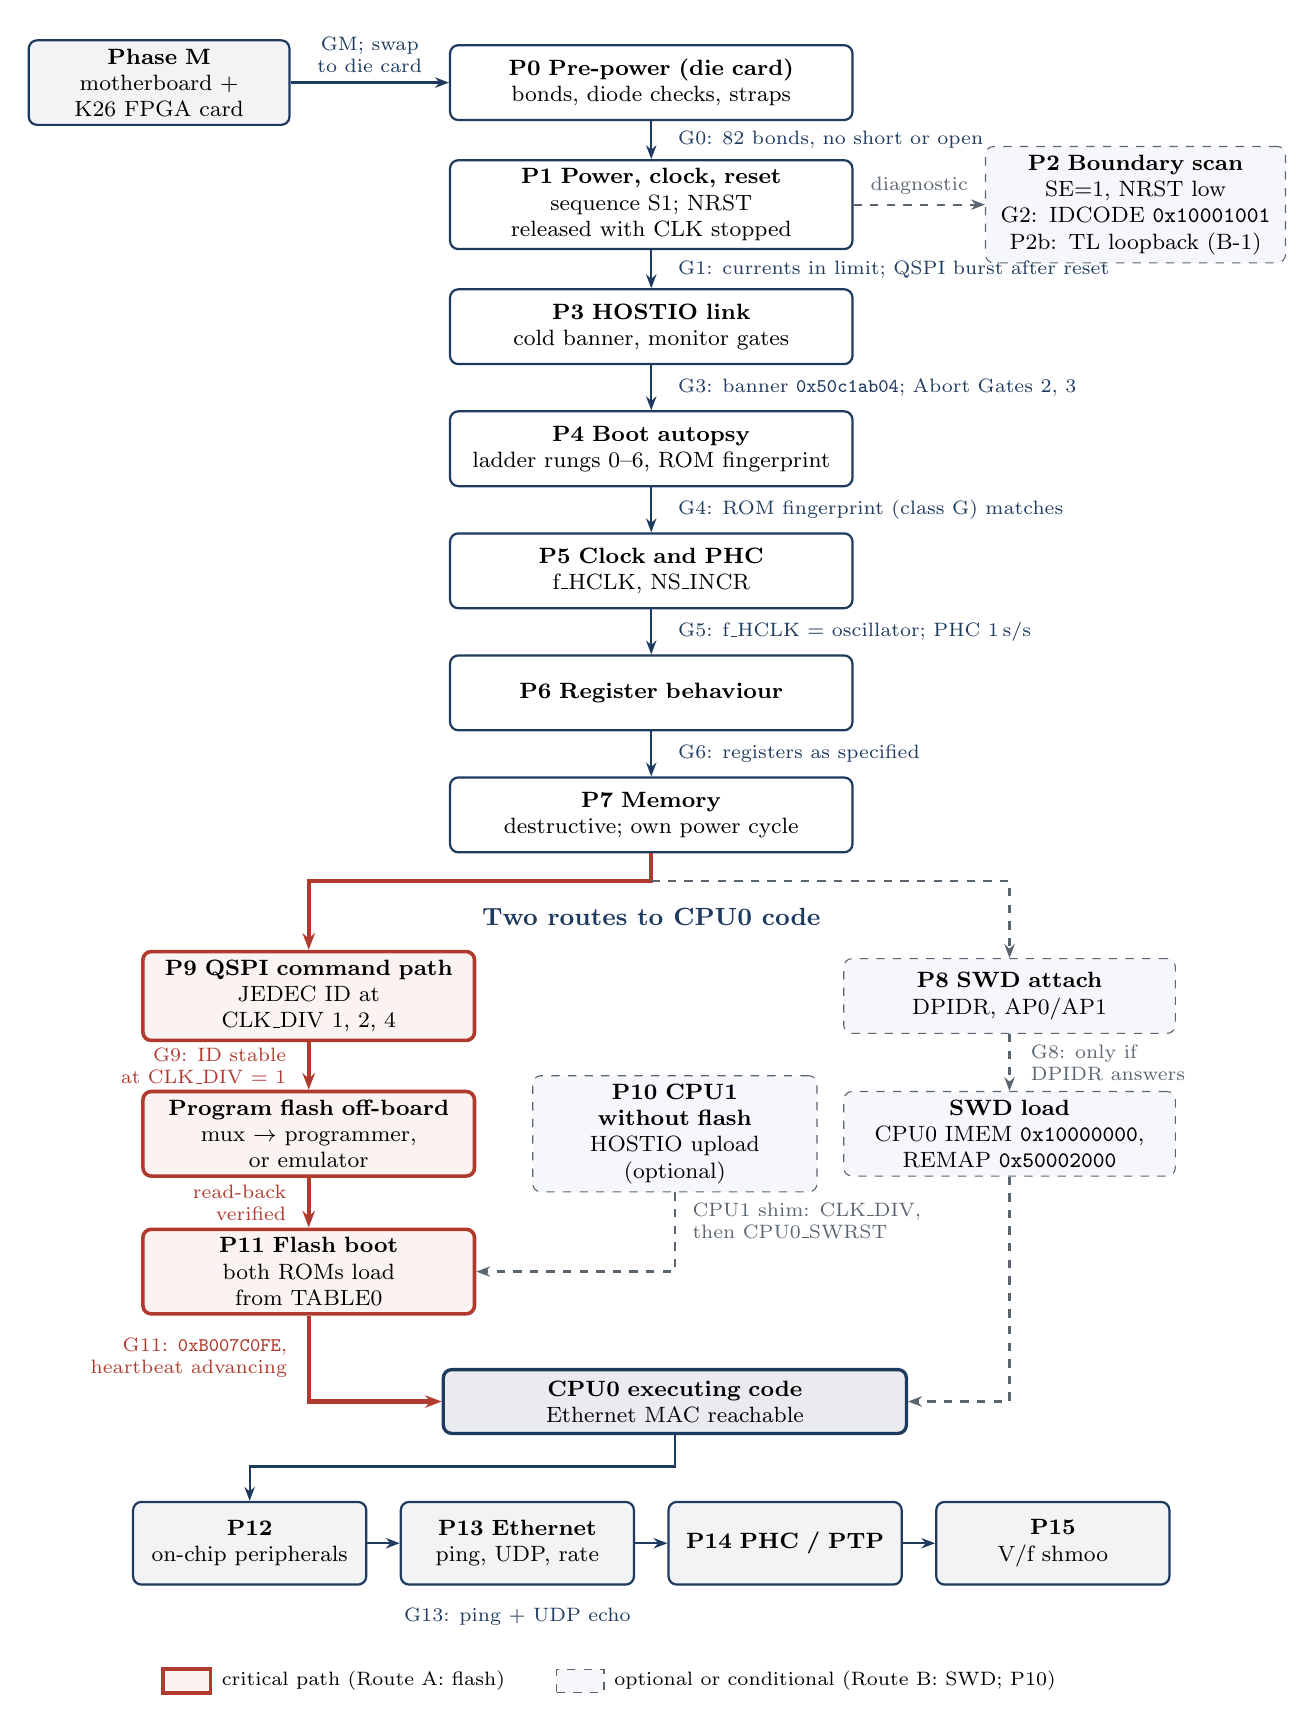
\begin{tikzpicture}[
  font=\footnotesize,
  every node/.append style={execute at begin node=\nohyph},
  ph/.style={draw=accent,thick,rounded corners=3pt,fill=white,align=center,inner sep=3pt,text width=4.9cm,minimum height=0.95cm},
  crit/.style={draw=warn,line width=1.3pt,rounded corners=3pt,fill=warn!6,align=center,inner sep=3pt,text width=4.0cm,minimum height=0.95cm},
  alt/.style={draw=srcgray,dashed,rounded corners=3pt,fill=rowgray,align=center,inner sep=3pt,text width=4.0cm,minimum height=0.95cm},
  fin/.style={draw=accent,thick,rounded corners=3pt,fill=accent!6,align=center,inner sep=3pt,text width=2.75cm,minimum height=1.05cm},
  gate/.style={font=\scriptsize,align=left,text=accent,anchor=west},
  gatel/.style={font=\scriptsize,align=right,text=warn,anchor=east},
  arr/.style={-{Stealth[length=5pt]},thick,draw=accent},
  carr/.style={-{Stealth[length=6pt]},line width=1.6pt,draw=warn},
  darr/.style={-{Stealth[length=5pt]},thick,dashed,draw=srcgray}]
% spine
\node[ph] (p0) at (0,0) {\textbf{P0 Pre-power (die card)}\\ bonds, diode checks, straps};
\node[ph,text width=3.1cm,fill=accent!6] (pm) at (-6.25,0) {\textbf{Phase M}\\ motherboard + K26 FPGA card};
\draw[arr] (pm) -- (p0) node[midway,above,font=\scriptsize,text=accent,align=center] {GM; swap\\ to die card};
\node[ph] (p1) at (0,-1.55) {\textbf{P1 Power, clock, reset}\\ sequence S1; NRST released with CLK stopped};
\node[alt,text width=3.6cm] (p2) at (6.15,-1.55) {\textbf{P2 Boundary scan}\\ SE=1, NRST low\\ G2: IDCODE \texttt{0x10001001}\\ P2b: TL loopback (B-1)};
\node[ph] (p3) at (0,-3.1) {\textbf{P3 HOSTIO link}\\ cold banner, monitor gates};
\node[ph] (p4) at (0,-4.65) {\textbf{P4 Boot autopsy}\\ ladder rungs 0--6, ROM fingerprint};
\node[ph] (p5) at (0,-6.2) {\textbf{P5 Clock and PHC}\\ f\_HCLK, NS\_INCR};
\node[ph] (p6) at (0,-7.75) {\textbf{P6 Register behaviour}};
\node[ph] (p7) at (0,-9.3) {\textbf{P7 Memory}\\ destructive; own power cycle};
\draw[arr] (p0) -- (p1) node[gate,midway,right=6pt] {G0: 82 bonds, no short or open};
\draw[arr] (p1) -- (p3) node[gate,midway,right=6pt] {G1: currents in limit; QSPI burst after reset};
\draw[darr] (p1) -- (p2) node[midway,above,font=\scriptsize,text=srcgray] {diagnostic};
\draw[arr] (p3) -- (p4) node[gate,midway,right=6pt] {G3: banner \texttt{0x50c1ab04}; Abort Gates 2, 3};
\draw[arr] (p4) -- (p5) node[gate,midway,right=6pt] {G4: ROM fingerprint (class G) matches};
\draw[arr] (p5) -- (p6) node[gate,midway,right=6pt] {G5: f\_HCLK = oscillator; PHC 1\,s/s};
\draw[arr] (p6) -- (p7) node[gate,midway,right=6pt] {G6: registers as specified};
% branch
\node[font=\small\bfseries,text=accent] at (0,-10.6) {Two routes to CPU0 code};
\node[crit] (p9) at (-4.35,-11.6) {\textbf{P9 QSPI command path}\\ JEDEC ID at CLK\_DIV 1, 2, 4};
\node[crit] (prog) at (-4.35,-13.35) {\textbf{Program flash off-board}\\ mux $\to$ programmer, or emulator};
\node[crit] (p11) at (-4.35,-15.1) {\textbf{P11 Flash boot}\\ both ROMs load from TABLE0};
\node[alt,text width=3.4cm] (p10) at (0.3,-13.35) {\textbf{P10 CPU1 without flash}\\ HOSTIO upload (optional)};
\node[alt] (p8) at (4.55,-11.6) {\textbf{P8 SWD attach}\\ DPIDR, AP0/AP1};
\node[alt] (swdl) at (4.55,-13.35) {\textbf{SWD load}\\ CPU0 IMEM \texttt{0x10000000}, REMAP \texttt{0x50002000}};
\draw[carr] (p7.south) -- ++(0,-0.35) -| (p9.north);
\draw[darr] (p7.south) ++(0,-0.35) -| (p8.north);
\draw[carr] (p9) -- (prog) node[gatel,midway,left=4pt] {G9: ID stable\\ at CLK\_DIV = 1};
\draw[carr] (prog) -- (p11) node[gatel,midway,left=4pt] {read-back\\ verified};
\draw[darr] (p8) -- (swdl) node[gate,midway,right=4pt,text=srcgray] {G8: only if\\ DPIDR answers};
\draw[darr] (p10.south) -- (0.3,-15.1) -- (p11.east);
\node[font=\scriptsize,text=srcgray,anchor=west,align=left] at (0.4,-14.45) {CPU1 shim: CLK\_DIV,\\ then CPU0\_SWRST};
\node[draw=accent,line width=1.2pt,fill=accent!10,rounded corners=3pt,align=center,text width=5.6cm,inner sep=4pt] (run) at (0.3,-16.75) {\textbf{CPU0 executing code}\\ Ethernet MAC reachable};
\draw[carr] (p11.south) |- (run.west);
\node[gatel,text=warn] at (-4.5,-16.2) {G11: \texttt{0xB007C0FE},\\ heartbeat advancing};
\draw[darr] (swdl.south) |- (run.east);
% final row
\node[fin] (p12) at (-5.1,-18.55) {\textbf{P12}\\ on-chip peripherals};
\node[fin] (p13) at (-1.7,-18.55) {\textbf{P13 Ethernet}\\ ping, UDP, rate};
\node[fin] (p14) at (1.7,-18.55) {\textbf{P14 PHC / PTP}};
\node[fin] (p15) at (5.1,-18.55) {\textbf{P15}\\ V/f shmoo};
\draw[arr] (run.south) -- ++(0,-0.4) -| (p12.north);
\draw[arr] (p12) -- (p13);
\draw[arr] (p13) -- (p14);
\draw[arr] (p14) -- (p15);
\node[gate,anchor=north] at (-1.7,-19.25) {G13: ping + UDP echo};
% legend
\node[draw=warn,line width=1.3pt,fill=warn!6,minimum width=0.6cm,minimum height=0.3cm] (lg1) at (-5.9,-20.3) {};
\node[anchor=west,font=\scriptsize] at (lg1.east) {critical path (Route A: flash)};
\node[draw=srcgray,dashed,fill=rowgray,minimum width=0.6cm,minimum height=0.3cm] (lg2) at (-0.9,-20.3) {};
\node[anchor=west,font=\scriptsize] at (lg2.east) {optional or conditional (Route B: SWD; P10)};
\end{tikzpicture}
\caption[Phase flow]{Phase flow and gates. Phase M proves the motherboard with the K26 FPGA card before the die card goes in. Route A (flash, red) is the plan of record. Route B (SWD) opens only if P8 reads a DPIDR. P10 can load a CPU1 shim that fixes \sig{CLK_DIV} and re-boots CPU0, but CPU0 still loads its code from flash.}
\label{fig:flow}
\end{figure}

\needspace{14\baselineskip}\subsection*{Phase M Motherboard bring-up with the K26 FPGA card}\addcontentsline{toc}{subsection}{Phase M Motherboard bring-up with the K26 FPGA card}
Purpose: prove the motherboard before any die is at risk. Every row below runs with the slot empty or with the \textbf{K26 FPGA card} (CARD\_ID \texttt{001}): a Kria K26I SOM on a slot-format carrier, running the eth-chiplet FPGA build on 3.3\,V LVCMOS IO at CLK = 25\,MHz. The carrier is specified in \sig{FPGA_DAUGHTER_CARD_OPTIONS.pdf}, in this directory. After Phase M the K26 card stays as the \textbf{golden reference}: repeat any later failure on it to separate a motherboard fault from a die fault.

\textbf{Start now, before any board exists: develop the emulator bitstream on the lab KR260s} (same XCK26 family). Undo the QSPI/HOSTIO4 tie-offs, take CLK from a pin, build with the silicon \sig{stage0_bootrom}/\sig{stage0_bootrom_chip_core} ROMs, and target the \texttt{-i} part (\sig{xck26-sfvc784-2LV-i}). Start from the HAPS-SX board top, which already wires QSPI, HOSTIO, SWD and RMII and uses the silicon ROM. The KR260 + paddle adapter to the slot is \textbf{optional}: build it only if the motherboard is ready well before the K26 card.
\phasebegin\begin{tabularx}{\textwidth}{@{}P{0.75cm}LP{4.7cm}C{0.95cm}P{3.3cm}C{1.05cm}@{}}\phasehead
M.1 & Slot empty: host MCU reads the card-detect pins & CARD\_ID = \texttt{111}, both \sig{CARD_PRESENT_n} high; the script refuses every rail & B & board-control script & \NW \\
M.2 & Rails at the slot pins (engineering override, slot empty or electronic load): VDD\_CORE sweep 1.00--1.25\,V into the DNP dummy load; VDDIO 3.3\,V; VIN\_AUX 5\,V at 4\,A & Each within tolerance at the slot; INA228 agrees with a DMM; a setpoint above 1.25\,V is refused; current limits and the VIN\_AUX eFuse trip as set & B & board-control script; INA228 & \NW \\
M.3 & Clocks at the slot: CLK at 25, 50 and 100\,MHz; OE off and on; REF\_CLK at the PHY and the slot & Frequency and edges ($\le$ 1.2\,ns) correct; clean restart after OE, no runt pulse; CLK rests low while disabled & B & scope at \sig{TP_CLK}, \sig{TP_REFCLK} & \PR \\
M.4 & Insert the K26 card (mechanical support fitted) with all rails off; power it & CARD\_ID = \texttt{001}, both PRESENT low. VDDIO and VIN\_AUX on; VDD\_CORE reads 0\,V. Slot pull levels unchanged until CARD\_READY is released (bus switches open: IOACK high, QSPI\_IO1 low). The host waits for CARD\_READY & B & board-control script & \NW \\
M.5 & HOSTIO link through the header and the slot to the FPGA build & HIO-001 banner; Tier 0 passes against the FPGA target's reference values (25\,MHz) & H & RP2350 + \sig{hostio_suite} (FPGA target) & \EX \\
M.5a & Card JTAG through the slot's spare pins & The motherboard's card-JTAG header sees the K26 chain & J & J-Link / Vivado HW server & \NW \\
\bottomrule\end{tabularx}\phaseend
\phasebegin\begin{tabularx}{\textwidth}{@{}P{0.75cm}LP{4.7cm}C{0.95cm}P{3.3cm}C{1.05cm}@{}}\phasehead
M.6 & Scripted sequence S1 (NRST, CLK\_OE, rail enables) & On the scope: NRST rises while CLK is stopped, CLK starts after the supervisor timeout; the FPGA build reacts if it takes NRST/CLK from the slot & B+H & board-control script & \NW \\
M.7 & Flash path: mux to side B, program IMG-1, verify; mux to side A; read JEDEC ID and TABLE0 magic from the slot side & Programmer read-back identical. Through the slot: ID matches the part, magic \texttt{0x424F4F54} & P+H & programmer flow; P9 script & \NW \\
M.8 & PHY: link to the host PC; MDIO scan from the FPGA build & Link up at 100\,Mb/s; PHY ID \texttt{0x0007/0xC0F1}, stable (MDIO pull-up correct) & F+host & FPGA build firmware & \PA \\
M.9 & SWD and JTAG headers: continuity to the slot pins in each isolation-link set (rails off, card out) & Matches Table~\ref{tab:links} & B & DMM & \PR \\
M.10 & Force one \sig{CARD_PRESENT_n} high at \sig{TP_PRESENT} while powered (do not pull the card) & The host drops every slot rail at once & B & board-control script & \NW \\
\bottomrule\end{tabularx}\phaseend
\begin{gatebox}\textbf{Gate GM.} Rails, clamp, eFuse and card-detect/CARD\_READY gating, all three clocks and OE, the HOSTIO link, card JTAG, the flash path through the slot, the PHY link and the scripted S1 all work on the K26 card. Then power everything down, remove the K26 card, and insert the die card for P0.\end{gatebox}

\needspace{14\baselineskip}\subsection*{P0 Pre-power (die card bonded, not powered)}\addcontentsline{toc}{subsection}{P0 Pre-power (die card bonded, not powered)}
Purpose: find shorts, opens and wrong straps before any current flows. Rows 0.2--0.6 run on the die card \emph{out of the slot}, measured at its edge fingers, so only the card's own parts load the readings. ERC and PadShorts were never run on rc4, and LVS is blind at the pad boundary \src{REG:464-477,497-499}.
\phasebegin\begin{tabularx}{\textwidth}{@{}P{0.75cm}LP{4.7cm}C{0.95cm}P{3.3cm}C{1.05cm}@{}}\phasehead
0.1 & Host stack dry run: status-nibble fix, resync watchdog, capture to file & Verified in Phase M against the FPGA card & B & \src{PROC:247-280} & \EX \\
0.2 & Bare-card signature \emph{before bonding}: DMM resistance and diode reading from every card-edge finger & Matches the card schematic (pull values; no finger-to-finger short) & B & this plan & \PR \\
0.3 & Bond inspection and photographs & 82 wires, no crossings, no wire near the die edge & B & bonder & \PR \\
0.4 & Diode check of every signal finger to VSSIO and to VDDIO, compared with 0.2 & Every signal pad adds the die's ESD-diode signature; no short, no missing diode (an open bond); consistent across boards & B & \src{REG:473-477} & \PR \\
0.5 & Rail-to-rail resistance at the card fingers: VDD--VSS, VDDIO--VSSIO, VDD--VDDIO & No short; values recorded & B & -- & \PR \\
0.6 & Strap and population check & Card: TEST low, SE pull-down, TL\_RX pulls fitted, loopback links not fitted, CARD\_ID straps \texttt{000}. Motherboard: SE jumper off, mux on side A, links in the HOSTIO set (Table~\ref{tab:links}) & B & Section~\ref{sec:partition} & \PR \\
0.7 & Insert the die card with every rail off & Both \sig{CARD_PRESENT_n} low; CARD\_ID reads \texttt{000} & B & board-control script & \NW \\
\bottomrule\end{tabularx}\phaseend
\begin{gatebox}\textbf{Gate G0.} All rows pass. On any short or open: stop, photograph, and re-inspect the bonds before applying power. Apply the glob top only after G0 passes (a bond can still be lifted to isolate a pad before then).\end{gatebox}

\needspace{14\baselineskip}\subsection*{P1 Power, clock and reset}\addcontentsline{toc}{subsection}{P1 Power, clock and reset}
Purpose: bring up the rails with current limits and start the die with the N1-safe sequence S1 (Section~\ref{sec:power}).
\phasebegin\begin{tabularx}{\textwidth}{@{}P{0.75cm}LP{4.7cm}C{0.95cm}P{3.3cm}C{1.05cm}@{}}\phasehead
1.0 & S1 step 0: card check & Rails are enabled only after CARD\_ID = \texttt{000} and both PRESENT low & B & board-control script & \NW \\
1.1 & VDDIO only (VDD off), limit 50\,mA & Stable; no current limit hit. Record it (no reference value exists) & B & INA228 & \PR \\
1.2 & VDD ramp to 1.20\,V in 0.1\,V steps, CLK stopped, NRST low, limit 100\,mA; read the voltage at the card (Kelvin sense) & Monotonic, near leakage. Stop above about 10\,mA static (start value) & B & INA228; \src{REG:403-405} & \PR \\
1.3 & Thermal check & No hot spot on the die or the regulators & B & thermal camera & \PR \\
1.4 & CLK on (50\,MHz) with NRST still low & \sig{TP_CLK} frequency and swing correct, edges $\le$ 1.2\,ns; record \sig{VDD_DIE} in reset & B & scope; \src{SDC:66-67} & \PR \\
1.5 & S1 steps 6--7: stop CLK, release NRST, start CLK & \sig{VDD_DIE} current rises and settles below 50.7\,mA. A QSPI\_nCS and SCLK burst at CLK/2 appears within milliseconds: CPU1's ROM is running & B & scope on \sig{TP_QSPI_x}; \src{REG:170-176,227-252} & \PR \\
\bottomrule\end{tabularx}\phaseend
\begin{gatebox}\textbf{Gate G1.} Currents are within limits, CLK is clean, and a QSPI burst follows reset release. If there is no QSPI activity, CPU1's ROM is not running: check CLK, NRST, SE and TEST with the scope before touching HOSTIO.\end{gatebox}

\needspace{14\baselineskip}\subsection*{P2 Boundary scan (own session; diagnostic)}\addcontentsline{toc}{subsection}{P2 Boundary scan (own session; diagnostic)}
Session setup: NRST low; HOSTIO host unplugged; boundary-scan links fitted (Table~\ref{tab:links}); SE raised \emph{before} TDI is driven; TCK about 1\,MHz. Every net on HOSTIO4\_P1[6:2], QSPI\_IO[3:0] and RMII\_MDIO high-Z on the board side (the walk drives them). Ready-made SVFs, generated from the BSDL and replayed clean against the RTL; the rc4 netlist passes the gate bench 7/7: \sig{p2_idcode.svf}, \sig{p2_bypass.svf}, \sig{p2_sample.svf}, \sig{p2_extest_walk.svf}, \sig{p2_extest_walk_tlloop.svf} (in \sig{build/presilicon-closure/item14/svf/}; \src{docs/chip-reference-manual/review/closure/item14-bscan.md}). \sig{PIN_MAP} in the BSDL still needs the card nets (B-7). Boundary scan works with the core dead, so run it early if P3 fails.
\phasebegin\begin{tabularx}{\textwidth}{@{}P{0.75cm}LP{4.7cm}C{0.95cm}P{3.3cm}C{1.05cm}@{}}\phasehead
2.1 & IDCODE, 64-bit shift & \texttt{0x10001001}, IR length 4 & J & \src{BSC:201-231} & \NW{} script \\
2.2 & BYPASS (\texttt{1111}); boundary-register length & Exactly 1 stage; 76 cells & J & \src{BSC:254-271} & \NW \\
2.3 & SAMPLE, then PRELOAD and EXTEST: drive pattern P and its inverse, then walk a 1 through every driven cell & Outputs toggle as loaded, seen at the test points. Input cells capture board levels; they are observe-only & J & BSDL \src{sys_desc/bscan/*.bsdl}; \src{BSC:332-412} & \NW \\
2.4 & With the B-1 loopback fitted: \sig{p2_extest_walk_tlloop.svf} & All nine lanes continuous, clock mid-bus in ring order & J & \src{BSC:450-476} & \NW \\
\bottomrule\end{tabularx}\phaseend
\begin{gatebox}\textbf{Gate G2 (diagnostic).} IDCODE reads correctly: the pad ring and the TAP are alive. A failure here does not block P3, but record it. At session end: SE low, links back to the HOSTIO set. HIGHZ is not implemented and CLAMP is untested.\end{gatebox}

\needspace{14\baselineskip}\subsection*{P2b TL loopback (new, B-1; loopback footprints fitted; diagnostic)}\addcontentsline{toc}{subsection}{P2b TL loopback (new, B-1)}
Runs after P3 has a working HOSTIO link and P2's 2.4 has shown the nine lanes continuous. One die is both ends of its own link: its TL\_CLK\_TX is its RX clock. Bring it up at the lowest link clock (CLK = 50\,MHz) and scope \sig{TL_CLK_RX} at the die first: one lost link-clock edge is enough to wedge the link \src{docs/chip-reference-manual/review/closure/item07-d2d-traffic.md}.
\phasebegin\begin{tabularx}{\textwidth}{@{}P{0.75cm}LP{4.7cm}C{0.95cm}P{3.3cm}C{1.05cm}@{}}\phasehead
2b.1 & Fit the 0\,\textohm{} links; power cycle; S1 & P1--P3 results unchanged & B & -- & \PR \\
2b.2 & Write ROLE\_CFG \texttt{0x2E032080} = \texttt{0x02} (die\_a) or \texttt{0x03} (die\_b) over HOSTIO; poll link status \texttt{0x2E032084} & cal\_done and all 7 FC nodes at state 4; in rc4-RTL sim at 23.7\,ms at 50\,MHz, with no further host steps & H & \src{docs/chip-reference-manual/review/closure/item03-d2d-loopback.md} & \NW \\
2b.3 & Program the CAM (\texttt{0x2F}$\to$\texttt{0x2D}); write 16 words through \texttt{0x2F001000} (word, halfword, byte), read back through \texttt{0x2D} and \texttt{0x2F} with the M0+ or HOSTIO, never the DMA-250 & Byte-exact, no bus error, CRC error counters 0 & H/F & \src{docs/chip-reference-manual/review/closure/item03-d2d-loopback.md} & \NW \\
2b.4 & If \sig{tl_data_mode} stalls or a lane shows a persistent sync error just after training: re-arm training and count retries & At most one retrain (CDC class D: calibrator$\to$TX single-flop; R1 reset release) & H & \src{docs/chip-reference-manual/review/closure/item12-cdc.md} \S4 & \NW \\
\bottomrule\end{tabularx}\phaseend
\begin{gatebox}\textbf{Gate G2b (diagnostic).} The die trains against itself and moves data byte-exact: the shipped D2D configuration works through real pads at real CLK. A peer bus error or timeout means POR (power cycle) and retry, never a one-sided retry. A failure does not block P3--P15; remove the links afterwards if they load the TX pads.\end{gatebox}

\needspace{14\baselineskip}\subsection*{P3 HOSTIO link}\addcontentsline{toc}{subsection}{P3 HOSTIO link}
\phasebegin\begin{tabularx}{\textwidth}{@{}P{0.75cm}LP{4.7cm}C{0.95cm}P{3.3cm}C{1.05cm}@{}}\phasehead
3.1 & HIO-001 cold banner (capture $\ge$ 10\,s from S1 step 5) & Exactly one \texttt{0x50c1ab04} within 1\,s. \texttt{0x50c1ab01} = wrong (ADPBASIC) build. Several banners = die resetting & H & \src{PROC:298-320}; T0 & \EX \\
3.2 & HIO-002/003/004/010: monitor entry, bad-command rejection, exit and re-entry & Abort Gate 2 passes & H & \src{PROC:340-346}; T0 & \EX \\
3.3 & HIO-005/006/008/009/011/120: address register, size encoder, auto-increment, block dump & All pass. If HIO-006 fails, every later access has the wrong size: stop & H & T0 & \EX \\
3.4 & HIO-007 \sig{R!} control pair & \texttt{0x30000000} returns \sig{R!}; \texttt{0x08000000} returns \texttt{0x18003c00} & H & \src{PROC:346}; T0 & \EX \\
\bottomrule\end{tabularx}\phaseend
\begin{gatebox}\textbf{Gate G3.} Banner plus Abort Gates 2 and 3. \textbf{No banner (Abort Gate 1)} does \emph{not} mean a dead die. Six of the fourteen causes in PROC \S1.6 give this symptom: wrong pin map, floating CLK or NRST, SE high, the wrong host driver polarity, among others. Scope \sig{TP_IOACK} and \sig{TP_IOREQ1} and work PROC \S9.1 before concluding anything about silicon.\end{gatebox}

\needspace{14\baselineskip}\subsection*{P4 Boot autopsy and identity}\addcontentsline{toc}{subsection}{P4 Boot autopsy and identity}\label{sec:p4}
Read the ladder before anything else and record every rung. With blank flash (IMG-0) and the QSPI\_IO1 pull-down, expect all rungs present and rung 6 = \texttt{0x4}. The HardFault diagnosis in PROC \S0.3 is superseded by \src{REG:227-253}: a missing flash does not fault CPU1.
\phasebegin\begin{tabularx}{\textwidth}{@{}P{0.75cm}LP{4.7cm}C{0.95cm}P{3.3cm}C{1.05cm}@{}}\phasehead
4.1 & HIO-106 ladder: rung 0 \texttt{0x800000E4}; 1 \texttt{0x98000200}; 2 \texttt{0x21000030}; 3 \texttt{0x21000000}[8]; 4 \texttt{0x23000010}; 5 \texttt{0x98000084}; 6 \texttt{0x29000000} & \texttt{0x08000678}; \texttt{0x0F1C0DE1}; \texttt{0x0000800B}; 1; \texttt{0xD15C0001}; \texttt{0xFFFFFFFF} (blank) or table data; \texttt{0x4} (no image) or \texttt{0x5} (CPU1 app). If rung 6 reads 0, re-read after 60\,s & H & \src{PROC:86-97}; T1 & \EX \\
4.2 & HIO-101/102 ROM fingerprint (class G, mask-verified) & e.g.\ eth ROM +0x0E4 = \texttt{0x0800048c}; cc ROM +0x0E4 = \texttt{0x08000678} (full list PROC \S8.4) & H & \src{PROC:995-1015}; T1 & \EX \\
4.3 & HIO-103--127 identity; HIO-114 census & As PROC; eth DMEM word 0 reads \texttt{0x00000000} on the ASIC (not the FPGA value) & H & \src{PROC:125}; T1 & \EX \\
4.4 & One-shot$\ast$: read uninitialised SRAM on the first power-up & Record; decides whether HIO-107's replacement works & H & \src{PROC:1172} & \PR \\
\bottomrule\end{tabularx}\phaseend
\begin{gatebox}\textbf{Gate G4.} The ROM fingerprint matches; a class-G mismatch is a hard finding. The ladder is classified. If rung 4 is published and rung 6 still reads 0 on a re-read, that is the only silicon finding in the ladder.\end{gatebox}

\needspace{14\baselineskip}\subsection*{P5 Clock and PHC}\addcontentsline{toc}{subsection}{P5 Clock and PHC}
\phasebegin\begin{tabularx}{\textwidth}{@{}P{0.75cm}LP{4.7cm}C{0.95cm}P{3.3cm}C{1.05cm}@{}}\phasehead
5.1 & HIO-402: f\_HCLK from the perf probe over a host-timed interval $\ge$ 15\,s & Matches the oscillator within its tolerance & H & \src{PROC:447-467}; T45 & \EX \\
5.2 & Write \sig{NS_INCR} = $10^9/f$ to \texttt{0x22000008} (20 at 50\,MHz); HIO-403/404 & PHC advances $10^9$\,ns per second within oscillator tolerance. Reset value 4 runs time at 0.2$\times$ at 50\,MHz & H & \src{PROC:595-619}; \src{REG:341}; T45 & \EX \\
5.3 & HIO-311/406: CPU1 timers & Count down & H & T23/T45 & \EX \\
\bottomrule\end{tabularx}\phaseend
\begin{gatebox}\textbf{Gate G5.} The measured clock equals the oscillator, and PHC time runs at 1\,s/s. Derive every later timing figure from the measured f, not the nominal one.\end{gatebox}

\needspace{14\baselineskip}\subsection*{P6 Register behaviour}\addcontentsline{toc}{subsection}{P6 Register behaviour}
\phasebegin\begin{tabularx}{\textwidth}{@{}P{0.75cm}LP{4.7cm}C{0.95cm}P{3.3cm}C{1.05cm}@{}}\phasehead
6.1 & HIO-301--314. Gate 8 is HIO-313, with its control at \texttt{0x2100000C} & As specified & H & \src{PROC:536-585}; T23 & \EX \\
6.2 & HIO-305 mailbox; HIO-304 spinlock (DBG page \texttt{0x2C100200} only) & As specified; no lock left held & H & \src{PROC:591}; T23 & \EX \\
6.3 & HIO-411 DMA-250 ID at \texttt{0x20000FC8} & \texttt{0x2500043B}: present and not power-gated & H & \src{PROC:1034}; T45 & \EX \\
\bottomrule\end{tabularx}\phaseend
\begin{gatebox}\textbf{Gate G6.} All pass. A B-class row that goes red is a documentation finding until the RTL proves otherwise \src{PROC:1126}.\end{gatebox}

\needspace{14\baselineskip}\subsection*{P7 Memory (destructive; separate power cycle)}\addcontentsline{toc}{subsection}{P7 Memory (destructive; separate power cycle)}
Tier-2 tests wipe eth IMEM and shared SRAM. Run them in their own power cycle, and never before a firmware-dependent test in the same power cycle \src{PROC:1147}.
\phasebegin\begin{tabularx}{\textwidth}{@{}P{0.75cm}LP{4.7cm}C{0.95cm}P{3.3cm}C{1.05cm}@{}}\phasehead
7.1 & HIO-118, HIO-201--211 on all five RAMs: eth IMEM 32\,KB, eth DMEM 16\,KB, CPU1 IMEM 16\,KB, CPU1 DMEM 8\,KB, shared SRAM 8\,KB & Walking 1s and 0s, address-in-address and fill all pass. About 1.5\,h with full dumps & H & \src{PLAN:496-506}; T23 & \EX \\
7.2 & At-speed March test in firmware & No failures (there is no MBIST) & F & -- & \NW \\
\bottomrule\end{tabularx}\phaseend
\begin{gatebox}\textbf{Gate G7.} No memory faults. Power-cycle before P8 onwards.\end{gatebox}

\needspace{14\baselineskip}\subsection*{P8 SWD attach (Route B; not on the critical path)}\addcontentsline{toc}{subsection}{P8 SWD attach (Route B; not on the critical path)}
\phasebegin\begin{tabularx}{\textwidth}{@{}P{0.75cm}LP{4.7cm}C{0.95cm}P{3.3cm}C{1.05cm}@{}}\phasehead
8.1 & J-Link BASE, JTAG-to-SWD switch sequence, read DPIDR. Keep SE = 0. Leave HOSTIO idle (two-master rule) & A DPIDR is read. The expected value is \NF: record what comes back & S & \src{NMS/docs/SWD_REFLASH_ASIC.md}; \src{REG:215-216} & \NW{} config \\
8.2 & AP0 (CPU0, \texttt{0xA0000000}) and AP1 (CPU1, \texttt{0xB0000000}) by hand (no ROM table); single accesses with read-back & Halt and resume both cores; read the MAC MODER at \texttt{0x40000000} & S & \src{REG:313-319,342} & \NW \\
8.3 & If 8.1 passes: halt CPU0, load an image at \texttt{0x10000000}, set REMAP \texttt{0x50002000} = 1, resume & CPU0 image signature appears & S & \src{NMS/docs/SWD_REFLASH_ASIC.md:289-328} & \PA \\
\bottomrule\end{tabularx}\phaseend
\begin{gatebox}\textbf{Gate G8.} A DPIDR is read: Route B is open. Otherwise record the result and continue on Route A. SWD failing is not a blocker.\end{gatebox}

\needspace{14\baselineskip}\subsection*{P9 QSPI command path}\addcontentsline{toc}{subsection}{P9 QSPI command path}
Run at \textbf{CLK = 50\,MHz}: STA predicts $+5.0$\,ns read margin at SS with CLK\_DIV = 1, and a fail at 100\,MHz \src{docs/chip-reference-manual/review/closure/item06-sta.md} \S6c. Use the APB command path only; \textbf{never touch \texttt{0x24xxxxxx}} (HZ-6). Program the flash off-board through the mux, never from HOSTIO on the first die \src{PROC:1143}.
\phasebegin\begin{tabularx}{\textwidth}{@{}P{0.75cm}LP{4.7cm}C{0.95cm}P{3.3cm}C{1.05cm}@{}}\phasehead
9.1 & Read the JEDEC ID through \texttt{0x21000008}/\texttt{0x21000010} at CLK\_DIV = 1, 2, 4 & ID matches the fitted part at every divider. The two in-tree FPGA notes on the command format disagree & H & \src{REG:276-279}; HIO-312/115 & \NW{} script \\
9.2 & After off-board programming, read the TABLE0 magic at flash \texttt{0x000000} through the same path & \texttt{0x424F4F54} ("BOOT") & H & \src{AMAP:393} & \NW \\
\bottomrule\end{tabularx}\phaseend
\begin{gatebox}\textbf{Gate G9.} Reads are consistent at CLK\_DIV = 1, the ROM's rate (SCLK = CLK/2). If only CLK\_DIV $\ge$ 2 works at 50\,MHz, the ROM boot will fail and the fault is the board or flash, not the predicted die limit. Lower CLK, or use REG \S3.1 workaround 2 (write CLK\_DIV, then pulse CPU0\_SWRST) or 3 (the CPU1 shim).\end{gatebox}

\needspace{14\baselineskip}\subsection*{P10 CPU1 without flash (optional; sim-proven, never run on a die)}\addcontentsline{toc}{subsection}{P10 CPU1 without flash (optional; sim-proven, never run on a die)}
Two hazards: setting \texttt{0x29000000} bit 0 is irreversible until power-on (HZ-4), and \sig{CPU1_SWRST} drops the HOSTIO link (HZ-5). The docs disagreed on whether this route exists (\src{REG:258} and \src{PROC:850-873} say yes; \src{HFW:319} says no). The rc4-RTL dry run settles it: \textbf{the route works} (CPU1 runs the uploaded image) \src{docs/chip-reference-manual/review/closure/item08-bringup-dryrun.md}. But the repo's \sig{fw_cpu1_park.bin} writes no signature, so 10.2 cannot pass until \sig{fw_cpu1_park.S} writes \texttt{0x48465701} to \texttt{0x2D000008}.
\phasebegin\begin{tabularx}{\textwidth}{@{}P{0.75cm}LP{4.7cm}C{0.95cm}P{3.3cm}C{1.05cm}@{}}\phasehead
10.1 & Four-command write/read-back at \texttt{0x90003ff0} & Value sticks & H & \src{PROC:866-873} & \EX \\
10.2 & Upload image to \texttt{0x90000000}; set \texttt{0x29000000} bit 0; \texttt{0x2A000020} = 2; re-enter the link & Park-image signature \texttt{0x48465701} at \texttt{0x2D000008} & H & \src{PROC:683-742}; the suite refuses HIO-508 \src{tier4_5.py:850} & \NW{} shim \\
\bottomrule\end{tabularx}\phaseend
\begin{gatebox}\textbf{Gate G10.} CPU1 runs uploaded code. That opens the CPU1-shim route: set CLK\_DIV, AHB\_SETUP and XIP\_ACTIVE, publish \texttt{0xD15C0001}, then pulse CPU0\_SWRST. CPU0 still needs a valid flash image.\end{gatebox}

\needspace{14\baselineskip}\subsection*{P11 Flash boot (critical path)}\addcontentsline{toc}{subsection}{P11 Flash boot (critical path)}
Run at \textbf{CLK = 50\,MHz}. Raise CLK only after P11 passes and firmware has set CLK\_DIV $\ge$ 2: at CLK\_DIV = 1 the read fails above $\approx$66\,MHz at SS. Check the image with \sig{check_flash.py} before programming (flash-layout rule, Section~\ref{sec:images}).
\phasebegin\begin{tabularx}{\textwidth}{@{}P{0.75cm}LP{4.7cm}C{0.95cm}P{3.3cm}C{1.05cm}@{}}\phasehead
11.1 & Program IMG-1 off-board (mux on side B), verify by read-back, set the mux to side A & Read-back identical; sha256 logged & P & -- & \NW{} flow \\
11.2 & Power-cycle with S1; read the ladder & Rung 6 = \texttt{0x5}: CPU1 is running its app & H & \src{PROC:86-97} & \EX \\
11.3 & Read the CPU0 signatures & \texttt{0x2D001FF0} = \texttt{0xB007C0FE}; \texttt{0x2D000004} = \texttt{0x5E27C0DE}; \texttt{0x2D000008} = \texttt{0x48465702}; \texttt{0x2D00000C} = \sig{FW_CORE_HZ}; \texttt{0x2D000000} advancing & H & \src{HFW:74-94,426-436} & \EX \\
11.4 & Five further power cycles & Boots 5/5. The primary table is retried last after the counter trips & H & \src{ROM1:344-362} & \PR \\
\bottomrule\end{tabularx}\phaseend
\begin{gatebox}\textbf{Gate G11.} CPU0 runs code from flash, so the MAC is now reachable: the critical path is closed. If P9 passed but P11 fails, run \sig{check_flash.py} on the programmed bytes, then check entry order and the \sig{FW_CORE_HZ} build.\end{gatebox}

\needspace{14\baselineskip}\subsection*{P12 On-chip peripherals via firmware}\addcontentsline{toc}{subsection}{P12 On-chip peripherals via firmware}
Results go to DMEM through \sig{regr_sentinel.h}, read over HOSTIO at \texttt{0x18000000}. Apps live in \sig{NMS/firmware/apps/}; each needs an ASIC build packed into a flash image.
\phasebegin\begin{tabularx}{\textwidth}{@{}P{0.75cm}LP{4.7cm}C{0.95cm}P{3.3cm}C{1.05cm}@{}}\phasehead
12.1 & NVIC, peripheral IRQs, CPU0 timer and watchdog & Sentinel pass & F & \sig{network_core_nvic_selftest}, \sig{network_core_periph_irq_delivery} & \PA \\
12.2 & CPU1 watchdog reset and RESET\_INFO & Reset cause recorded (HIO-302) & F+H & \sig{chip_core_wdog_reset} & \PA \\
12.3 & IPC doorbell both ways; spinlock hammer & Doorbell fires once; no lost updates & F & \sig{ipc_irq_*}, \sig{ring_2core_hammer_*} & \PA \\
12.4 & DMA-250 copy \textbf{within one port only}, verified by read-back & Data correct; DONE alone is not proof (HSEL erratum) & F/H & \sig{dma250_done_semantics} & \PA \\
12.5 & CRC accelerator & Matches the software CRC & F & \sig{crc_accel_selftest} & \PA \\
\bottomrule\end{tabularx}\phaseend
\begin{gatebox}\textbf{Gate G12.} Every row passes or is logged against a known erratum (Section~\ref{sec:errata}).\end{gatebox}

\needspace{14\baselineskip}\subsection*{P13 Ethernet}\addcontentsline{toc}{subsection}{P13 Ethernet}
Needs the 50\,MHz REF\_CLK and the PHY. Rebuild the apps for the board CLK: the MDIO divider is hard-coded for 25\,MHz.
\phasebegin\begin{tabularx}{\textwidth}{@{}P{0.75cm}LP{4.7cm}C{0.95cm}P{3.3cm}C{1.05cm}@{}}\phasehead
13.1 & MAC reset values (IMG-2) & MODER = \texttt{0x0000A000}, PACKETLEN = \texttt{0x00400600} & F & \sig{hostio_fw/fw_mdio_probe.c}; \src{PROC:879} & \EX \\
13.2 & MDIO scan & Stable PHY ID \texttt{0x0007/0xC0F1} at the strapped address; zero BUSY time-outs & F & same; \src{HFW:78-93} & \EX \\
13.3 & MAC internal loopback & Frame returns byte-exact & F & \sig{eth_mac_loopback} & \PA \\
13.4 & PHY loopback; link and autonegotiation & Frames seen; link up at 100\,Mb/s & F & \sig{eth_tsu_watermark}, \sig{eth_phy_link} & \PA \\
13.5 & ARP and ICMP ping from the host & Replies; 0\,\% loss over 1000 pings & F+host & \sig{eth_ping_responder} (192.168.10.2) & \PA \\
13.6 & UDP echo, port 7 & Echo returns byte-exact & F+host & \sig{eth_netapp} (PicoTCP) & \PA \\
13.7 & Throughput & Rate measured and recorded & host & Scapy scenarios exist & \NW \\
\bottomrule\end{tabularx}\phaseend
\begin{gatebox}\textbf{Gate G13.} Ping and UDP echo work: this is the board's main deliverable. Do not toggle LOOPBCK or TXEN mid-traffic (no CDC sign-off, REG N5); poll rather than rely on the TX-complete IRQ.\end{gatebox}

\needspace{14\baselineskip}\subsection*{P14 PHC and PTP}\addcontentsline{toc}{subsection}{P14 PHC and PTP}
\phasebegin\begin{tabularx}{\textwidth}{@{}P{0.75cm}LP{4.7cm}C{0.95cm}P{3.3cm}C{1.05cm}@{}}\phasehead
14.1 & PHC register and alarm coverage; signed FRAC trim & Pass; rate within the ppm target & F/H & \sig{phc_selftest}, \sig{phc_reg_coverage}, \sig{phc_alarm_irq_pulse} & \PA \\
14.2 & PTP slave against a host grandmaster & Offset converges & F+host & \sig{ptp_slave}: hard-codes \sig{NS_INCR} = 40 and reports over a UART with no pad, so port it first & \PA \\
\bottomrule\end{tabularx}\phaseend
PPS output cannot be tested: it has no pad.

\needspace{3\baselineskip}\subsection*{P15 Characterisation}\addcontentsline{toc}{subsection}{P15 Characterisation}
See Section~\ref{sec:char}.

\needspace{12\baselineskip}
% =====================================================================
\section{Firmware, applications and host tools to build}\label{sec:fw}
% =====================================================================
Efforts are engineer-days, from research report 02 unless marked \textsuperscript{p} (this plan's estimate). ``Needed by'' is the first phase that cannot run without the item.

{\footnotesize
\setlength{\tabcolsep}{4pt}
\begin{longtable}{@{}P{0.45cm}P{4.4cm}P{1.3cm}P{5.2cm}P{1.5cm}P{2.4cm}@{}}
\toprule
\rowcolor{headgray}[0pt][0pt]\hd{\#} & \hd{Item} & \hd{Status} & \hd{Path} & \hd{Effort (d)} & \hd{Needed by}\\
\midrule
\endfirsthead
\toprule
\rowcolor{headgray}[0pt][0pt]\hd{\#} & \hd{Item} & \hd{Status} & \hd{Path} & \hd{Effort (d)} & \hd{Needed by}\\
\midrule
\endhead
\multicolumn{6}{@{}l}{\cellcolor{rowgray}\textbf{Tier A: before first power}}\\
0 & K26 FPGA card (slot carrier) and the emulator bitstream for the \texttt{-i} part, developed on the lab KR260s now & separate study & \sig{FPGA_DAUGHTER_CARD_OPTIONS.pdf} (this directory) & see study & Phase M \\
1 & HOSTIO host adapter re-verify (RP2350 PIO driver) & \EX & \src{NMS/nanosoc_arch_tech/rtl/hostio4/rpi-pico-pio/pico-mp/hostio-pio.py} & 0.5 & P0 \\
2 & HOSTIO client and suite, ASIC target; place \sig{golden_asic_reference.json} (generated by closure item 8) & \PA & \src{RIG/hostio_adp.py}, \src{RIG/hostio_suite} & 1 & P3 \\
3 & Board-control library: CARD\_ID/PRESENT/READY gating, VIN\_AUX eFuse, sequence S1, INA228 logging, TPS62869 clamp, CLK\_OE, NRST, mux, PHY reset & \NW & -- & 1--2\textsuperscript{p} & Phase M \\
4 & Phase sequencer and record sheet (minimal first, full by P11) & \PA & suite harness; PROC \S8 & 2--3 & P1 \\
5 & Address blocklist enforced in the client & \NW & -- & (in 2) & P3 \\
6 & Boundary-scan script & \NW & BSDL \src{sys_desc/bscan/nanosoc_eth_chiplet_pads.bsdl} & 1 & P2 \\
\multicolumn{6}{@{}l}{\cellcolor{rowgray}\textbf{Tier B: critical path to CPU0 code}}\\
7 & ASIC flash-image recipe (TABLE0-only) with CPU0 \sig{fw_heartbeat}/\sig{fw_mdio_probe} built for the board CLK & \EX{} (tools) & \src{flash_pack.py}, \src{MKF}, \src{check_flash.py}, \src{RIG/hostio_fw} & 0.5 & P11 \\
8 & Off-board flash programming flow (programmer, mux, verify) & \NW & -- & 0.5--1\textsuperscript{p} & P9 \\
9 & CPU1 image with a signature outside the hostio\_fw ABI range & \NW & fixes the \texttt{0x2D000000} clash with \sig{chip_core_flashmark} & (in 7) & P11 \\
10 & CPU1 park image with its signature word & \PA & \src{RIG/hostio_fw/fw_cpu1_park.S} & 0.1 & P10 \\
11 & CPU1 bring-up shim: CLK\_DIV, NS\_INCR, \texttt{0xD15C0001}, CPU0 release, signature, counter & \NW{} (specified) & \src{REG:286-295} & 1 & P10 / G9 fallback \\
\multicolumn{6}{@{}l}{\cellcolor{rowgray}\textbf{Tier C: peripherals and Ethernet}}\\
12 & Console replacement: shared-SRAM log ring plus \sig{regr_sentinel.h} result blocks & \NW & \src{NMS/firmware/include/regr_sentinel.h} & 1 & P12 \\
13 & At-speed March memory test & \NW & -- & 1 & P7.2 \\
14 & SWD OpenOCD config for the ASIC (no ROM table) & \NW & FPGA ref.\ \src{docs/bringup/KR260_BOARD_WIRING.md:82} & 0.5 & P8 \\
15 & Ethernet apps: ASIC builds, MDIO divider, PHY, DMEM telemetry & \PA & \sig{NMS/firmware/apps/eth_*} & 2 & P13 \\
16 & Throughput tool & \NW & Scapy scenarios \src{NMS/ethernet-subsystem-ahb/firmware/eth_app/tests/scenarios} & 1 & P13.7 \\
17 & PTP demo: port \sig{ptp_slave} (NS\_INCR, UART $\to$ DMEM); host grandmaster set-up (\NF) & \PA & \sig{NMS/firmware/apps/ptp_slave} & 2--3 & P14 \\
\multicolumn{6}{@{}l}{\cellcolor{rowgray}\textbf{Tier D: characterisation}}\\
18 & Shmoo harness (TPS62869 + oscillator control, re-run set, pass/fail map) & \NW & -- & 3--5 + instruments & P15 \\
\multicolumn{6}{@{}l}{\cellcolor{rowgray}\textbf{Not needed for the first die}}\\
19 & OpenOCD over HOSTIO (memory access only) & \EX & \src{RIG/openocd_hostio4/hostio4.c} & 0 & optional \\
20 & HOSTIO flash programmer (\sig{qspi_flasher} ported to CPU1 plus a host driver) & \PA & \sig{NMS/firmware/apps/qspi_flasher} & 2--3 & later dies \\
\bottomrule
\end{longtable}\addtocounter{table}{-1}}

\textbf{Total.} Items 1--18 (the FPGA card, item 0, is costed in its own study) come to about \textbf{18--24 engineer-days} (4--5 engineer-weeks). Tier A is 5.5--7.5 days and must finish before the first die is powered. Tier B is 2--2.6 days and is on the critical path to Ethernet. Tiers C and D can overlap with bench time. PCB-side scripts (schematic, footprint generator, ERC/DRC loop) are counted separately in the PCB-tooling section.

\textbf{Ordering.} Tier A in parallel with PCB layout. Then Tier B, starting with items 7 and 8 so that IMG-1 is ready when the boards return. Then items 12, 13 and 15, which unlock P12 and P13. Items 14, 16 and 17 as bench time allows. Item 18 last.

\needspace{12\baselineskip}
% =====================================================================
\section{Errata and workarounds}\label{sec:errata}
% =====================================================================
IDs are those of the rc4 issue register (REG) where one exists. ``Board'' marks an item this board's design addresses directly.

{\footnotesize
\setlength{\tabcolsep}{4pt}
\begin{longtable}{@{}P{1.1cm}P{4.0cm}P{3.9cm}P{4.4cm}P{2.3cm}@{}}
\toprule
\rowcolor{headgray}[0pt][0pt]\hd{ID} & \hd{Issue} & \hd{Effect here} & \hd{Workaround / board rule} & \hd{Source}\\
\midrule
\endfirsthead
\toprule
\rowcolor{headgray}[0pt][0pt]\hd{ID} & \hd{Issue} & \hd{Effect here} & \hd{Workaround / board rule} & \hd{Source}\\
\midrule
\endhead
B2 & QSPI \sig{CLK_DIV} resets to 1 and neither ROM writes it & Boot reads flash at SCLK = CLK/2. Corrected STA (10-08): data is captured on the rising SCLK edge; reads fail at CLK 100 and 90.9\,MHz on every corner, pass at 50\,MHz; safe $\le$ $\approx$66\,MHz \src{docs/chip-reference-manual/review/closure/item06-sta.md} & \textbf{Board:} boot at 50\,MHz CLK; raise CLK only after CLK\_DIV $\ge$ 2. Or write CLK\_DIV then pulse CPU0\_SWRST (HOSTIO), or use the CPU1 shim & \src{REG:170-196,268-298} \\
-- & Blank or absent flash: busy-bit poll up to $2^{24}$ times & Boot takes 27.5\,s at 50\,MHz if IO1 floats high (1.0\,ms with the pull-down; rc4-RTL sim); \texttt{0x29000000} reads 0 meanwhile. PROC \S0.3's HardFault prediction is wrong & \textbf{Board:} QSPI\_IO1 pull-down. Re-read after 60\,s before classifying a 0 & \src{REG:227-253} \\
B3 & ADP has no HREADY timeout; HOSTIO, NRST and CLK have no keepers & A stalling address wedges the die until a power cycle; a floating-low IOACK sticks the FSM & \textbf{Board:} IOACK pull-up; bias on all seven HOSTIO lines. Blocklist; read back the last beat of every \sig{F}/\sig{U} & \src{REG:198-208}; \src{PLAN:318-323} \\
B4 & Firmware only from flash; no UART; SWD unproven on a die (answered on FPGA) & Nothing reaches the MAC without provisioned flash & \textbf{Board:} flash mux, programmer header, emulator header & \src{REG:210-217,254-266} \\
B1 & No resident ROLE\_CFG writer & Standalone: wanted. The link stays in reset and TX clock gated & Never write \texttt{0x2E032080}, except in P2b & \src{REG:76-98} \\
D2D-DMA & \textbf{DMA-250 must never target \texttt{0x2E000000--0x2FFFFFFF}} (new, 2026-10-05) & Peer$\to$peer: writes land twice, reads return 0; local$\to$peer: each word written 2--3 times; peer$\to$local: wrong data. DONE with no error & Never point the DMA-250 at the D2D window; move peer data with M0+ LDR/STR. Here: no peer die, so P12.4 stays within one port & \src{docs/chip-reference-manual/review/closure/item11-tl053.md}; \src{docs/tapeout/67-rc4-issue-register.md} \\
RX-POL & TideLink RX polarity \sig{out_prepend_swi_polarity} must stay at its reset value 1 (new, 2026-10-09) & Falling-edge RX capture accepts compute link 0's TX with $\ge$ 2.70\,ns; rising-edge capture fails hold by up to 0.85\,ns at any clock rate & Firmware never clears it (P2b, and every pair phase) & \src{docs/chip-reference-manual/review/closure/item06g-d2d-rx-window.md} \\
FLASH-LAYOUT & XiP/overlay apps linked cold code at flash \texttt{0x20000}, CPU1's boot-counter sector (firmware defect, not silicon) & Each boot the ROM may program a byte of that code to \texttt{0x00}, or demote TABLE0 at two leading \texttt{0x00}; latent in current builds & Cold segment at \texttt{0x80000} (\sig{nanosoc_xip_layout.ld}, patch pending); flash-layout rule; \sig{check_flash.py} with \sig{--elf} & \src{docs/chip-reference-manual/review/closure/item17-silicon-rom-envs.md} \\
R1--R3 & D2D peer port has no recovery; one dropped link-clock edge wedges the link with every FCSM still at 4 & Backstop returns one ERROR after $\approx$1.55\,ms; nothing clears it & POR both dies (here: the one die) and re-train on any peer error or timeout; detect a wedge with a canary read & \src{docs/chip-reference-manual/review/closure/item07-d2d-traffic.md} \\
HSEL & Two subsystem ports skip HSEL qualification & A cross-port DMA-250 copy silently corrupts CPU1 memory or repeats \texttt{0x2xxx} writes while still reporting DONE; concurrent debug accesses can be dropped & DMA within one port only; verify by read-back; no SWD or HOSTIO access to that subsystem during DMA. Never two of \{DMA, DAP, ADP\} on one subsystem at once & \sig{origin/docs/errata-cpu-ss-hsel}: \sig{TAPEOUT_LIMITATION_CPU_SS_HSEL.md} (not on this branch) \\
N1 & Raw NRST async-resets about 4,027 flops (PHC, debug group) with no synchroniser & Skewed or metastable reset if NRST releases near a CLK edge; rc4 SS-SDF GLS puts the window at about $\pm$1\,ns of a CLK rising edge \src{docs/chip-reference-manual/review/closure/item10-gls.md} & \textbf{Board:} release NRST with CLK stopped (sequence S1; advised, B-4: STA finds every affected flop benign); re-initialise the PHC after boot & \src{REG:359-377}; \src{docs/chip-reference-manual/review/closure/item06-sta.md} \\
-- & PHC \sig{NS_INCR} resets to 4 & Time runs at 4$f$/10\textsuperscript{9} with no error (0.2$\times$ at 50\,MHz) & Write $10^9/f$ to \texttt{0x22000008} & \src{REG:341} \\
-- & PHC \sig{NS_INCR_FRAC} is signed & The procedure's FRAC formula is wrong for fractions $\ge$ 0.5 & \textbf{Board:} choose $f = 10^9/N$ & \src{phc_clock_core.sv:132-156} \\
-- & Debug AHB bridge always returns OKAY; 15/16 of each 16\,MB window aliases; back-to-back accesses drop & Stale data looks valid & Single accesses with read-back & \src{REG:313-319} \\
-- & CoreSight ROM table absent & The debugger cannot discover the part & Configure APs by hand & \src{REG:342} \\
S1 & Debug permanently unlocked & Security only; deliberate & None; \src{docs/design/PIN_MAP.md:188} is wrong & \src{REG:300-311} \\
T1 & No scan, no MBIST; ICG TE tied low & Functional test only & At-speed March test (P7.2) & \src{REG:321-326} \\
-- & Boundary scan: HIGHZ not implemented; 15 outputs cannot be tri-stated; inputs observe-only (no INTEST); CLAMP untested & EXTEST continuity only & \textbf{Board:} test points on outputs; DNP loopback for TL lanes & \src{REG:328-333}; \src{BSC:400-412} \\
N5 & No CDC sign-off on the shipped RTL (MAC IRQ, PTP queue) & Intermittent IRQ or timestamp faults & Poll; do not toggle LOOPBCK/TXEN mid-traffic & \src{REG:419-431} \\
F1 & ERC never executed; PadShorts never run on rc4 & An IO-ring or ESD defect would be unmeasured & \textbf{Board:} current-limited supplies; diode-check every pin (P0); ask imec to run both & \src{REG:464-477} \\
P1, N3, N7 & IR drop not in timing (setup +15\,ps at SS/1.08\,V); single RC corner; hold at FF only & Slow hot parts may miss 100\,MHz; fast parts could fail hold, which lowering f does not fix & \textbf{Board:} VDD 1.20\,V, never 1.32\,V; budget about 95\,MHz; shmoo & \src{REG:395-405,445-456,479-485} \\
-- & CPU1 app overwrites IPC slot 1 & CPU0 boot delayed (its wait is bounded) & Do not write slot 1 before CPU0 boots & \src{docs/debug/BUGREPORT_IPC_XIP_HANDSHAKE_CLOBBER_2026_08_20.md:3-5} \\
-- & A spinlock page read acquires the lock; TideLink read-to-clear registers & A register sweep corrupts state & Blocklist (HZ-7, HZ-8) & \src{PLAN:335-336} \\
-- & Perf-probe counters shadowed and saturating & Stale or \texttt{0xFFFFFFFF} readings & SNAP before reading & \src{PLAN:275-280} \\
-- & Simulation eth ROM (\sig{smoke_remap}) $\ne$ silicon ROM: 172 of 320 words differ & FPGA-derived expected values are wrong & Use the class-G values in PROC \S8.4 & \src{PROC:123}; \src{docs/tapeout/44-eth-rom-sim-divergence.md} \\
-- & Flash-boot result words collide: \sig{chip_core_flashmark} (CPU1) writes \texttt{0x2D000000/04}, the same words the \sig{hostio_fw} CPU0 images use & One image's signature overwrites the other's & Give the CPU1 image a signature outside \texttt{0x2D000000--0x2D00004F} and \texttt{0x2D001FF0} & \src{NMS/firmware/apps/chip_core_flashmark/main.c:37-52}; \src{HFW:74-94} \\
-- & \sig{ptp_slave} hard-codes \sig{NS_INCR} = 40 and reports over UART; MDIO divider hard-coded for 25\,MHz & Wrong rates on the ASIC & Rebuild for the board CLK; port to DMEM telemetry & research report 02 \S3, \S5 \\
\bottomrule
\end{longtable}\addtocounter{table}{-1}}

\needspace{12\baselineskip}
% =====================================================================
\section{Characterisation plan (P15)}\label{sec:char}
% =====================================================================
\textbf{Aim.} Build a pass/fail map of each die over frequency and core voltage, and separate core-timing failures from the QSPI boot-path risk (B2).

\textbf{Axes.}
\begin{itemize}
\item \textbf{Frequency:} $f = 10^9/N$ for $N$ = 20 down to 10, i.e.\ 50.0, 52.6, 55.6, 58.8, 62.5, 66.7, 71.4, 76.9, 83.3, 90.9 and 100.0\,MHz. Each keeps \sig{NS_INCR} an integer. The oscillator's 25\,MHz option ($N$ = 40) is an optional extra slow point.
\item \textbf{VDD:} 1.20\,V down to 1.00\,V in 25\,mV steps (9 points). Do not go above 1.20\,V: hold is only safe up to nominal \src{REG:403-405}.
\item \textbf{Temperature:} room temperature; add hot and cold only if a chamber is available (\NF). Log a thermocouple near the glob top.
\end{itemize}

\textbf{Order.} Start at the known-good point (50\,MHz, 1.20\,V). Raise $f$ at 1.20\,V until the first failure plus one step. Then, at each $f$, lower VDD until the first failure plus one step. Never skip the S1 power sequence.

\textbf{At each point, re-run:}
{\small
\begin{longtable}{@{}P{3.0cm}P{7.3cm}P{5.8cm}@{}}
\toprule
\rowcolor{headgray}[0pt][0pt]\hd{Check} & \hd{What} & \hd{Failure points to}\\
\midrule
\endhead
Power cycle, S1 & NRST released with CLK stopped; record I(VDD), I(VDDIO), energy & -- \\
P4 ladder & Rungs 0--6 and ROM fingerprint & CPU1 core or ROM path \\
P5.1 / P5.2 & f\_HCLK over 15\,s; PHC rate with \sig{NS_INCR} = $N$ & Clock or PHC \\
P11 signatures & Flash boot of both CPUs & QSPI path (B2) if P4 and P5 pass \\
\sig{soc_char} & App result block in the DMEM mailbox at \texttt{0x180003E0}, read over HOSTIO & Core logic and memories at speed \\
P13.5 (selected points) & 100 pings & RMII timing \\
\bottomrule
\end{longtable}\addtocounter{table}{-1}}

\textbf{Separating B2 from core timing.} If flash boot fails at a given $f$ but P4 and P5 pass, re-test that point with CLK\_DIV = 2 via REG \S3.1 workaround 2 or the CPU1 shim. If it then passes, the limit is the QSPI boot path, not the core.

\textbf{Reading hold failures.} A failure that appears at \emph{every} frequency at a given VDD, including 50\,MHz, points to hold, not setup. Lowering $f$ does not fix hold \src{REG:451-456}.

\textbf{Output.} One CSV per die (point, pass/fail per check, currents, temperature) and one shmoo plot per die.

\textbf{Time} (this plan's estimate): 11 $\times$ 9 = 99 points at about 3 minutes each is about 5 hours per die per temperature, with the harness (Section~\ref{sec:fw}, item 18).

% =====================================================================
\section{Risks and open questions}\label{sec:risks}
% =====================================================================
{\footnotesize
\setlength{\tabcolsep}{4pt}
\begin{longtable}{@{}P{0.45cm}P{5.0cm}P{5.0cm}P{2.6cm}P{2.4cm}@{}}
\toprule
\rowcolor{headgray}[0pt][0pt]\hd{\#} & \hd{Question or risk} & \hd{Why it matters} & \hd{Who can answer} & \hd{Needed by}\\
\midrule
\endfirsthead
\toprule
\rowcolor{headgray}[0pt][0pt]\hd{\#} & \hd{Question or risk} & \hd{Why it matters} & \hd{Who can answer} & \hd{Needed by}\\
\midrule
\endhead
1 & \textbf{Closed 2026-10: 3.3\,V (B-2).} Was: \textbf{VDDIO: 3.3\,V or 2.5\,V?} rc4 STA views and the UPF use 3.3\,V IO. \src{docs/tapeout/10-tapeout-submission.md:163} and \src{ASIC/eth-chiplet/config/design_config.tcl:202} say 2.5\,V; PROC marks it OPEN & Sets the VDDIO regulator, the flash part (SST26VF064B is 2.7--3.6\,V only) and whether the 3.3\,V RP2350 host needs level shifting & Design team; imec & Board order \\
2 & \textbf{POC behaviour and power sequencing} \NF & Sequence S1 is a conservative guess & imec / TSMC POC datasheet & First power \\
3 & \textbf{Sawn die size, thickness, backside/substrate connection} \NF & Finger distance ($\ge$ 1.5 $\times$ thickness), die-attach pad potential, QFN $\le$ 300\,\textmu m & imec & Footprint freeze \\
4 & \textbf{Bonder sign-off:} Zepler's wire (ball or wedge only?), finish and finger rules, stage size for the die card; staggered 58 $\times$ 66\,\textmu m openings (P60 rules never run) & Gates the die-card layout and its finish; the motherboard is not affected & Zepler Cleanrooms & Card layout start \\
5 & Expected SWD DPIDR value: candidate \texttt{0x6BA02477} (FPGA builds) & P8 cannot pass or fail against a reference & Design team; Arm SoC-400 docs & P8 \\
6 & \textbf{Closed 2026-10: no alternate; exactly SST26VF064B (B-3).} Was: how does the alternate (MX25R6435F) handle \texttt{0x98} (ULBPR on SST26) and power-up block protection, given the boot-counter write? & A protected part blocks the counter write; unknown opcode behaviour & Datasheets & Board order \\
7 & CLK part: programmable versus two fixed oscillators; clean start after OE & N1 mitigation depends on a glitch-free start & PCB designer & Board order \\
8 & ERC and PadShorts never run on rc4 & An IO-ring or ESD defect is unmeasured; P0 carries the risk & imec (on the GDS they hold) & First power \\
9 & HOSTIO 330\,\textohm{}/5\,k\textohm{} values were measured on an FPGA IOBUF, not the ASIC pad & Levels need a re-check against the ASIC pad's datasheet values & Design team & Board order \\
10 & \textbf{Closed 2026-10: bond them, with DNP loopback footprints (B-1).} Was: bond \sig{TL_TX[7:0]}/\sig{TL_CLK_TX}, or leave them unbonded? & Loopback continuity versus left-edge fan-out (Table~\ref{tab:fanout}) & Bring-up lead + bonder & Footprint freeze \\
11 & HOSTIO role mapping is the HAPS-SX board's convention & Swapped IOACK/IODATA gives a dead link that looks like dead silicon & Schematic review & Schematic \\
12 & Does uninitialised SRAM read as zero? (one-shot) & Decides HIO-107's replacement & First power & P4 \\
13 & CPU1 boot without flash: the docs disagree & P10 feasibility & PROC \S6.3.1 four-command test & P10 \\
14 & TPS62869 power-up default output voltage (variant-dependent) & Must not exceed 1.20\,V before the host clamps it & Datasheet & Board order \\
15 & QSPI at SCLK = CLK/2 is uncharacterised (B2) & Flash boot may fail at high CLK & Bench (P9, P15) & -- \\
16 & SWD has never answered on a die. It has answered on FPGA (DPIDR \texttt{0x6BA02477}, HAPS-SX 2026-09-09, KR260 2026-10-02) & Route B is more likely to open than first assumed; Route A must still work & Bench (P8) & -- \\
17 & Europractice packaging lead time, ENEPIG cost and lead time, PHY stock: not confirmed & Schedule of the packaged hedge and of the PCB & Europractice; PCBWay; distributors & Order time \\
18 & The newest authority (REG) is untracked in the repository at \sig{914c9e4} & The citations in this plan could lose their target & Repo owner & Before this plan is published \\
19 & \textbf{The connector pinout is not frozen.} Contract v1 fixes groups and counts, not positions; the pin-by-pin HSEC8 assignment is the next deliverable & Blocks the motherboard, die-card and K26-carrier layouts & Bring-up lead + PCB designer & Before any layout \\
20 & \textbf{Ground returns through the connector} for the 15 always-driven 16\,mA outputs: how many, and where. v1 says at least one GND per 2 signals & Ground bounce and crosstalk at the slot on QSPI, RMII TX and TL\_TX edges & PCB designer & Pinout freeze \\
21 & \textbf{Kelvin sense through the connector:} can the chosen regulators regulate on \sig{VDD_CORE_SENSE_P/N}, or is sense for measurement only? & The shmoo must know VDD at the die, not at the regulator & PCB designer; datasheets & Schematic \\
22 & \textbf{Card thickness versus HSEC8:} the connector needs a 1.60\,mm card; confirm the bonder's stage and thickness limit, and ENIG + gold edge (or ENEPIG + hard gold, unconfirmed) on that card & A card that cannot be bonded or mated & Zepler; Eurocircuits / PCBWay & Card layout \\
23 & \textbf{K26 card IO isolation:} the bus switches (Ioff-rated, e.g.\ SN74CB3Q3245) must hold all 48 slot nets clear of FPGA configuration pull-ups until CARD\_READY, including while VIN\_AUX ramps & Contention with motherboard pulls; a spurious IOACK low or QSPI traffic in Phase M & K26-carrier designer (\sig{FPGA_DAUGHTER_CARD_OPTIONS.pdf}) & K26 carrier schematic \\
24 & \textbf{K26 card power through the connector:} up to about 4\,A at 5\,V on VIN\_AUX. The $\sim$2.8\,A/pin HSEC8 figure is a search snippet; $\ge$ 6 contacts, derated, plus the eFuse limit and the matching GND return & Contact heating, VIN\_AUX droop at the SOM, eFuse nuisance trips & PCB designer; Samtec datasheet & Pinout freeze \\
25 & \textbf{Mechanical support for the K26 card} (up to about 100 $\times$ 90\,mm with heatsink and fan) in a card-edge slot; keep-out volume; same keying for every card & A heavy card levers the HSEC8 contacts and the motherboard & PCB / mechanical designer & Motherboard layout \\
26 & \textbf{K26I versus K26C bitstream:} the KR260 build targets the commercial part; the K26I needs a rebuild for \sig{xck26-sfvc784-2LV-i} (temperature grade only, per DS987) & A bitstream built for the wrong part will not load & FPGA developer (lab KR260s) & Phase M \\
\bottomrule
\end{longtable}\addtocounter{table}{-1}}

\appendix
\needspace{16\baselineskip}
% =====================================================================
\section{Memory map and master reachability}\label{app:map}
% =====================================================================
{\footnotesize
\setlength{\tabcolsep}{4pt}
\begin{longtable}{@{}P{3.6cm}P{3.2cm}P{1.3cm}P{5.2cm}P{2.3cm}@{}}
\toprule
\rowcolor{headgray}[0pt][0pt]\hd{Region} & \hd{Address} & \hd{Size} & \hd{Notes} & \hd{Source}\\
\midrule
\endfirsthead
\toprule
\rowcolor{headgray}[0pt][0pt]\hd{Region} & \hd{Address} & \hd{Size} & \hd{Notes} & \hd{Source}\\
\midrule
\endhead
eth ROM / IMEM / DMEM & \texttt{0x08000000} / \texttt{0x10000000} / \texttt{0x18000000} & 2K / 32K / 16K & ROM at 0x0 before REMAP & \src{PLAN:247-252} \\
CPU0-local: scratch RX, TX & \texttt{0x30000000}, \texttt{0x38000000} & -- & CPU0 and DAP only & \src{AMAP:190-192} \\
Ethernet MAC & \texttt{0x40000000} & -- & CPU0 and DAP only & \src{REG:213} \\
CRC checker & \texttt{0x48000000} & -- & CPU0 and DAP only & \src{PROC:1153} \\
eth APB: timer, UART, sysctrl & \texttt{0x50000000} (+0, +0x1000, REMAP +0x2000) & -- & REMAP decoded by the DAP only & \src{REG:259} \\
eth perf probe & \texttt{0x60000000} & -- & CPU0 and DAP only & \src{PROC:1153} \\
DMA-250 config & \texttt{0x20000000} (IIDR +0xFC8) & -- & & \src{PLAN:230} \\
QSPI registers & \texttt{0x21000000} & -- & CTRL +0 (bit 8 XIP\_ACTIVE); command +0x08/+0x10; AHB\_SETUP +0x30; CLK\_DIV +0x34 & \src{REG:172}; \src{PROC:86-97} \\
PHC & \texttt{0x22000000} & -- & CTRL +0, NS\_INCR +0x08 & \src{PLAN:232} \\
IPC mailbox & \texttt{0x23000000} & -- & slot-1 data +0x10 & \src{PLAN:233} \\
QSPI XiP & \texttt{0x24000000} & 4\,MB phys. & \textbf{Blocklisted for host access} & \src{PLAN:234} \\
CPU1 peripherals & \texttt{0x28000000} & -- & timers, dual timer, UART +0x6000, watchdog +0x8000 & \src{AMAP:134-138} \\
Boot gates / REMAP & \texttt{0x29000000} & -- & bit 0 CPU1 REMAP (W1S); bit 1 inert (never set); bit 2 CPU0 release (W1S) & \src{PLAN:236}; \src{PROC:1144} \\
reset\_ctrl & \texttt{0x2A000000} & -- & +0x20: bit 0 CPU0\_SWRST, bit 1 CPU1\_SWRST & \src{PLAN:237,365} \\
Event routing; debug group & \texttt{0x2B000000}; \texttt{0x2C000000} & -- & ETC, spinlock, perf probe, bus-fault monitor & \src{PLAN:238-269} \\
Shared SRAM & \texttt{0x2D000000} & 8\,KB & hostio\_fw ABI at \texttt{0x2D000000--4F}, \texttt{0x2D001FF0} & \src{PLAN:240}; \src{HFW:74-94} \\
D2D local / peer & \texttt{0x2E000000} / \texttt{0x2F000000} & -- & ROLE\_CFG \texttt{0x2E032080}; status \texttt{0x2E032084}; peer blocklisted & \src{PLAN:284-292} \\
CPU1 ROM / IMEM / DMEM (admin view) & \texttt{0x80000000} / \texttt{0x90000000} / \texttt{0x98000000} & 2K / 16K / 8K & & \src{PLAN:256-260} \\
CPU0 / CPU1 debug windows & \texttt{0xA0000000} / \texttt{0xB0000000} & -- & DAP only & \src{PLAN:301} \\
\bottomrule
\end{longtable}\addtocounter{table}{-1}}

{\small
\begin{longtable}{@{}P{3.5cm}P{9.8cm}P{2.7cm}@{}}
\toprule
\rowcolor{headgray}[0pt][0pt]\hd{Master} & \hd{Reaches} & \hd{Source}\\
\midrule
\endhead
HOSTIO / ADP (\sig{debug_m}) & \texttt{0x00}--\texttt{0x1F}, \texttt{0x20}--\texttt{0x2F}, \texttt{0x80}--\texttt{0x9F} (top byte). \textbf{Not} the MAC, \texttt{0x5xxxxxxx} or the debug windows, so it cannot halt a core & \src{PLAN:225-301} \\
SWD (one DAP: AP0 = CPU0, AP1 = CPU1) & Everything, including \texttt{0x5xxxxxxx} and \texttt{0xA0}/\texttt{0xB0} & \src{REG:259} \\
CPU0 & Its local map including the MAC, plus \texttt{0x20}--\texttt{0x2F} except \texttt{0x28} & research report 02 \S1 \\
CPU1 & Its local ROM/IMEM/DMEM plus \texttt{0x20}--\texttt{0x2F} including \texttt{0x28}. \textbf{No MAC} & \src{REG:259} \\
DMA-250 & Both cores' memories, XiP (read-only), D2D. Hazardous across ports (HSEL) & research report 02 \S1 \\
DMA-230 & Not on the chip & \sig{build/chip/flist/soc.flist} \\
FPGA PS backdoor (\sig{eth_ss_0}) & Tied idle on silicon & \src{CB:282-290} \\
\bottomrule
\end{longtable}\addtocounter{table}{-1}}

\needspace{12\baselineskip}
% =====================================================================
\section{Boot flow and flash layout}\label{app:boot}
% =====================================================================
\subsection*{CPU1 stage-0 ROM (\sig{stage0_bootrom_chip_core})}
\begin{enumerate}
\item Writes the marker \texttt{0x0F1C0DE1} to its DMEM (\texttt{0x98000200} from HOSTIO).
\item In APB command mode: WREN + ULBPR, then fast-reads 16 bytes of the counter sector (\texttt{0x20000}) and programs the first \texttt{0xFF} byte to \texttt{0x00}. It then polls the busy bit, bounded at $2^{24}$ polls.
\item Sets AHB\_SETUP = \texttt{0x800B} (fast read \texttt{0x0B}, 8 dummy clocks, single SPI, 3-byte address) and XIP\_ACTIVE. It halts silently if XIP\_ACTIVE does not latch. CLK\_DIV is never written.
\item Publishes \texttt{0xD15C0001} to IPC slot 1 (\texttt{0x23000010}), then reads the boot-attempt count.
\item Picks the valid, higher-\sig{seq} table of TABLE0 (\texttt{0x00000}) and TABLE1 (\texttt{0x10000}). Candidate order: count $<$ 2 gives [primary, other, golden]; count $\ge$ 2 gives [other, golden, primary].
\item Copies the first candidate's CPU1 image (entry 1) from XiP into IMEM and checks its CRC. On a pass it writes \texttt{0x4} (releases CPU0), then \texttt{0x1} (\texttt{0x29000000} reads \texttt{0x5}), and jumps. If every candidate fails it still writes \texttt{0x4}, then halts in \sig{wfi}.
\end{enumerate}
{\scriptsize\color{srcgray}Sources: \src{ROM1:255-408}; \src{REG:170-196,227-253}.}

\subsection*{CPU0 stage-0 ROM (\sig{stage0_bootrom})}
\begin{enumerate}
\item Waits for \texttt{0xD15C0001}. The wait is bounded at \texttt{0x40000} loops; it proceeds either way.
\item Halts if XIP\_ACTIVE is clear. It never reprograms the controller.
\item Loads TABLE0 entry 0, or else the GOLDEN table's entry 0; it never reads TABLE1. The table must hold 2 or 3 entries. It copies the image over IMEM \texttt{0x10000000} and checks its CRC. If both fail it halts, writing \texttt{'X'} to a UART that has no pad.
\item Sets VTOR, writes REMAP \texttt{0x50002000} = 1, and jumps.
\end{enumerate}
{\scriptsize\color{srcgray}Sources: \src{ROM0:120-250}. The whole chain was proven in gate-level simulation on the routed fp1505 netlist, not on rc4 (\src{docs/tapeout/57-cpu0-boot-on-the-routed-netlist.md:151-167}).}

\subsection*{Flash layout}
\begin{figure}[H]
\centering
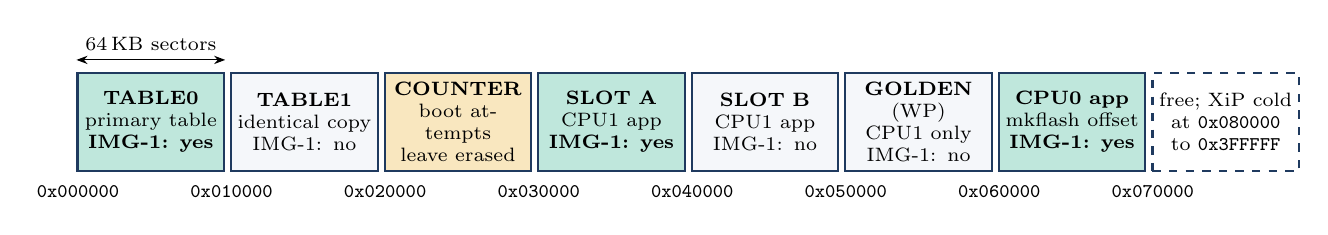
\begin{tikzpicture}[font=\scriptsize,
  sec/.style={draw=accent,thick,minimum height=1.25cm,align=center,inner sep=2pt,text width=1.72cm},
  >={Stealth[length=4pt]}]
\def\w{1.95}
\node[sec,fill=gQspi!25] (s0) at (0*\w,0) {\textbf{TABLE0}\\ primary table\\ \textbf{IMG-1: yes}};
\node[sec,fill=rowgray] (s1) at (1*\w,0) {\textbf{TABLE1}\\ identical copy\\ IMG-1: no};
\node[sec,fill=gRmii!25] (s2) at (2*\w,0) {\textbf{COUNTER}\\ boot attempts\\ leave erased};
\node[sec,fill=gQspi!25] (s3) at (3*\w,0) {\textbf{SLOT A}\\ CPU1 app\\ \textbf{IMG-1: yes}};
\node[sec,fill=rowgray] (s4) at (4*\w,0) {\textbf{SLOT B}\\ CPU1 app\\ IMG-1: no};
\node[sec,fill=rowgray] (s5) at (5*\w,0) {\textbf{GOLDEN} (WP)\\ CPU1 only\\ IMG-1: no};
\node[sec,fill=gQspi!25] (s6) at (6*\w,0) {\textbf{CPU0 app}\\ mkflash offset\\ \textbf{IMG-1: yes}};
\node[sec,fill=white,dashed] (s7) at (7*\w,0) {free; XiP cold\\ at \texttt{0x080000}\\ to \texttt{0x3FFFFF}};
\foreach \i/\a in {0/0x000000,1/0x010000,2/0x020000,3/0x030000,4/0x040000,5/0x050000,6/0x060000,7/0x070000}{
  \node[anchor=north,font=\scriptsize\ttfamily] at ($(s\i.south west)+(0.02,-0.05)$) {\a};}
\draw[<->] ($(s0.north west)+(0,0.15)$) -- node[above,font=\scriptsize] {64\,KB sectors} ($(s0.north east)+(0,0.15)$);
\end{tikzpicture}
\caption[QSPI flash layout]{QSPI flash layout (offsets within the flash; XiP base \texttt{0x24000000}). Green: sectors that IMG-1 (TABLE0-only) writes. Sources: \src{AMAP:376-381}; \src{MKF:120-143}.}
\label{fig:flash}
\end{figure}

\textbf{Table format (v2, little-endian).} The 32-byte header holds magic \texttt{0x424F4F54} ("BOOT") at +0x00, version 2 at +0x04, \sig{num_entries} at +0x08, \sig{seq} at +0x0C, \sig{table_crc} at +0x10, \sig{active_note} at +0x14, and reserved words. Each 32-byte entry holds \sig{stage1_offset}, \sig{stage1_size}, \sig{app_offset}, \sig{app_size}, \sig{flags} (bit 0 valid), \sig{stage1_crc}, \sig{app_crc} and a reserved word. \sig{table_crc} is CRC32-IEEE (reflected, as \sig{binascii.crc32}) over table bytes [\texttt{0x14}, \texttt{0x20} + $n\times$\texttt{0x20}) \src{AMAP:393-438}.

\textbf{Boot-counter policy.} Each ROM boot programs one \texttt{0xFF}$\to$\texttt{0x00} byte. A count $\ge$ 2 demotes the primary table. Confirmation means CPU1 publishes the boot-confirm token and CPU0, which owns the flash, erases the counter sector \src{NMS/firmware/include/nanosoc_boot_confirm.h:8-26}. With TABLE0 only, the demoted primary is still tried last, so the image keeps booting.

\newpage
% =====================================================================
\section{Full pad list with bond-opening coordinates}\label{app:pads}
% =====================================================================
Generated from \src{CSV} by \sig{figures/gen_figs.py}. Coordinates are bond-\emph{opening} centres in \textmu m, origin lower-left. ``Design'' is the 1600 $\times$ 2000\,\textmu m frame; ``seal ring'' adds 20\,\textmu m, giving the 1640 $\times$ 2040\,\textmu m frame. Row: o = outer (\sig{PAD70GU_SL}), i = inner (\sig{PAD70NU_SL}). Openings are 58\,\textmu m along the edge by 66\,\textmu m deep. Order: left edge bottom to top, top edge left to right, right edge bottom to top, bottom edge left to right.

{\footnotesize
\setlength{\tabcolsep}{4pt}
\renewcommand{\arraystretch}{1.08}
\begin{longtable}{@{}rllllcrrrr@{}}
\toprule
\rowcolor{headgray}[0pt][0pt] & & & & & & \multicolumn{2}{c}{\hd{Design frame}} & \multicolumn{2}{c}{\hd{Seal-ring frame}}\\
\rowcolor{headgray}[0pt][0pt]\hd{\#} & \hd{Signal} & \hd{Instance (BuPAD\_/uPAD\_)} & \hd{Edge} & \hd{Row} & \hd{IO cell} & \hd{x} & \hd{y} & \hd{x} & \hd{y}\\
\midrule
\endfirsthead
\toprule
\rowcolor{headgray}[0pt][0pt]\hd{\#} & \hd{Signal} & \hd{Instance} & \hd{Edge} & \hd{Row} & \hd{IO cell} & \hd{x} & \hd{y} & \hd{x} & \hd{y}\\
\midrule
\endhead
\bottomrule
\multicolumn{10}{@{}l}{\scriptsize\textsuperscript{a} The CSV labels this bond pad \sig{edge=top}; it is on the right edge (IO cell row 95 and x = 1513\,\textmu m).}\\
\endlastfoot
1 & TL\_RX0 & \texttt{TL\_RX\_0} & left & o & \texttt{PDDW16DGZ\_G} & 36.8 & 162.5 & 56.8 & 182.5 \\
2 & TL\_RX1 & \texttt{TL\_RX\_1} & left & i & \texttt{PDDW16DGZ\_G} & 138.8 & 229.5 & 158.8 & 249.5 \\
3 & TL\_RX2 & \texttt{TL\_RX\_2} & left & o & \texttt{PDDW16DGZ\_G} & 36.8 & 296.5 & 56.8 & 316.5 \\
4 & TL\_RX3 & \texttt{TL\_RX\_3} & left & i & \texttt{PDDW16DGZ\_G} & 138.8 & 363.5 & 158.8 & 383.5 \\
5 & VDDIO & \texttt{VDDIO\_L\_0} & left & o & \texttt{PVDD2DGZ\_G} & 36.8 & 430.5 & 56.8 & 450.5 \\
6 & VSSIO & \texttt{VSSIO\_L\_0} & left & i & \texttt{PVSS2DGZ\_G} & 138.8 & 497.5 & 158.8 & 517.5 \\
7 & TL\_CLK\_RX & \texttt{TL\_CLK\_RX} & left & o & \texttt{PDDW16DGZ\_G} & 36.8 & 564.5 & 56.8 & 584.5 \\
8 & TL\_RX4 & \texttt{TL\_RX\_4} & left & i & \texttt{PDDW16DGZ\_G} & 138.8 & 631.5 & 158.8 & 651.5 \\
9 & TL\_RX5 & \texttt{TL\_RX\_5} & left & o & \texttt{PDDW16DGZ\_G} & 36.8 & 698.5 & 56.8 & 718.5 \\
10 & TL\_RX6 & \texttt{TL\_RX\_6} & left & i & \texttt{PDDW16DGZ\_G} & 138.8 & 765.5 & 158.8 & 785.5 \\
11 & TL\_RX7 & \texttt{TL\_RX\_7} & left & o & \texttt{PDDW16DGZ\_G} & 36.8 & 832.5 & 56.8 & 852.5 \\
12 & I2C\_SCL & \texttt{I2C\_SCL} & left & i & \texttt{PDUW16DGZ\_G} & 138.8 & 899.5 & 158.8 & 919.5 \\
13 & I2C\_SDA & \texttt{I2C\_SDA} & left & o & \texttt{PDUW16DGZ\_G} & 36.8 & 966.5 & 56.8 & 986.5 \\
14 & VDDIO & \texttt{VDDIO\_L\_1} & left & i & \texttt{PVDD2DGZ\_G} & 138.8 & 1033.5 & 158.8 & 1053.5 \\
15 & VSSIO & \texttt{VSSIO\_L\_1} & left & o & \texttt{PVSS2DGZ\_G} & 36.8 & 1100.5 & 56.8 & 1120.5 \\
16 & TL\_TX0 & \texttt{TL\_TX\_0} & left & i & \texttt{PDDW16DGZ\_G} & 138.8 & 1167.5 & 158.8 & 1187.5 \\
17 & TL\_TX1 & \texttt{TL\_TX\_1} & left & o & \texttt{PDDW16DGZ\_G} & 36.8 & 1234.5 & 56.8 & 1254.5 \\
18 & TL\_TX2 & \texttt{TL\_TX\_2} & left & i & \texttt{PDDW16DGZ\_G} & 138.8 & 1301.5 & 158.8 & 1321.5 \\
19 & TL\_TX3 & \texttt{TL\_TX\_3} & left & o & \texttt{PDDW16DGZ\_G} & 36.8 & 1368.5 & 56.8 & 1388.5 \\
20 & VDDIO & \texttt{VDDIO\_L\_2} & left & i & \texttt{PVDD2DGZ\_G} & 138.8 & 1435.5 & 158.8 & 1455.5 \\
21 & VSSIO & \texttt{VSSIO\_L\_2} & left & o & \texttt{PVSS2DGZ\_G} & 36.8 & 1502.5 & 56.8 & 1522.5 \\
22 & TL\_CLK\_TX & \texttt{TL\_CLK\_TX} & left & i & \texttt{PDDW16DGZ\_G} & 138.8 & 1569.5 & 158.8 & 1589.5 \\
23 & TL\_TX4 & \texttt{TL\_TX\_4} & left & o & \texttt{PDDW16DGZ\_G} & 36.8 & 1636.5 & 56.8 & 1656.5 \\
24 & TL\_TX5 & \texttt{TL\_TX\_5} & left & i & \texttt{PDDW16DGZ\_G} & 138.8 & 1703.5 & 158.8 & 1723.5 \\
25 & TL\_TX6 & \texttt{TL\_TX\_6} & left & o & \texttt{PDDW16DGZ\_G} & 36.8 & 1770.5 & 56.8 & 1790.5 \\
26 & TL\_TX7 & \texttt{TL\_TX\_7} & left & i & \texttt{PDDW16DGZ\_G} & 138.8 & 1837.5 & 158.8 & 1857.5 \\
27 & VDDIO (POC) & \texttt{VDDIO\_T\_0} & top & o & \texttt{PVDD2POC\_G} & 162.5 & 1963.2 & 182.5 & 1983.2 \\
28 & VDD & \texttt{VDD\_T\_0} & top & i & \texttt{PVDD1DGZ\_G} & 242.5 & 1861.2 & 262.5 & 1881.2 \\
29 & VSS & \texttt{VSS\_T\_0} & top & o & \texttt{PVSS1DGZ\_G} & 322.5 & 1963.2 & 342.5 & 1983.2 \\
30 & NRST & \texttt{NRST\_I} & top & i & \texttt{PDDW04DGZ\_G} & 402.5 & 1861.2 & 422.5 & 1881.2 \\
31 & SWDCK & \texttt{SWDCK\_I} & top & o & \texttt{PDDW04DGZ\_G} & 482.5 & 1963.2 & 502.5 & 1983.2 \\
32 & CLK & \texttt{CLK\_I} & top & i & \texttt{PDDW04DGZ\_G} & 562.5 & 1861.2 & 582.5 & 1881.2 \\
33 & TEST & \texttt{TEST\_I} & top & o & \texttt{PDDW04DGZ\_G} & 642.5 & 1963.2 & 662.5 & 1983.2 \\
34 & SE & \texttt{SE\_I} & top & i & \texttt{PDDW04DGZ\_G} & 722.5 & 1861.2 & 742.5 & 1881.2 \\
35 & VDD & \texttt{VDD\_T\_1} & top & o & \texttt{PVDD1DGZ\_G} & 802.5 & 1963.2 & 822.5 & 1983.2 \\
36 & SWDIO & \texttt{SWDIO\_IO} & top & i & \texttt{PDUW08DGZ\_G} & 882.5 & 1861.2 & 902.5 & 1881.2 \\
37 & VSS & \texttt{VSS\_T\_1} & top & o & \texttt{PVSS1DGZ\_G} & 962.5 & 1963.2 & 982.5 & 1983.2 \\
38 & VDDIO & \texttt{VDDIO\_T\_1} & top & i & \texttt{PVDD2DGZ\_G} & 1042.5 & 1861.2 & 1062.5 & 1881.2 \\
39 & VDDIO & \texttt{VDDIO\_T\_2} & top & o & \texttt{PVDD2DGZ\_G} & 1122.5 & 1963.2 & 1142.5 & 1983.2 \\
40 & VSSIO & \texttt{VSSIO\_T\_0} & top & i & \texttt{PVSS2DGZ\_G} & 1202.5 & 1861.2 & 1222.5 & 1881.2 \\
41 & VSSIO & \texttt{VSSIO\_T\_1} & top & o & \texttt{PVSS2DGZ\_G} & 1282.5 & 1963.2 & 1302.5 & 1983.2 \\
42 & VDD & \texttt{VDD\_T\_2} & top & i & \texttt{PVDD1DGZ\_G} & 1362.5 & 1861.2 & 1382.5 & 1881.2 \\
43 & VSSIO & \texttt{VSSIO\_T\_2} & top & o & \texttt{PVSS2DGZ\_G} & 1442.5 & 1963.2 & 1462.5 & 1983.2 \\
44 & VDDIO & \texttt{VDDIO\_R\_0} & right & o & \texttt{PVDD2DGZ\_G} & 1563.2 & 162.5 & 1583.2 & 182.5 \\
45 & VSSIO & \texttt{VSSIO\_R\_0} & right & i & \texttt{PVSS2DGZ\_G} & 1461.2 & 242.5 & 1481.2 & 262.5 \\
46 & RMII\_MDC & \texttt{RMII\_MDC} & right & o & \texttt{PDDW16DGZ\_G} & 1563.2 & 322.5 & 1583.2 & 342.5 \\
47 & RMII\_REF\_CLK & \texttt{RMII\_REF\_CLK} & right & i & \texttt{PDDW04DGZ\_G} & 1461.2 & 402.5 & 1481.2 & 422.5 \\
48 & RMII\_RXD0 & \texttt{RMII\_RXD0} & right & o & \texttt{PDDW04DGZ\_G} & 1563.2 & 482.5 & 1583.2 & 502.5 \\
49 & VDDIO & \texttt{VDDIO\_R\_1} & right & i & \texttt{PVDD2DGZ\_G} & 1461.2 & 562.5 & 1481.2 & 582.5 \\
50 & VSSIO & \texttt{VSSIO\_R\_1} & right & o & \texttt{PVSS2DGZ\_G} & 1563.2 & 642.5 & 1583.2 & 662.5 \\
51 & RMII\_RXD1 & \texttt{RMII\_RXD1} & right & i & \texttt{PDDW04DGZ\_G} & 1461.2 & 722.5 & 1481.2 & 742.5 \\
52 & RMII\_TXD0 & \texttt{RMII\_TXD0} & right & o & \texttt{PDDW16DGZ\_G} & 1563.2 & 802.5 & 1583.2 & 822.5 \\
53 & RMII\_TXD1 & \texttt{RMII\_TXD1} & right & i & \texttt{PDDW16DGZ\_G} & 1461.2 & 882.5 & 1481.2 & 902.5 \\
54 & RMII\_TX\_EN & \texttt{RMII\_TX\_EN} & right & o & \texttt{PDDW16DGZ\_G} & 1563.2 & 962.5 & 1583.2 & 982.5 \\
55 & RMII\_MDIO & \texttt{RMII\_MDIO} & right & i & \texttt{PDDW16DGZ\_G} & 1461.2 & 1042.5 & 1481.2 & 1062.5 \\
56 & RMII\_CRS\_DV & \texttt{RMII\_CRS\_DV} & right & o & \texttt{PDDW04DGZ\_G} & 1563.2 & 1122.5 & 1583.2 & 1142.5 \\
57 & VDDIO & \texttt{VDDIO\_R\_2} & right & i & \texttt{PVDD2DGZ\_G} & 1461.2 & 1202.5 & 1481.2 & 1222.5 \\
58 & VSSIO & \texttt{VSSIO\_R\_2} & right & o & \texttt{PVSS2DGZ\_G} & 1563.2 & 1282.5 & 1583.2 & 1302.5 \\
59 & HOSTIO0 & \texttt{HOST\_IO\_0} & right & i & \texttt{PDDW16DGZ\_G} & 1461.2 & 1362.5 & 1481.2 & 1382.5 \\
60 & HOSTIO1 & \texttt{HOST\_IO\_1} & right & o & \texttt{PDDW16DGZ\_G} & 1563.2 & 1442.5 & 1583.2 & 1462.5 \\
61 & HOSTIO2 & \texttt{HOST\_IO\_2} & right & i & \texttt{PDDW16DGZ\_G} & 1461.2 & 1522.5 & 1481.2 & 1542.5 \\
62 & HOSTIO3 & \texttt{HOST\_IO\_3} & right & o & \texttt{PDDW16DGZ\_G} & 1563.2 & 1602.5 & 1583.2 & 1622.5 \\
63 & HOSTIO4 & \texttt{HOST\_IO\_4} & right & i & \texttt{PDDW16DGZ\_G} & 1461.2 & 1682.5 & 1481.2 & 1702.5 \\
64 & HOSTIO5 & \texttt{HOST\_IO\_5} & right & o & \texttt{PDDW16DGZ\_G} & 1563.2 & 1762.5 & 1583.2 & 1782.5 \\
65 & HOSTIO6\textsuperscript{a} & \texttt{HOST\_IO\_6} & right & i & \texttt{PDDW16DGZ\_G} & 1461.2 & 1842.5 & 1481.2 & 1862.5 \\
66 & VDDIO & \texttt{VDDIO\_B\_0} & bottom & o & \texttt{PVDD2DGZ\_G} & 162.5 & 36.8 & 182.5 & 56.8 \\
67 & VSSIO & \texttt{VSSIO\_B\_0} & bottom & i & \texttt{PVSS2DGZ\_G} & 242.5 & 138.8 & 262.5 & 158.8 \\
68 & VDD & \texttt{VDD\_B\_1} & bottom & o & \texttt{PVDD1DGZ\_G} & 322.5 & 36.8 & 342.5 & 56.8 \\
69 & VSS & \texttt{VSS\_B\_0} & bottom & i & \texttt{PVSS1DGZ\_G} & 402.5 & 138.8 & 422.5 & 158.8 \\
70 & QSPI\_IO0 & \texttt{QSPI\_IO\_0} & bottom & o & \texttt{PDDW16DGZ\_G} & 482.5 & 36.8 & 502.5 & 56.8 \\
71 & QSPI\_IO1 & \texttt{QSPI\_IO\_1} & bottom & i & \texttt{PDDW16DGZ\_G} & 562.5 & 138.8 & 582.5 & 158.8 \\
72 & QSPI\_IO2 & \texttt{QSPI\_IO\_2} & bottom & o & \texttt{PDDW16DGZ\_G} & 642.5 & 36.8 & 662.5 & 56.8 \\
73 & VDDIO & \texttt{VDDIO\_B\_1} & bottom & i & \texttt{PVDD2DGZ\_G} & 722.5 & 138.8 & 742.5 & 158.8 \\
74 & VSSIO & \texttt{VSSIO\_B\_1} & bottom & o & \texttt{PVSS2DGZ\_G} & 802.5 & 36.8 & 822.5 & 56.8 \\
75 & QSPI\_IO3 & \texttt{QSPI\_IO\_3} & bottom & i & \texttt{PDDW16DGZ\_G} & 882.5 & 138.8 & 902.5 & 158.8 \\
76 & QSPI\_SCLK & \texttt{QSPI\_SCLK} & bottom & o & \texttt{PDDW16DGZ\_G} & 962.5 & 36.8 & 982.5 & 56.8 \\
77 & QSPI\_nCS & \texttt{QSPI\_nCS} & bottom & i & \texttt{PDDW16DGZ\_G} & 1042.5 & 138.8 & 1062.5 & 158.8 \\
78 & VDD & \texttt{VDD\_B\_0} & bottom & o & \texttt{PVDD1DGZ\_G} & 1122.5 & 36.8 & 1142.5 & 56.8 \\
79 & VSSIO & \texttt{VSSIO\_B\_2} & bottom & i & \texttt{PVSS2DGZ\_G} & 1202.5 & 138.8 & 1222.5 & 158.8 \\
80 & VDD & \texttt{VDD\_B\_2} & bottom & o & \texttt{PVDD1DGZ\_G} & 1282.5 & 36.8 & 1302.5 & 56.8 \\
81 & VSS & \texttt{VSS\_B\_1} & bottom & i & \texttt{PVSS1DGZ\_G} & 1362.5 & 138.8 & 1382.5 & 158.8 \\
82 & VDDIO & \texttt{VDDIO\_B\_2} & bottom & o & \texttt{PVDD2DGZ\_G} & 1442.5 & 36.8 & 1462.5 & 56.8 \\

\end{longtable}\addtocounter{table}{-1}}

% =====================================================================
\section{Address blocklist}\label{app:blocklist}
% =====================================================================
The host tools must enforce this list. HZ numbers are PROC's hazard IDs.

{\footnotesize
\setlength{\tabcolsep}{4pt}
\begin{longtable}{@{}P{0.45cm}P{3.6cm}P{3.0cm}P{6.2cm}P{2.3cm}@{}}
\toprule
\rowcolor{headgray}[0pt][0pt]\hd{\#} & \hd{Address / range} & \hd{Rule} & \hd{Why} & \hd{Source}\\
\midrule
\endhead
1 & \texttt{0x24000000--0x24FFFFFF} (QSPI XiP) & Never access from HOSTIO or SWD & HZ-6. With no flash the wrapper stalls for 65536/$f$; with flash, a CPU executing from XiP can livelock and the watchdog never fires & \src{PROC:1138}; \src{REG:204} \\
2 & \texttt{0x2E0321A0--0x2E0321B8} (whole band) & Never access & HZ-1. Uninterruptible AXI hang; power cycle to recover. \texttt{0x2E0321AC/B0/B4} also hard-stall the CPU & \src{PROC:1139}; \src{REG:160} \\
3 & \texttt{0x2F000000--0x2FFFFFFF} (peer aperture) & Never access: there is no peer die & HZ-2. No default responder. A failed read parks the port and the next access wedges the host & \src{PROC:1140} \\
4 & \texttt{0x2E032080} ROLE\_CFG & Never write, except in P2b with the B-1 loopback fitted & Starts TideLink TX clock and data toggling at the CLK rate; RX never calibrates without the loopback & \src{REG:78-98} \\
5 & \texttt{0x2E032020}, \texttt{024}, \texttt{038}, \texttt{15C}, \texttt{160}, \texttt{168} & Never read & HZ-8. Read-to-clear and auto-increment: a read is a write & \src{PROC:1142} \\
6 & \texttt{0x2C100000}, \texttt{0x2C100100}, \texttt{0x2C100200} & Never read in a sweep. Use the DBG page \texttt{0x2C100200} only on purpose & HZ-7. A read acquires the lock, and both cores are live & \src{PROC:591,1141} \\
7 & \texttt{0x2E000000--0x2E003FFF} & No writes & HZ-3 (while the link is up). Keep the habit on this board & \src{PROC:1115} \\
8 & \texttt{0x29000000} bit 1 & Never set & Inert but write-1-set and permanent & \src{PROC:1144} \\
9 & \texttt{0x29000000} bit 0 & Only in P10, on purpose & HZ-4. Irreversible until power-on & \src{PROC:719} \\
10 & \texttt{0x2A000020} = 2 (CPU1\_SWRST) & Expect the link to drop & HZ-5. Resets the whole fabric including HOSTIO & \src{PROC:848} \\
11 & Flash erase or program via \texttt{0x21000000} & Not on the first die & The only HOSTIO route to CPU0 firmware; a state the ROM cannot parse loses the boot & \src{PROC:1143} \\
12 & Apps \sig{default_slave_error_walk}, \sig{busfault_irq_route} & Never run & They poke \texttt{0x2E}/\texttt{0x2F} believing them unmapped & \src{REG:159-161} \\
13 & HIO-203/204/208 (Tier 2) & Never before firmware-dependent tests in the same power cycle & They wipe eth IMEM and shared SRAM & \src{PROC:1147} \\
14 & Two-master rule & Never two of \{DMA-250, DAP, ADP\} on CPU1's or the eth subsystem's memories at once & HSEL defect in rc4 & research report 01 \S7 \\
15 & DMA-250 with any address in \texttt{0x2E000000--0x2FFFFFFF} & Never (source or destination) & Erratum D2D-DMA: silent corruption, DONE with no error & \src{docs/chip-reference-manual/review/closure/item11-tl053.md} \\
\bottomrule
\end{longtable}\addtocounter{table}{-1}}

% =====================================================================
\section{Source references}\label{app:refs}
% =====================================================================
Repository paths are relative to the \sig{nanosoc-ethernet-chiplet} root, as read at \sig{914c9e4}.

{\footnotesize
\setlength{\tabcolsep}{4pt}
\begin{longtable}{@{}P{2.4cm}P{9.7cm}P{4.2cm}@{}}
\toprule
\rowcolor{headgray}[0pt][0pt]\hd{Alias} & \hd{Path} & \hd{Note}\\
\midrule
\endhead
REG & \src{docs/tapeout/67-rc4-issue-register.md} & rc4 issue register, 2026-09-23; newest authority. \textbf{Untracked} at \sig{914c9e4} \\
PROC & \src{docs/bringup/ASIC_FIRST_SILICON_HOSTIO_PROCEDURE.md} & HOSTIO first-silicon procedure; \S0.3 superseded by REG \\
PLAN & \src{docs/bringup/HOSTIO4_FUNCTIONAL_TEST_PLAN.md} & HOSTIO functional test plan (memory map) \\
BSC & \src{docs/bscan/BRINGUP.md} & Boundary-scan bring-up \\
PADS & \src{ASIC/tech_wrappers/tsmc65/nanosoc_eth_chiplet_pads.v} & Pad ring source; the rc4 netlist agrees \\
PNR & \src{ASIC/eth-chiplet/build/rc4-20260829/outputs/nanosoc_eth_chiplet_pads_rc4_pnr.v} & Shipping netlist \\
FP & \src{ASIC/eth-chiplet/build/rc4-20260829/db_rc4/nanosoc_eth_chiplet_pads.fp.gz} & rc4 floorplan \\
CSV & \src{ASIC/submissions/padring_as_built_rzG_20260823/nanosoc_eth_chiplet_pads_as_built_pads_only.csv} & Matches the rc4 floorplan on 168/168 rows \\
PTAB & \src{src/rtl/bscan/pad_table.json} & Pad REN/OEN ties, TAP pins, IDCODE \\
SDC & \src{ASIC/eth-chiplet/build/holdeco-20260827/work/nanosoc_eth_chiplet_pads_routed_src/mmmc/modes/default_constraint_mode/default_constraint_mode.sdc} & The SDC rc4 was timed with \\
UPF & \src{ASIC/genus-innovus/inputs/nanosoc_eth_chiplet_pads.upf} & Supply ranges \\
CB & \src{sys_desc/chip_boundary/nanosoc_eth_chiplet.yaml} & Chip boundary \\
NMS & \src{nanosoc-multicore-system/} & Submodule at \sig{2adcd34} \\
AMAP & \src{NMS/firmware/include/nanosoc_multicore_addrmap.h} & Address map, flash format \\
ROM1 & \src{NMS/firmware/bootloader/stage0_bootrom_chip_core/main.c} & CPU1 boot ROM source \\
ROM0 & \src{NMS/firmware/bootloader/stage0_bootrom/main.c} & CPU0 boot ROM source \\
flash\_pack.py & \src{NMS/nanosoc_arch_tech/firmware/testcodes/bootloader/flash_pack.py} & The v2 packer \\
MKF & \src{ASIC/gls-netlist/flash/mkflash.sh} & Wrapper; \sig{check_flash.py} alongside \\
RIG & \src{scripts/rig/eth_chiplet/} & HOSTIO client, suite, hostio\_fw \\
HFW & \src{scripts/rig/eth_chiplet/hostio_fw/README.md} & hostio\_fw ABI and signatures (locally modified at \sig{914c9e4}) \\
PRMU & \src{NMS/nanosoc_arch_tech/rtl/slcorem0p_tech/src/verilog/slcorem0p_prmu.v} & Clock and reset \\
XDBG & \src{docs/design/CROSS_DIE_DEBUG_PLAN.md} & DAP and APs \\
\bottomrule
\end{longtable}\addtocounter{table}{-1}}

\textbf{Research reports} (2026-09-30, inputs to this plan; they carry the full citation trail): 01 die and PCB electricals; 02 functionality, firmware and tests; 03 PCB tools, chip-on-board and parts; 04 die-card slot contract v0 (superseded); 05 flip-chip versus daughter card; 06 slot contract v1 (interchangeable die card / K26 FPGA card). Companion study: \sig{FPGA_DAUGHTER_CARD_OPTIONS.pdf} (this directory).

\textbf{External sources} (from report 03, checked 2026-09-30):
\begin{itemize}\raggedright
\item Würth Elektronik: wire-bonding design-rule poster v1.2, \url{https://www.we-online.com/files/pdf1/design-rules-wire-bonding-cbt-en.pdf}; webinar 108, \url{https://www.we-online.com/files/pdf1/presentation-webinar-108-wesystems-bonding-and-more-cbt-en.pdf}.
\item Europractice ASIC prototype packaging design rules 2024, \url{https://europractice-ic.com/wp-content/uploads/2020/06/ASIC_Prototype_Packaging_Design_Rules_2024.pdf}; packaging service, \url{https://europractice-ic.com/services/packaging/asic-packaging/}.
\item Zepler Cleanrooms back-end, \url{https://www.southampton.ac.uk/research/institutes-centres/zepler-cleanrooms/backend-dice-bond}.
\item PCBWay gold wire-bonding finish, \url{https://www.pcbway.com/capabilities.html}; JLCPCB ENEPIG vs ENIG, \url{https://jlcpcb.com/blog/enepig-vs-enig-surface-finishes}.
\item Samtec HSEC8 (\url{https://uk.rs-online.com/web/p/edge-connectors/1798778}); Samtec Q Strip; Eurocircuits HDI pool and gold-edge-connector option, \url{https://www.eurocircuits.com/services/hdi-pool/}; Technion TPT HB16 page (stage size, search snippet); arXiv 1112.1037 (Au stud bumps on single dies). AMD Kria K26 SOM data sheet DS987 v1.2 (tables 1, 22, 25), K24 data sheet DS985, K26 carrier design guide UG1091; Mouser UK stock and prices for SM-K26-XCL2GI and the K26C (2026-09-30); TI SN74CB3Q3245.
\item Parts: LAN8720A DS00002165B; TPS62869, TPS7A94, INA228 and TS3A27518E (ti.com); MX25R6435F (DigiKey); J-Link BASE (segger.com).
\item Tools: SKiDL \url{https://github.com/devbisme/skidl}; Diode \url{https://github.com/diodeinc/pcb}; KiCad CLI \url{https://docs.kicad.org/9.0/en/cli/cli.html}; Freerouting \url{https://github.com/freerouting/freerouting}; KiKit \url{https://github.com/yaqwsx/KiKit}.
\end{itemize}

\end{document}
